\documentclass[xcolor={usenames,dvipsnames}
    ,handout
]{beamer}

%
% ugly hack referring to the slides folder. Works for me.
%
\makeatletter
\def\input@path{{/Users/denilson/teaching/cmput391/git-slides/}}
\makeatother

% \usepackage[T1]{fontenc} % font encoding
% \usepackage{fontspec}
\usepackage{fontspec}


\makeatletter%
\@ifclassloaded{beamer}{%
  \usepackage{lmodern} %%% modern beamer style
  %%beamer style
  \usetheme{metropolis}
  \usefonttheme{professionalfonts}
  \setbeamercolor{background canvas}{bg=background}
  \setbeamercolor{frametitle}{bg=snow,fg=black}
  \setbeamercolor{title separator}{fg=snow}
  \setbeamercolor{alerted text}{fg=accent}

  \let\oldtitle\title
  \renewcommand{\title}[1]{\oldtitle{CMPUT391\\#1}}
  \author{Instructor: Denilson Barbosa}
  \date{\small University of Alberta}
  \institute{\today\vskip4em Slides by D. Barbosa, with suggested corrections and improvements by (in alphabetical order) C. Bins, D. Caminhas, K. Guhzva, Q. Lautischer, E. Macdonald, M. A. Nascimento, K. Newbury, M. Strobl, D. Sunderman, K. Wang, and K. Wong.}
  
  \titlegraphic{
\includegraphics[width=1.5cm]{../images/by-sa.png}~
  {\tiny This work is licensed under a Creative Commons Attribution 4.0 International License}}

  %%%% un-framed blocks
  \setbeamertemplate{blocks}[rounded][shadow=false]
}{}

\@ifpackageloaded{xcolor}{}{
  \usepackage{xcolor}
}
\makeatother

\setsansfont[BoldFont={Open Sans SemiBold}]{Open Sans}[Scale=0.9]
\setmonofont{Cousine}[Scale=0.875]
% \setmathtt{Cousine}[Scale=0.875]

%%%% highlighting text 
\usepackage{xspace}
\def\highlight#1{\colorbox{accent}{\textcolor{white}{#1}}\xspace}

\def\blue#1{\textcolor{blue}{#1}}

%
%
%
\usepackage{parskip}

\usepackage{subcaption} % needed for subfigures

\usepackage{wrapfig} % for figures "to the side of the text"

\usepackage{anyfontsize} % for egregious warnings

%
% Fonts
%
% \usepackage{amsmath}
% \usepackage{mathspec}
% \setmathtt[Scale=0.875]{Cousine}

%
% various packages for tables and colored tables
%
\usepackage{xcolor,colortbl}
\usepackage{tcolorbox}

\definecolor{accent}{RGB}{225,68,85}
\definecolor{highlight}{RGB}{170,68,153}
\definecolor{background}{rgb}{253,252,252}

\definecolor{sqlColor}{RGB}{119,119,17}

\definecolor{Cfunction}{RGB}{51,51,153}

\definecolor{stringColor}{RGB}{51,51,153}
\definecolor{datatypeColor}{RGB}{170,68,153}
\definecolor{functionColor}{RGB}{51,134,116}

\definecolor{exampleColor}{RGB}{51,34,136}
\definecolor{commentColor}{RGB}{112,68,225}

\definecolor{fern}{RGB}{80,118,66}

\definecolor{snow}{RGB}{240,240,230}
\definecolor{Gray}{gray}{0.85}

\definecolor{tupleBoxColor}{gray}{0.85}

\definecolor{Maroon}{RGB}{139,0,0}

%
% coloring of SQL code
%
\def\ColorSymbol#1{\textcolor{functionColor}{#1}}

%
% hihglight box
%
\usepackage{xspace}
\def\highlight#1{\colorbox{accent}{\textcolor{white}{#1}}\xspace}

%
% Tables
%
\usepackage{multirow}
\usepackage{multicol}

%
% CODE LISTINGS
%
\usepackage{listings}

%
% catch-all style meant to provide a clean and "empty" style
% from which all others build upon
%
\lstdefinestyle{cmput391}{
  style=,
  frame=no,
  tabsize=2,
  numbers=none,
  showstringspaces=false,
  numberstyle=\footnotesize,
  basicstyle=\ttfamily\footnotesize\color{black},
  numbersep=4pt,
  keywords=[1]{},
  keywords=[2]{},
  keywords=[3]{sh_lock,xl_lock,unlock,read,write,commit,abort},
  keywordstyle=[1]\ttfamily\bfseries\footnotesize,
  keywordstyle=[2]\ttfamily\footnotesize,
  keywordstyle=[3]\ttfamily\footnotesize\color{Maroon},
  emph=[1]{},
  emph=[2]{},
  emph=[3]{},
  emphstyle=[1]\ttfamily\footnotesize,
  emphstyle=[2]\ttfamily\footnotesize,
  emphstyle=[3]\ttfamily\footnotesize,
  commentstyle=\ttfamily\itshape\color{commentColor},
  stringstyle=\ttfamily\color{stringColor},
  moredelim=**[l][\itshape\color{commentColor}]{--},
  moredelim=**[is][\color{highlight}]{-|}{|-},
  moredelim=[is][\bfseries\color{highlight}]{-:}{:-},
  morestring=[s][\color{stringColor}]{"}{"},
  morecomment=[l]{--}
}

\lstdefinelanguage{DTD}{
  style=cmput391,
  morekeywords=[1]{DOCTYPE,ELEMENT,ATTLIST},
  keywordstyle=[1]\color{accent},
  literate = {\#PCDATA}{{\textcolor{Cfunction}{\#PCDATA}}}7
             {\#IMPLIED}{{\textcolor{Cfunction}{\#IMPLIED}}}8
}

\lstdefinelanguage{XPath}{
  style=cmput391,
  morekeywords={xs,integer,current,date,distinct,values,avg,text,id,count,position,and,or,not,boolean,number,sum,floor,ceiling,round,doc,eq,ne,gt,lt,ge,le},
  keywordstyle=\color{red},
  literate = {last(}{{\textcolor{functionColor}{last}(}}5 {@<}{{<}}1  
}

\lstdefinestyle{XQuery}{
  style=cmput391,
  keywords=[1]{if,then,else,and,or,some,every,satisfies,for,in,let,where,group,order,by,return,ascending},
  keywords=[2]{gt,lt,eq,ne,ge,le,not,or},
  keywords=[3]{text,sum,min,max,avg,len,position,number,boolean,floor,ceiling,round,%
               id,doc,count,current-date,distinct-values,xs:integer,subsequence},
  keywordstyle=[1]\bfseries\color{sqlColor},
  keywordstyle=[2]\color{accent},
  keywordstyle=[3]\color{functionColor},
  moredelim =[is][\color{blue}]{-:}{:-},
  moredelim =[s][\color{accent}]{<}{>},
  moredelim=**[s][\color{black}]{/}{\ },
  moredelim=*[s][\color{blue}]{\$}{\ },
  alsoletter=:{:,-},
  literate = {(}{{\textcolor{black}{(}}}{1} {)}{{\textcolor{black}{)}}}{1} 
             {\{}{{\textcolor{black}{\{}}}{1} {\}}{{\textcolor{black}{\}}}}{1} 
             {last(}{{\textcolor{functionColor}{last}(}}5 {@<}{{<}}1
}


\lstdefinestyle{SQL}{
  style=cmput391,
  language=SQL,
  sensitive={True},
  deletekeywords={year,Cast,MIN,MAX},
  morekeywords={ABORT,AFTER,BEFORE,REFERENCES,REFERENCING,WITH,COMMITTED,UNCOMMITTED,REPEATABLE,SERIALIZABLE},
  keywords=[2]{AVG,MIN,MAX,COUNT,SUM,NEW,OLD,strftime,date,length,RAISE,rowid,substr},
  keywords=[3]{BIGINT,CHAR,DATE,DECIMAL,INT,FLOAT,TEXT},
  keywordstyle=[1]\ttfamily\bfseries\color{sqlColor},
  keywordstyle=[2]\ttfamily\bfseries\color{functionColor},
  keywordstyle=[3]\ttfamily\bfseries\color{datatypeColor},
  moredelim=**[is][\ttfamily\bfseries\color{functionColor}]{(@}{@)},
  morestring=[s][\color{stringColor}]{'}{'},
  moredelim=[is][\bfseries\color{highlight}]{-:}{:-}
}


%
% lstlisting for command line examples
%
\lstdefinestyle{commandLine}{
  basicstyle=cmput391,
  keywordstyle=[1]\ttfamily\bfseries\color{functionColor},
  keywordstyle=[2]\ttfamily\bfseries\color{datatypeColor},
  moredelim=**[is][\color{accent}\bf]{@}{@}
  keywords=[1]{%
    grep},
  keywords=[2]{%
    postings}
}

%
% lstlisting for C code
%
\lstdefinestyle{C}{
  language=C,
  tabsize=2,
  basicstyle=\ttfamily\footnotesize,
  stringstyle=\color{stringColor},
  keywords=[2]{sqlite3_prepare_v2,sqlite3_bind_int64,sqlite3_step,sqlite3_exec},
  keywordstyle=[1]\ttfamily\bfseries\color{datatypeColor},
  keywordstyle=[2]\ttfamily\bfseries\color{functionColor},
  commentstyle=\ttfamily\itshape\color{commentColor},
  moredelim=**[is][\color{Cfunction}\bf\ttfamily]{@}{@}
}


\lstdefinestyle{Python}{
  language=Python,
  tabsize=2,
  basicstyle=\ttfamily\footnotesize,
  stringstyle=\color{stringColor},
  morekeywords=[1]{self,yield,Class,true,false,None},
  keywords=[2]{satisfies,from,Iterator,EOF,concatenate,advance,join,rewind},
  deletekeywords=[1]{from},
  keywordstyle=[1]\ttfamily\bfseries\color{datatypeColor},
  keywordstyle=[2]\ttfamily\bfseries\color{functionColor},
  commentstyle=\ttfamily\itshape\color{commentColor},
  moredelim=**[is][\color{Cfunction}\bf\ttfamily]{@}{@}
}



%
% lstlisting style for RDF/SPARQL
%
\lstdefinestyle{SPARQL}{
  style=cmput391,
  sensitive={True},
  keywords=[1]{BASE,PREFIX,SELECT,WHERE,FILTER,MINUS,NOT,EXISTS},
  keywordstyle=[1]\ttfamily\bfseries\color{sqlColor},
  moredelim=*[s][\color{Cfunction}]{?}{\ },
  moredelim=*[s][\color{Cfunction}]{@}{\ },
  morestring=[s][\color{datatypeColor}]{"}{"},
  literate =* {|}{{|}}1 {//}{{//}}2 {< }{< }{2}
}

%
% coloring of markup code
%
\lstdefinestyle{markup}{
  style=cmput391,
  literate =* {=}{{\color{sqlColor}{=}}}1,
  moredelim =* [s][\color{accent}]{<}{>},
  moredelim =** [is][\color{accent}]{@}{@},
  moredelim =** [is][\color{blue}]{-:}{:-},
  morecomment=[s]{<!--}{-->}
}

\lstdefinestyle{RDF}{
  style=cmput391,
  keywords=[1]{BASE,PREFIX},
  keywordstyle=[1]\ttfamily\bfseries\color{functionColor},
  alsoletter=:{:,-,@},
  literate = {prefix}{{\bfseries\textcolor{functionColor}{prefix}}}6 
             {:}{{\textcolor{functionColor}{:}}}1 
             {@}{{\textcolor{functionColor}{@}}}1,
  moredelim =* [s][\color{accent}]{<}{>},
  moredelim =** [is][\color{functionColor}]{-:}{:-},
  morecomment=[s]{<!--}{-->}
}




















%
% Tikz stuff, for cummulative diagrams and algebra trees
%
\usepackage{tikz} %commutative diagrams
\usepackage{tikz-cd} %commutative diagrams
\usetikzlibrary{positioning}% To get more advances positioning options
\usetikzlibrary{arrows,shapes,automata}
\usetikzlibrary{calc} % for calculations and hard-coded coordinates
\usetikzlibrary{tikzmark, fit, shapes.misc}
\usetikzlibrary{decorations.pathreplacing}
\usetikzlibrary{backgrounds} % to draw underneath other elements
\usepackage{stackengine} % to overlay tikz pictures over other things

\usepackage{pgfplots}
\pgfplotsset{compat=1.17}

%
%
% PGF arrowtip that looks like an X
%
%
\pgfarrowsdeclare{X}{X}
{
  \arrowsize=0.25pt
  \advance\arrowsize by .5\pgflinewidth
  \pgfarrowsleftextend{-4\arrowsize-.5\pgflinewidth}
  \pgfarrowsrightextend{.5\pgflinewidth}
}
{
  \arrowsize=0.2pt
  \advance\arrowsize by .5\pgflinewidth
  \pgfsetdash{}{0pt} % do not dash
  \pgfsetroundjoin   % fix join
  \pgfsetroundcap    % fix cap
  \pgfpathmoveto{\pgfpointorigin}
  \pgfpathlineto{\pgfpoint{-5\arrowsize}{5\arrowsize}}
  \pgfusepathqstroke
  \pgfpathmoveto{\pgfpointorigin}
  \pgfpathlineto{\pgfpoint{5\arrowsize}{-5\arrowsize}}
  \pgfusepathqstroke
  \pgfpathmoveto{\pgfpointorigin}
  \pgfpathlineto{\pgfpoint{-5\arrowsize}{-5\arrowsize}}
  \pgfusepathqstroke
  \pgfpathmoveto{\pgfpointorigin}
  \pgfpathlineto{\pgfpoint{5\arrowsize}{5\arrowsize}}
  \pgfusepathqstroke
}


%
%%% for algorithms and pseudocode
%
\usepackage{algorithm}
% \usepackage{algpseudocode}
\usepackage[noend]{algpseudocode}
\renewcommand{\algorithmicrequire}{\textbf{Input:}}
\renewcommand{\algorithmicensure}{\textbf{Output:}}
\algnewcommand\algorithmicforeach{\textbf{for each}}
\algdef{S}[FOR]{ForEach}[1]{\algorithmicforeach\ #1\ \algorithmicdo}
% style for comments inside algorithms
\renewcommand{\algorithmiccomment}[1]{\hspace*{1em}\textcolor{commentColor}{\%~\textit{#1}}} 

%
% to create boxes with verbatim and code-like content
%
\usepackage{verbatimbox}

%
% to crop/trim boxes!
%
\usepackage{trimclip}

%
% colored and framed boxes
%
\newenvironment{BOX}[1]{\begin{tcolorbox}[colback=snow!25,colframe=snow!40!black,title=#1]\small}{\end{tcolorbox}}



%
% math and symbols
%
\usepackage{mathtools}
\DeclarePairedDelimiter{\ceil}{\lceil}{\rceil}
\DeclarePairedDelimiter{\floor}{\lfloor}{\rfloor}
\usepackage{amsbsy} 
\usepackage{amssymb}
\usepackage{ifsym} % needed to produce the common outerjoin symbols

%
% for nice-looking enumerations and inlined enumerations
%
\usepackage[shortlabels,inline]{enumitem}



%%% outer join symbols
\newcommand\TextbookOuterJoin{%
  \mathrel{\ooalign{\hss$\Join$\hss\cr%
  \kern0.5ex\raise1ex\hbox{\scalebox{0.7}{$\circ$}}}}}

\newcommand\RightOuterJoin{%
  \mathrel{%
  	\ooalign{%
  		$\Join$\cr\kern1.25ex\raise0.0975ex\hbox{\scalebox{0.25}[0.8275]{$\sqsubset$}}}
  	}
}

\newcommand\LeftOuterJoin{%
  \mathrel{%
  	\ooalign{%
  		$\Join$\cr\kern-0.0125ex\raise0.0975ex\hbox{\scalebox{0.25}[0.8275]{$\sqsupset$}}}%
	}
}

\newcommand\FullOuterJoin{%
  \mathrel{%
  	\ooalign{%
  		$\Join$\cr\kern-0.0125ex\raise0.0975ex\hbox{\scalebox{0.25}[0.8275]{$\sqsupset$}}}%
  		\kern-0.45ex\raise0.0975ex\hbox{\scalebox{0.25}[0.8275]{$\sqsubset$}}
	}
}






\title{High Performance Databases and ``NoSQL''}

\begin{document}

\frame{\maketitle}

%%%%%%%%%%%%%%%%%%%%%%%%%
\begin{frame}{What is meant by NoSQL?}

\begin{block}{Is SQL a bad thing?}
\begin{columns}[onlytextwidth]
\begin{column}{0.75\textwidth}
The ``NoSQL movement'' started as frontal opposition to relational database systems in general. 
\end{column}
\begin{column}{0.25\textwidth}
\begin{center}

\includegraphics[width=0.75\textwidth]{./figures/noSQL.pdf}
\end{center}
\end{column}
\end{columns}
\end{block}

Over time, adopters of the movement realized that abandoning all of the relational technologies meant giving up too much.

Today, NoSQL is often used to mean \alert{Not Only} SQL. In other words, their proponents advocate using systems that support (at least a subset of) SQL in addition to other access methods and languages.

\end{frame}

\begin{frame}{Outline}
\tableofcontents
\end{frame}

\section{High Performance Computing Architectures}
%!TEX root = lec08_nosql.tex

\begin{frame}{DBMS processes}


\vskip1em

\begin{columns}[onlytextwidth]
\begin{column}{0.35\textwidth}
\begin{minipage}{1.25\textwidth}
\raggedright
From the Operating System point of view, a DBMS is implemented by a large number of independent processes, each handling one functionality of the system, and all accessing the same data in memory.

\vskip0.5em

We now look at ways of coping when the number of processes or the volume of data (or both) becomes too high for a ``standard'' server architecture.
\end{minipage}
\end{column}
\begin{column}{0.55\textwidth}
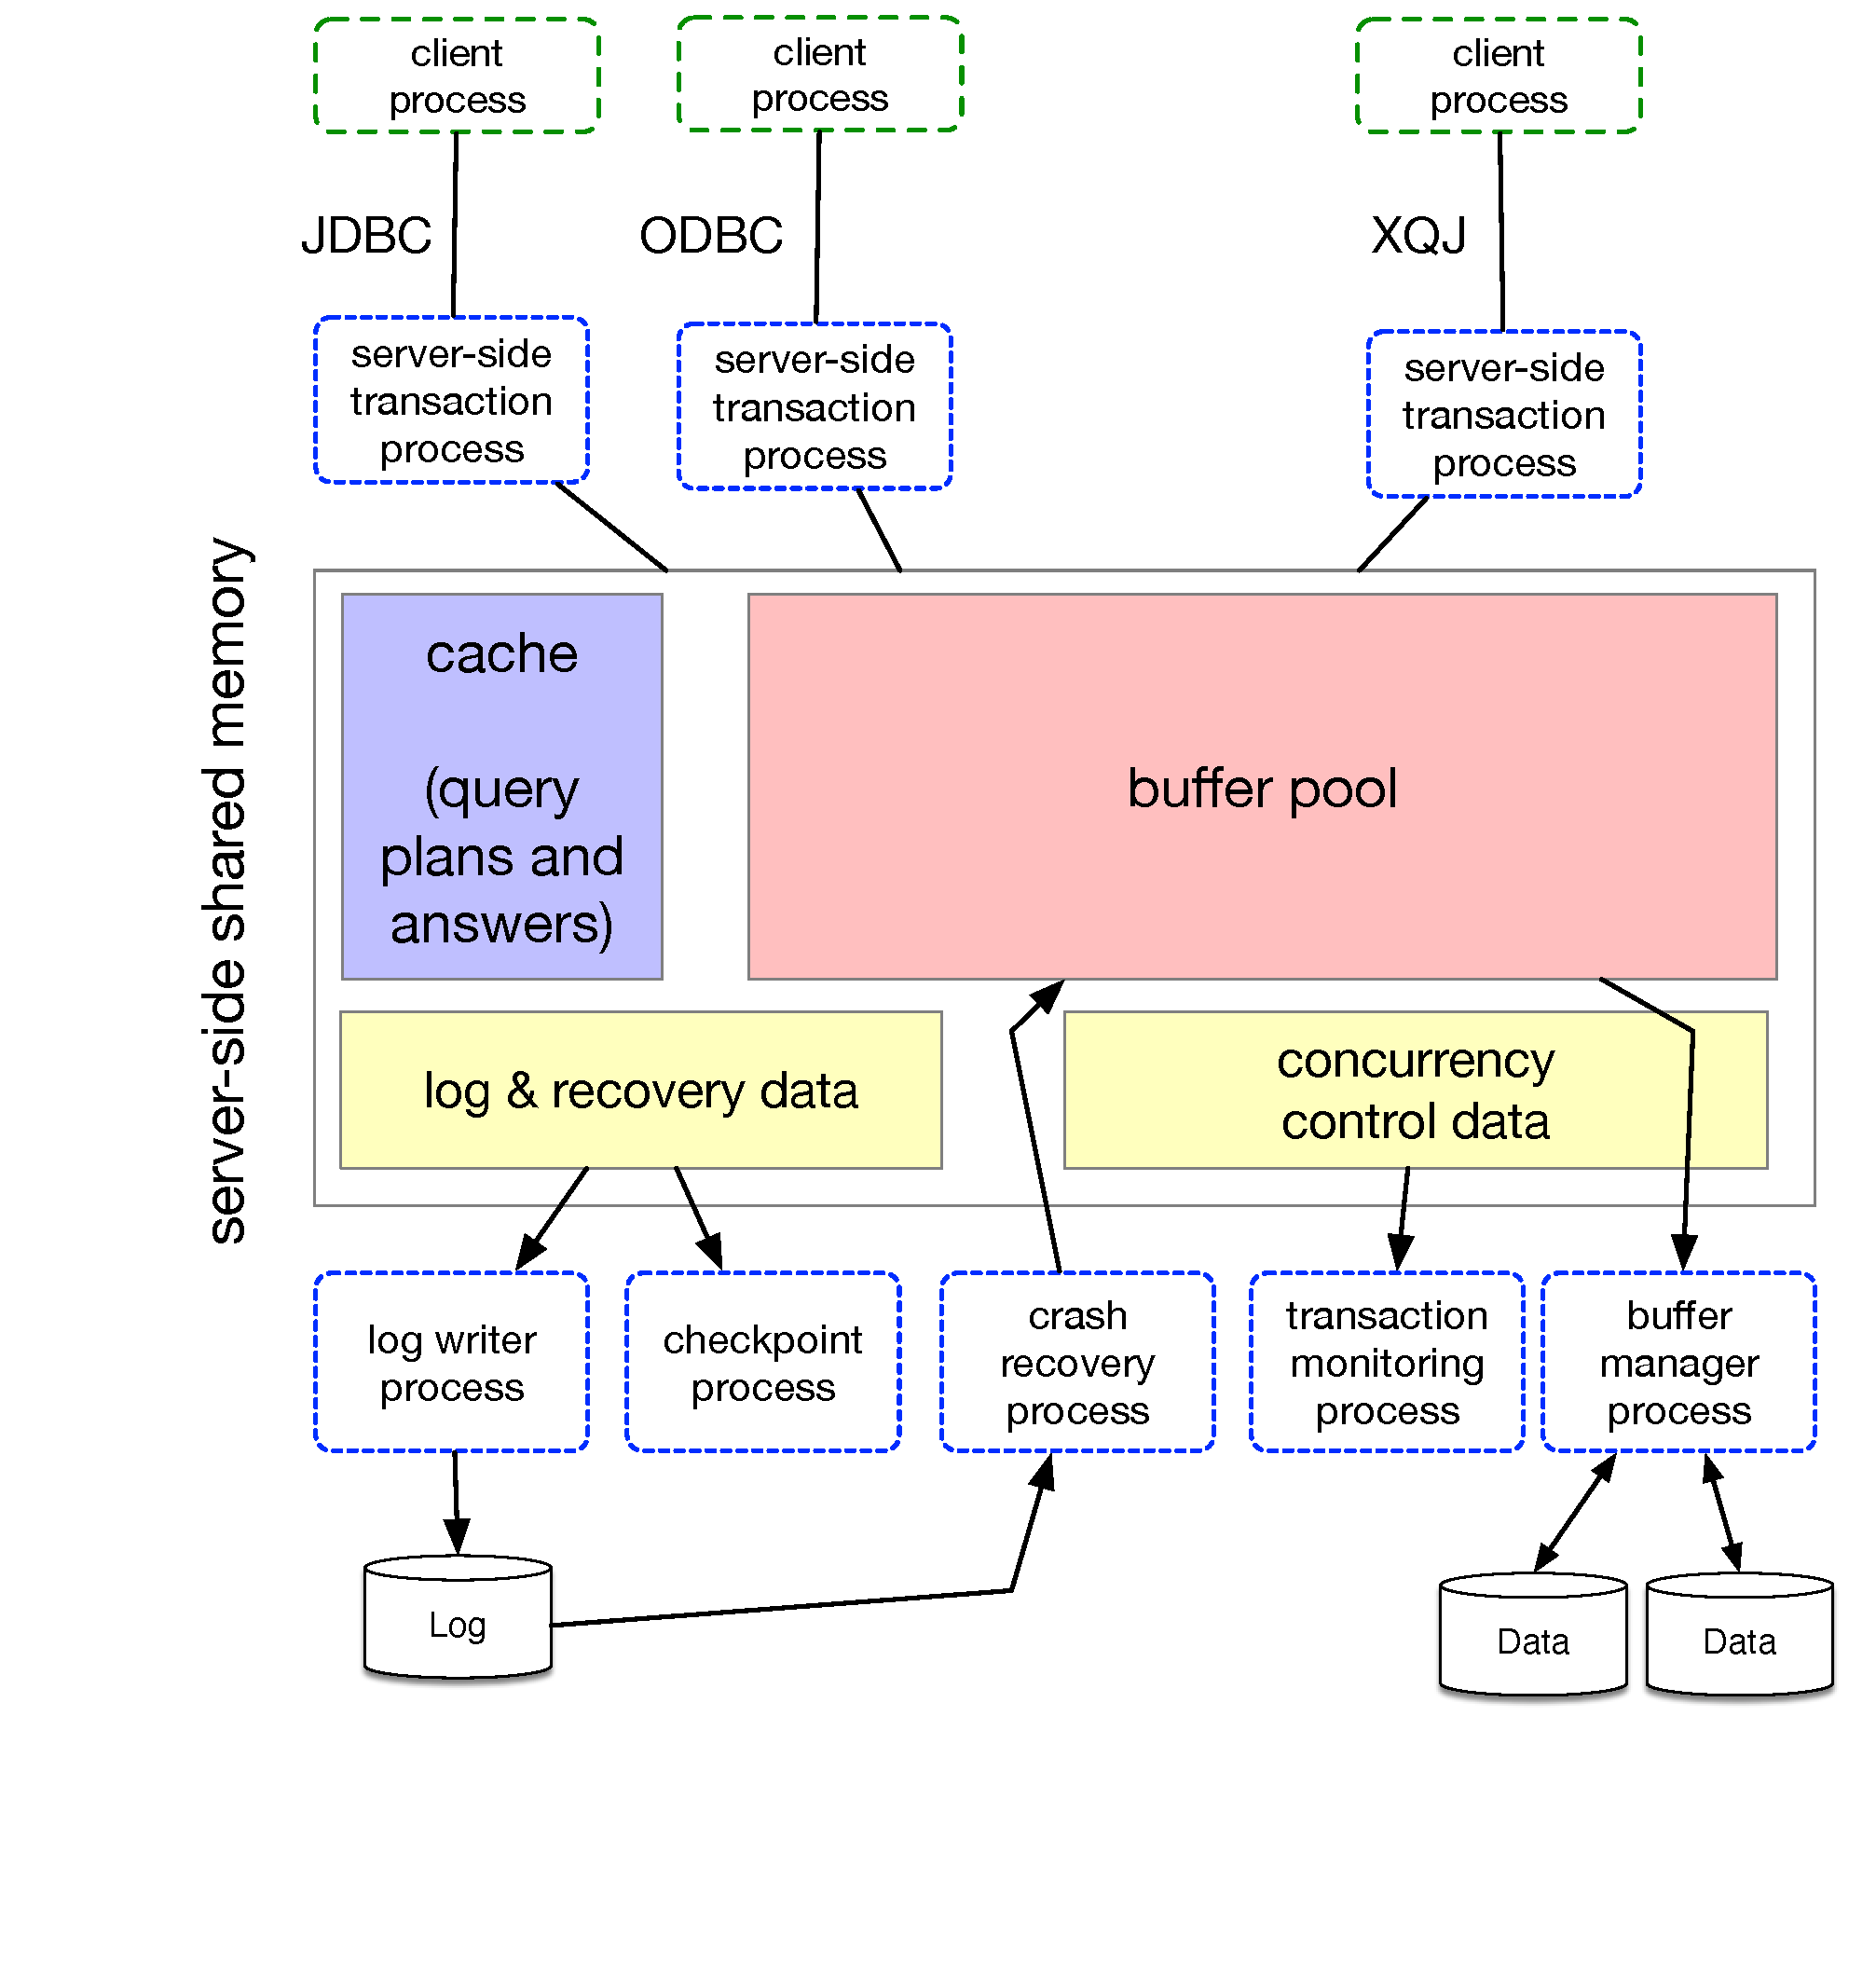
\includegraphics[width=1.1\textwidth]{figures/processes_memory_disks.eps}
\end{column}
\end{columns}
\end{frame}

\begin{frame}{Too much data?}

\begin{columns}[onlytextwidth]
\begin{column}{0.5\textwidth}
``Large'' databases nowadays are measured in \textbf{peta}bytes.

\vskip1em
Financial institutions and retailers are probably among the ones with the largest relational databases out there.
\end{column}
\begin{column}{0.4\textwidth}
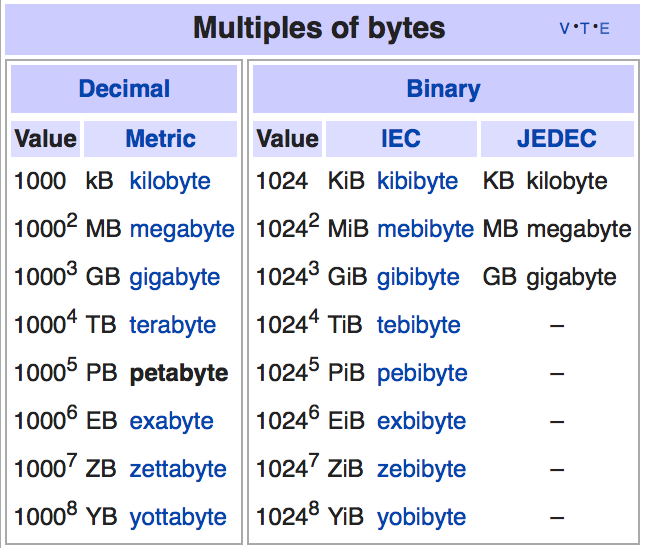
\includegraphics[width=1.1\textwidth]{figures/multiples_of_bytes.png}
\end{column}
\end{columns}

Some known very large databases:
\begin{itemize}[-,noitemsep,topsep=-10pt]
\item Facebook reported having a 30PB database in 2011
\item Google Maps was reported as 20PB in 2012
\item Google's crawl and associated metadata is reported at 10 exabytes
\item Scientific databases are often astronomical (in size too)
\end{itemize}
\end{frame}

\begin{frame}

\vskip3em

\begin{columns}[onlytextwidth]
\begin{column}{0.35\textwidth}
\begin{minipage}{1.25\textwidth}
\raggedright

With a large database, even the simplest queries become a challenge.

\vskip0.5em

Not too long ago, Google stored 25 billion pages. 

\vskip0.5em

At 20KB per page (ignoring figures, etc.), that would be 500 TB of raw data.
\end{minipage}
\end{column}
\begin{column}{0.45\textwidth}
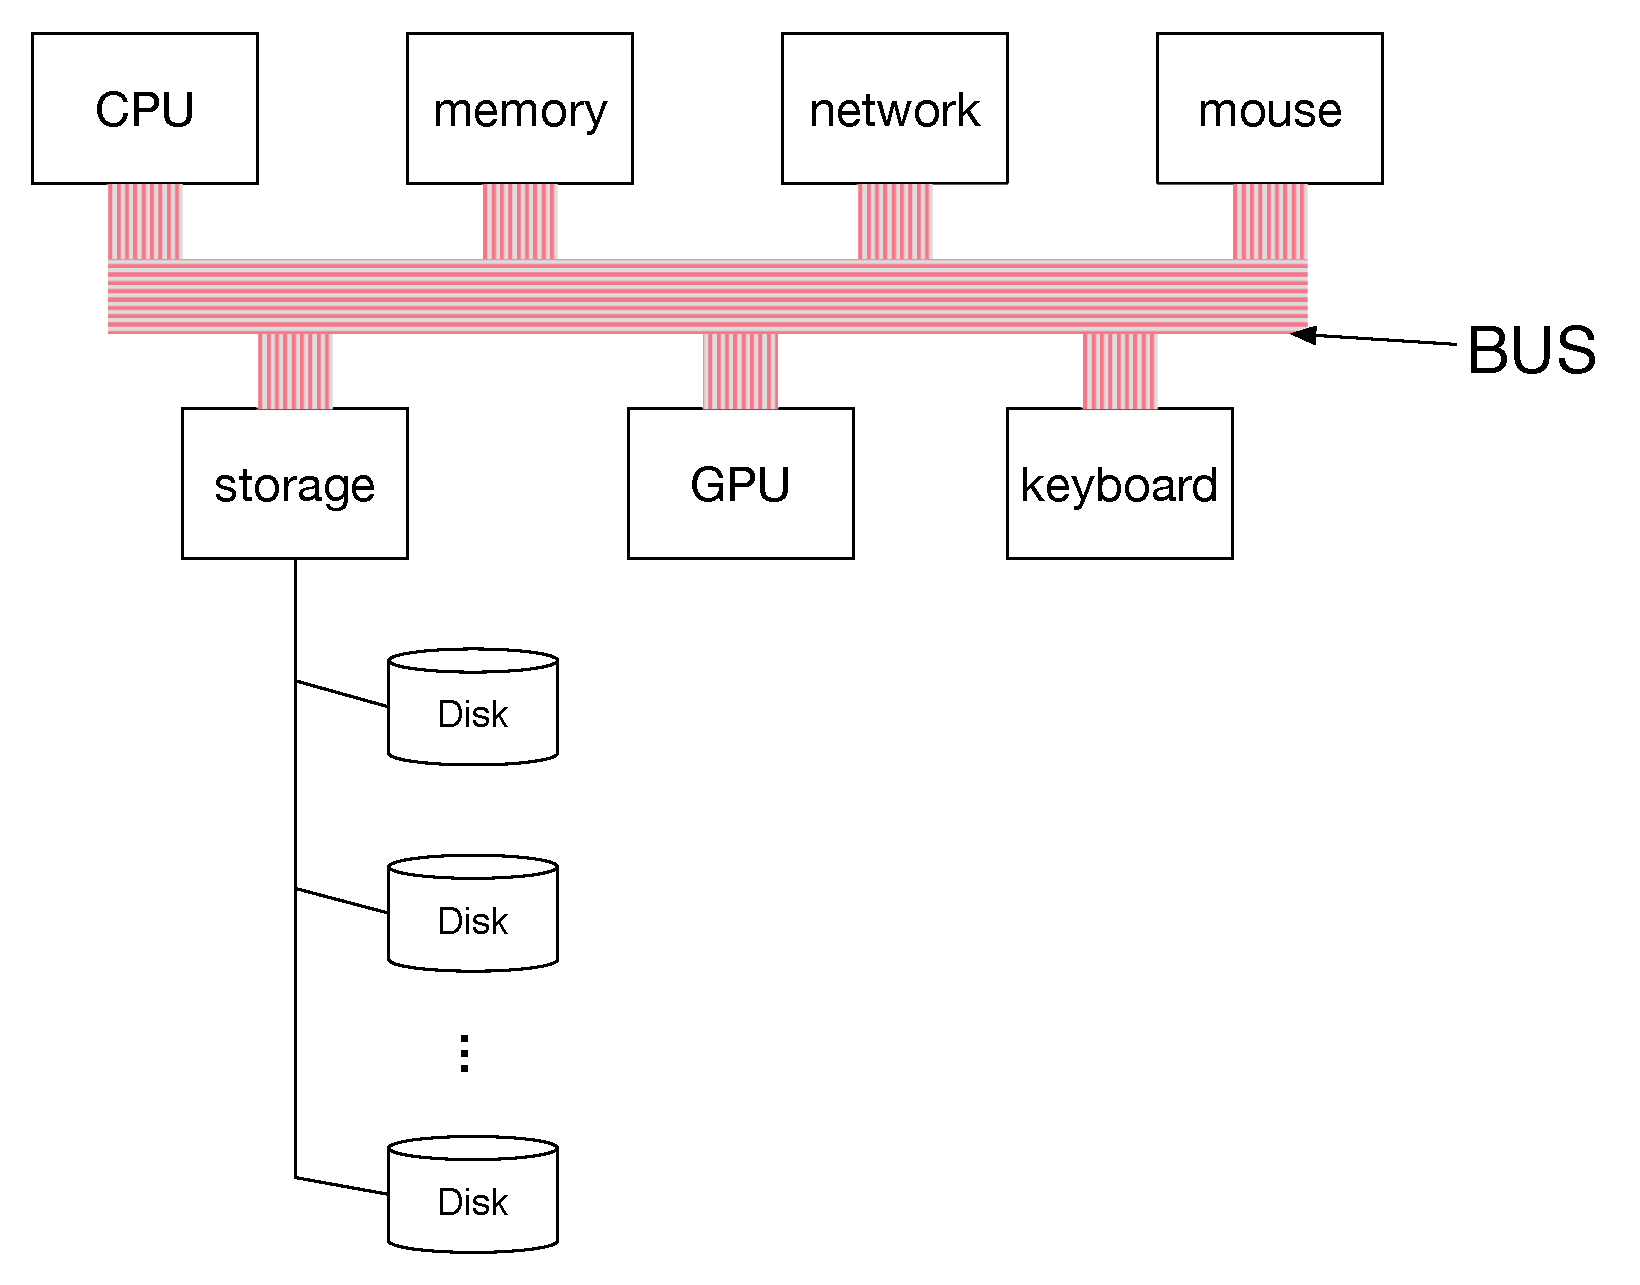
\includegraphics[width=1.1\textwidth]{../lec03_hardware/figures/von_neumann_architecture.eps}
\end{column}
\end{columns}

\vskip0.5em

How long would it take to run a query to find which web pages contain a link to \lstinline!ualberta.ca! on a ``standard server''?

With a fast 500MB/s BUS, \alert{the table scan would take at least}
\[\frac{500\cdot1024\cdot 1024 \text{ MB}}{500 \text{MB/s}}=1 M \text{seconds} \approx \text{ \alert{12 days}}\]
\end{frame}



\begin{frame}{Too many users?}

\begin{columns}[onlytextwidth]
\begin{column}{0.45\textwidth}
\begin{minipage}{1.25\textwidth}
\raggedright

Each connection to the database requires a ``server-side'' process which takes resources (memory for buffers).

\vskip0.5em

Also, each server-side process competes with the DBMS's own processes for CPU cycles.

\vskip0.5em

With a single CPU and 1,000 connected users, each requiring 1 second, it will take up to 15 minutes to serve them all.
\end{minipage}
\end{column}
\begin{column}{0.45\textwidth}
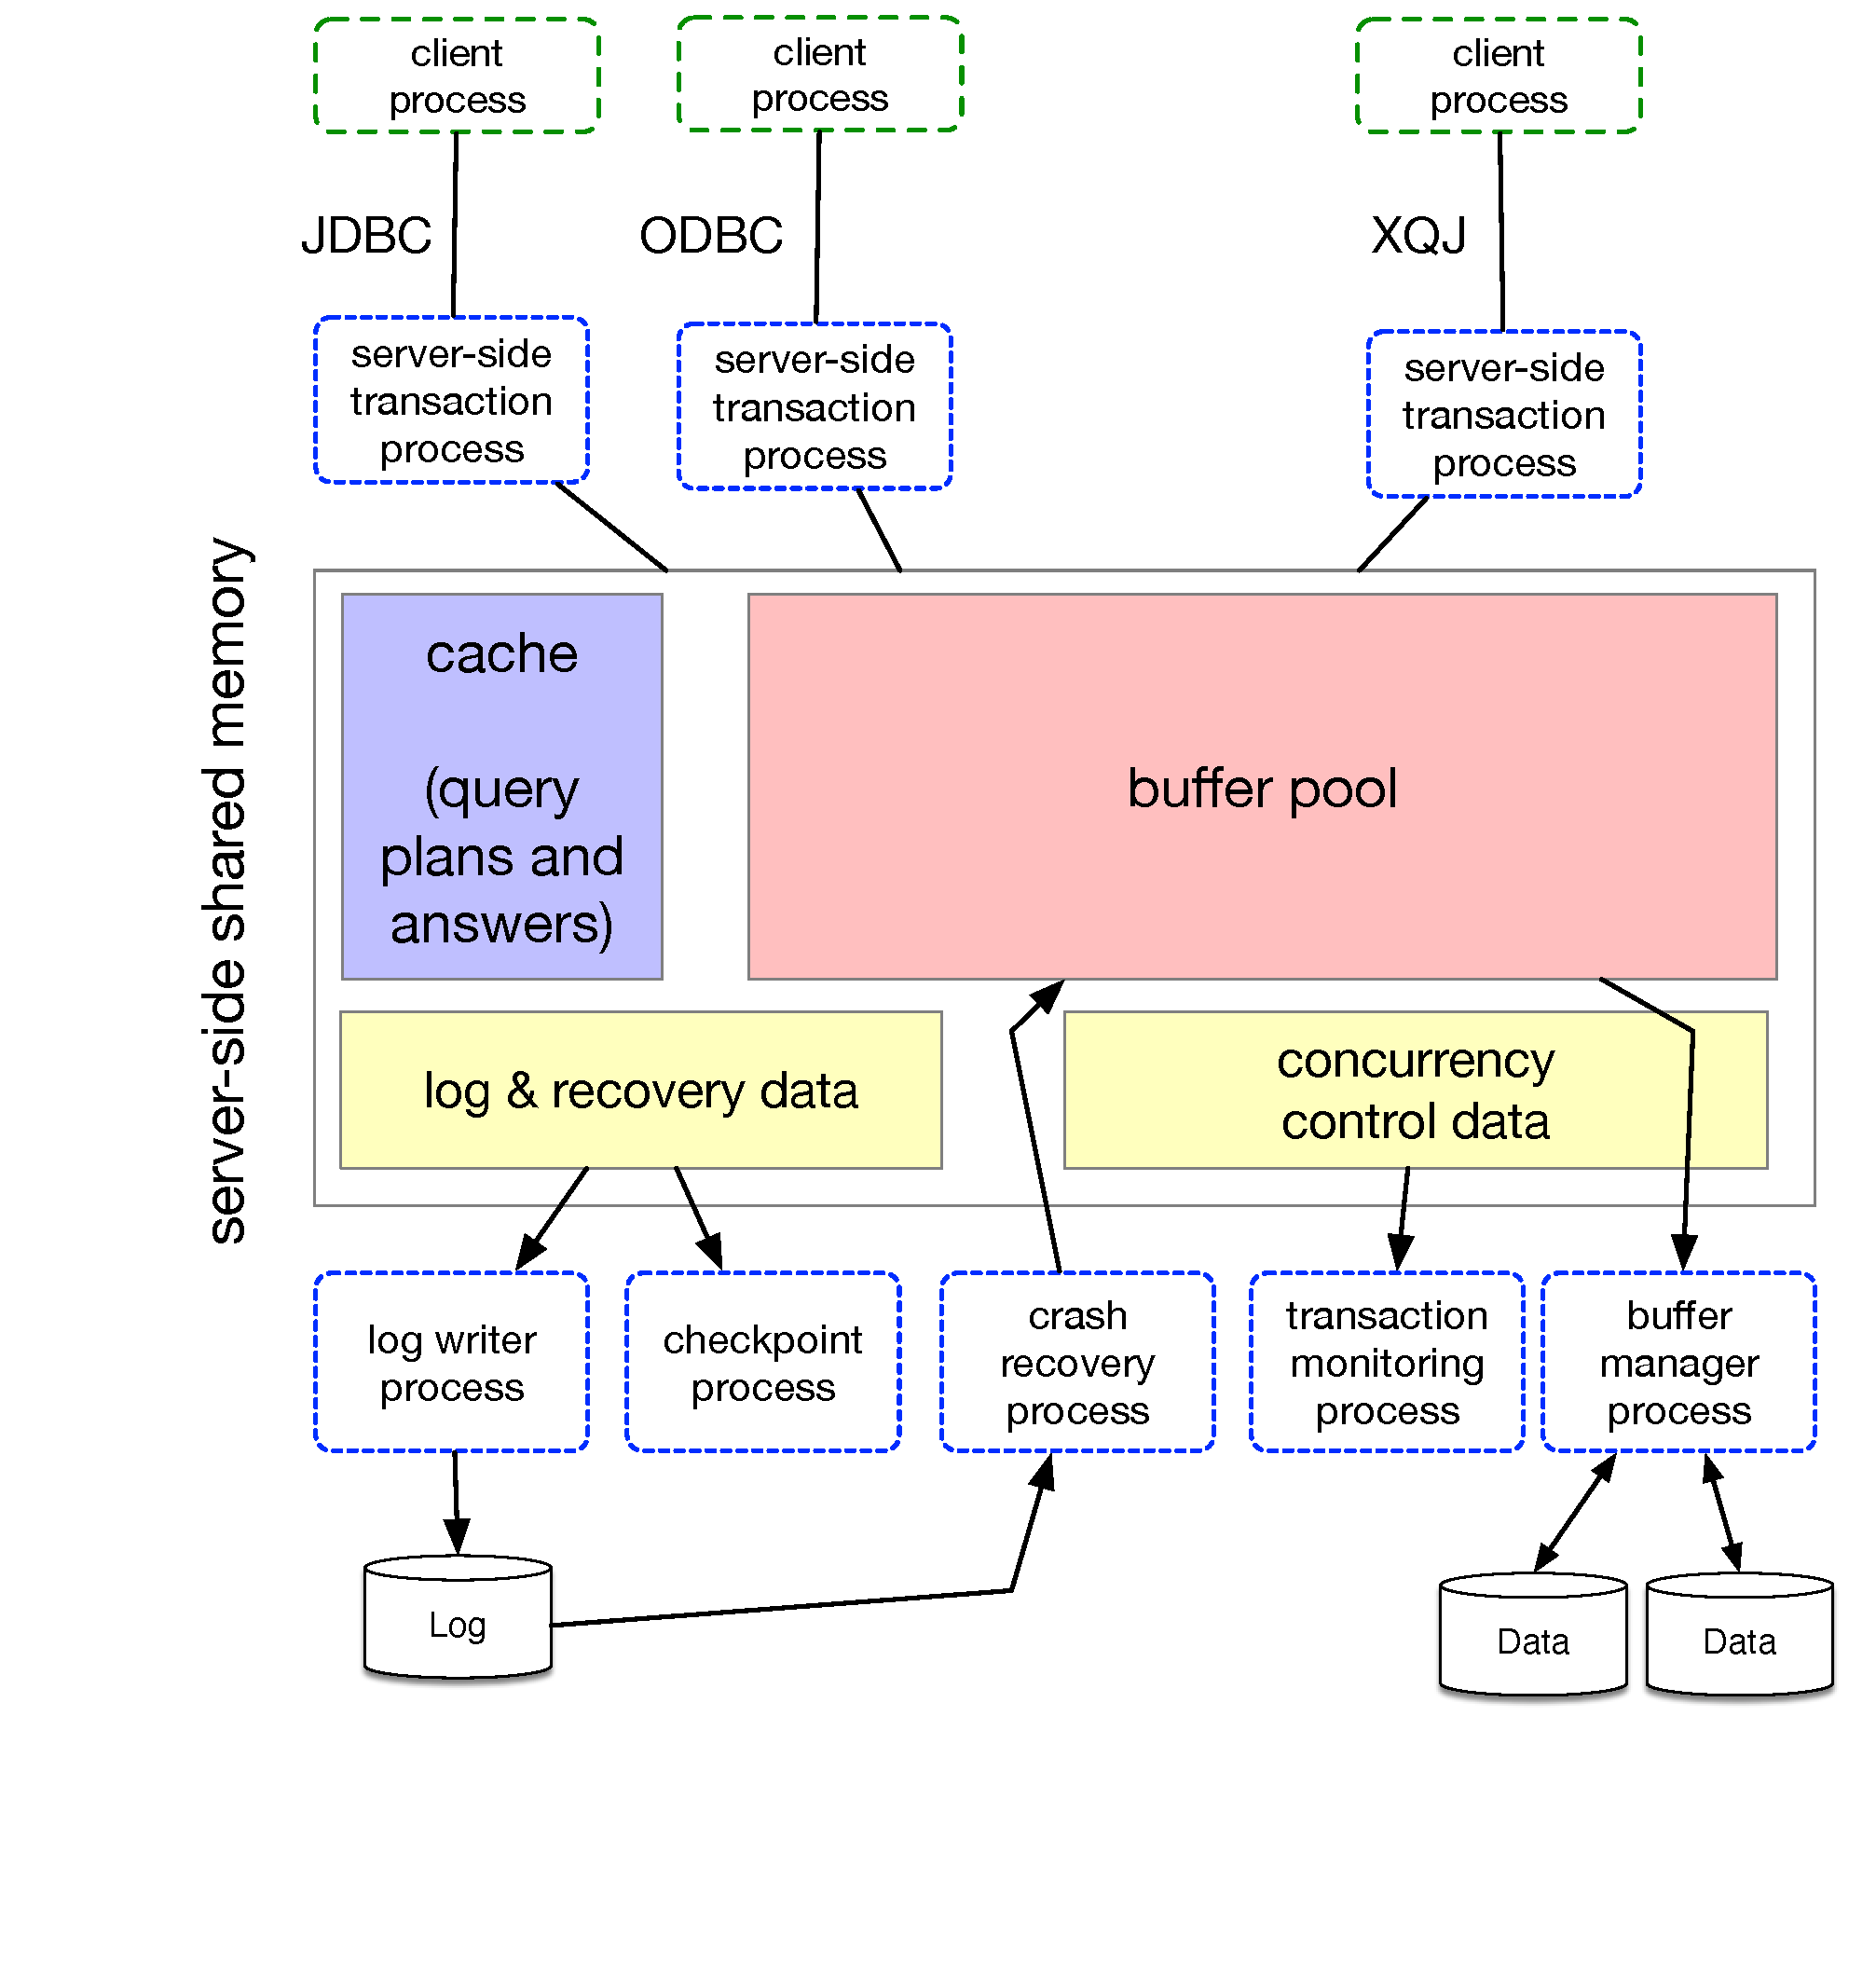
\includegraphics[width=1.1\textwidth]{figures/processes_memory_disks.eps}
\end{column}
\end{columns}
\end{frame}

\begin{frame}{Architectures for High Performance Computing}


\begin{columns}[onlytextwidth]
\begin{column}{0.45\textwidth}
The most modest step up from a standard Von Neumann architecture is to use a multi-core\footnotemark CPU:
\end{column}

\begin{column}{0.5\textwidth}
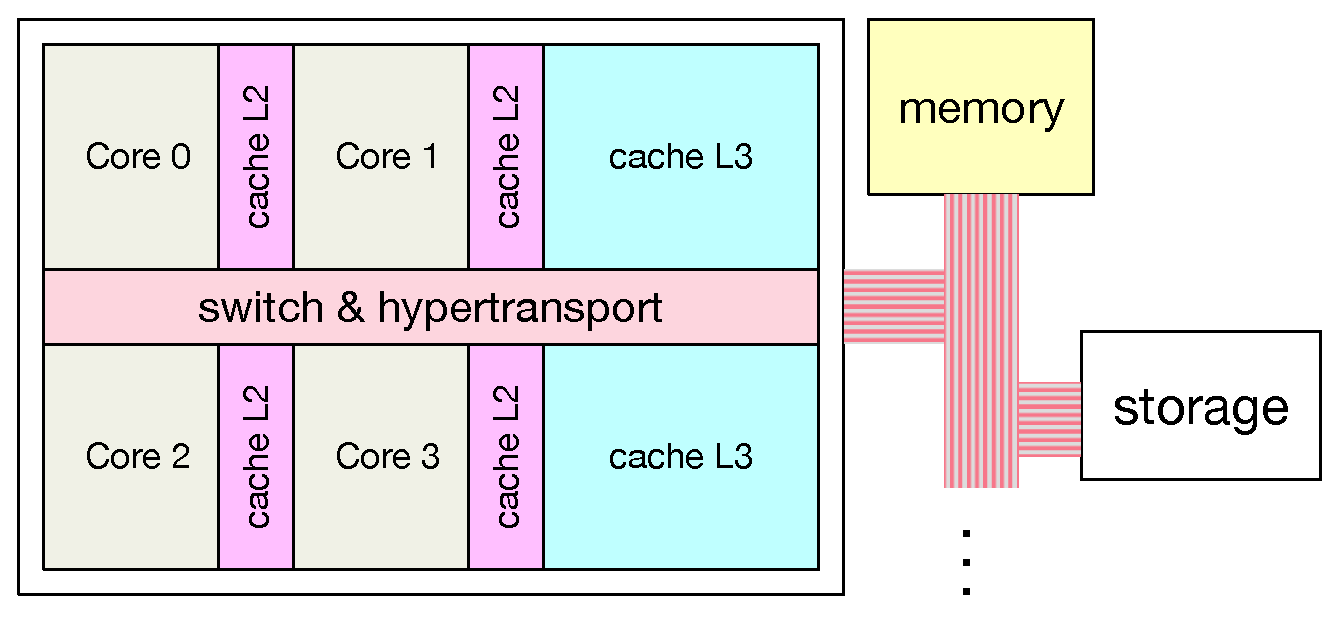
\includegraphics[width=1\textwidth]{figures/multicore.eps}
\end{column}
\end{columns}

Pros:
\begin{itemize}[-,noitemsep,topsep=-10pt]
\item \alert{Real parallelism}: as many DBMS processes as the number of cores running at the same time.
\item Can move a process from one core to another if needed.
\end{itemize}

\vskip1em

Cons:
\begin{itemize}[-,noitemsep,topsep=-10pt]
\item The BUS becomes a bottleneck!
\end{itemize}

\vskip1em

\footnotetext{\url{https://en.wikipedia.org/wiki/Multi-core_processor}}

\end{frame}


\begin{frame}

Modern ``single-box'' HPC servers have independent (multi-core) CPUs, each with its own memory, interconnected by a fast switch.

\vskip1em

\begin{center}
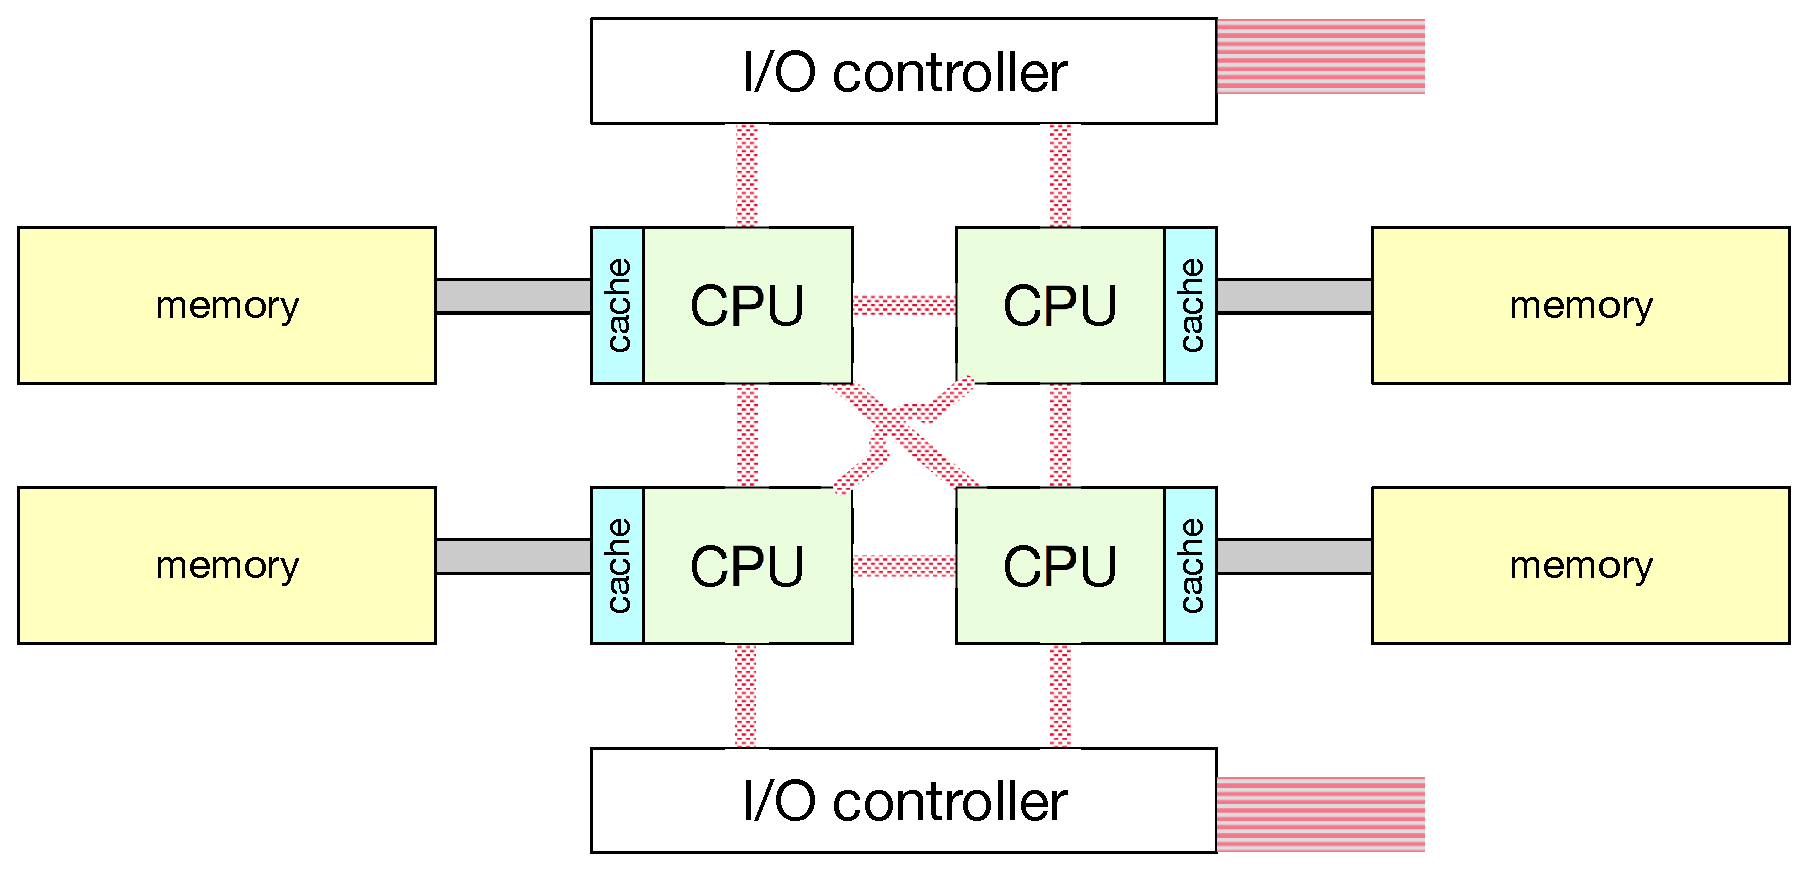
\includegraphics[width=0.75\textwidth]{figures/numa_architecture.eps}
\end{center}

\vskip1em

Processes on different CPUs can \alert{share memory}, but with a Non-Uniform Memory Access (\textbf{NUMA}\footnote{\url{https://en.wikipedia.org/wiki/Non-uniform_memory_access}}) cost: accessing local memory is cheaper.
\end{frame}


\begin{frame}{Shared Data Architectures}

When NUMA is not enough, we \alert{move \textbf{up}} to clusters of computers that shared only the data on disk:

\begin{center}
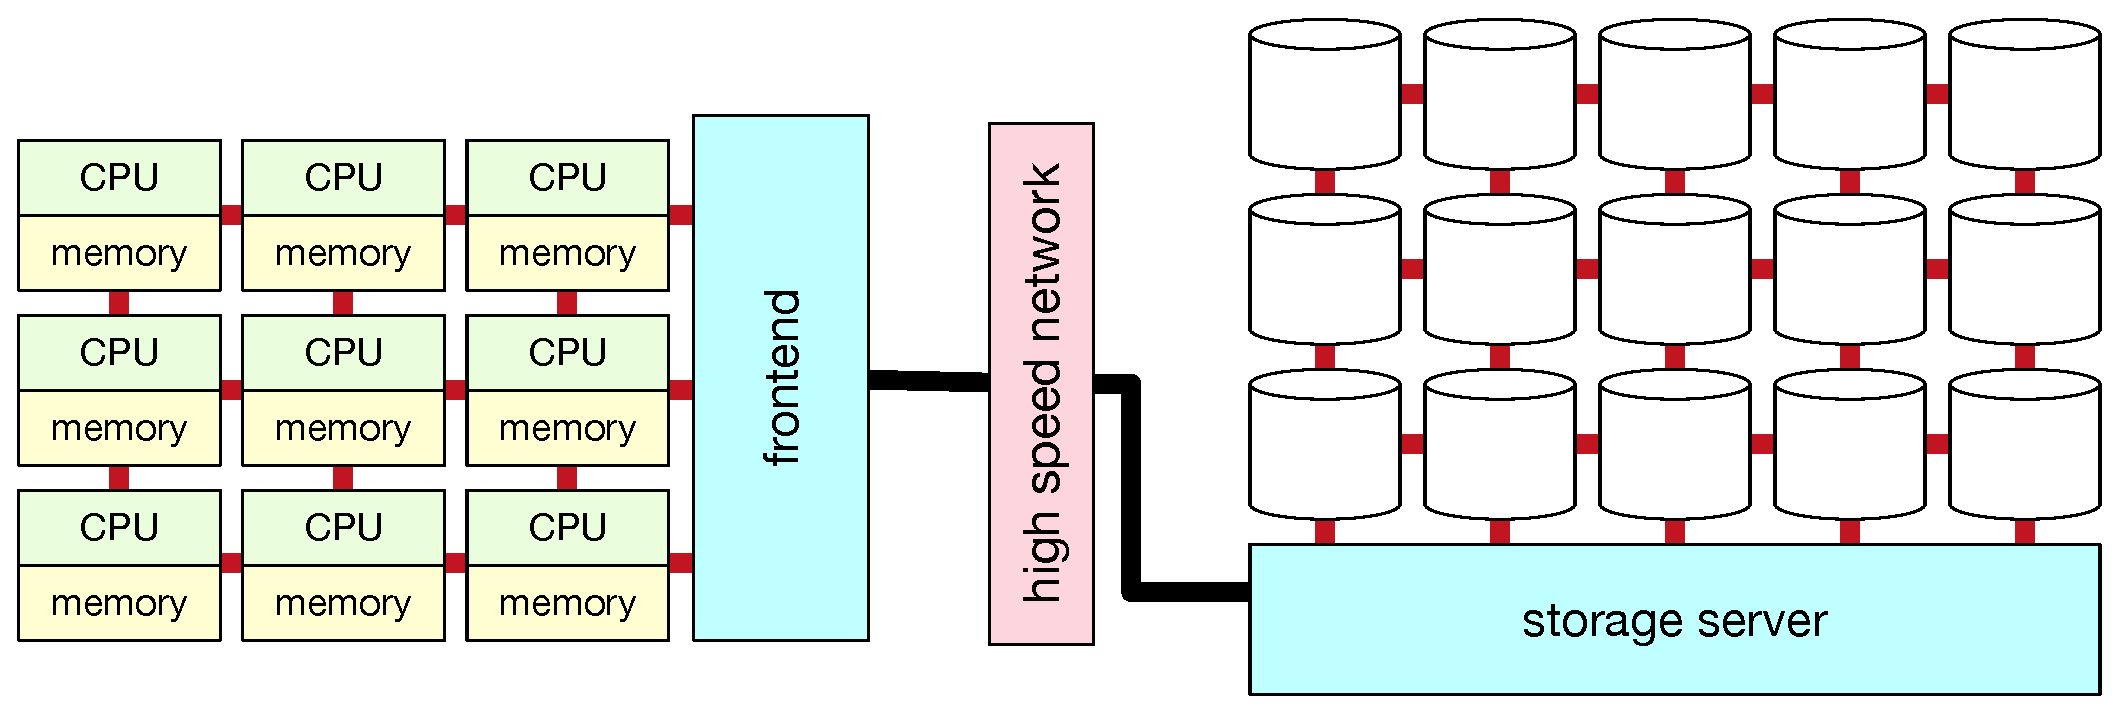
\includegraphics[width=0.75\textwidth]{figures/shared_disk_SAN.eps}
\end{center}

``Single-node DBMS'' in this architecture: transaction processes and DBMSs process run on separate nodes and communicate via a local network.

However, transferring data from the storage array becomes a bottleneck. A fast network can reach up to 5GB/s, but that would still mean 1 day to transfer 500 TB each way.

\end{frame}

\begin{frame}{Shared Nothing Architectures}

\begin{center}
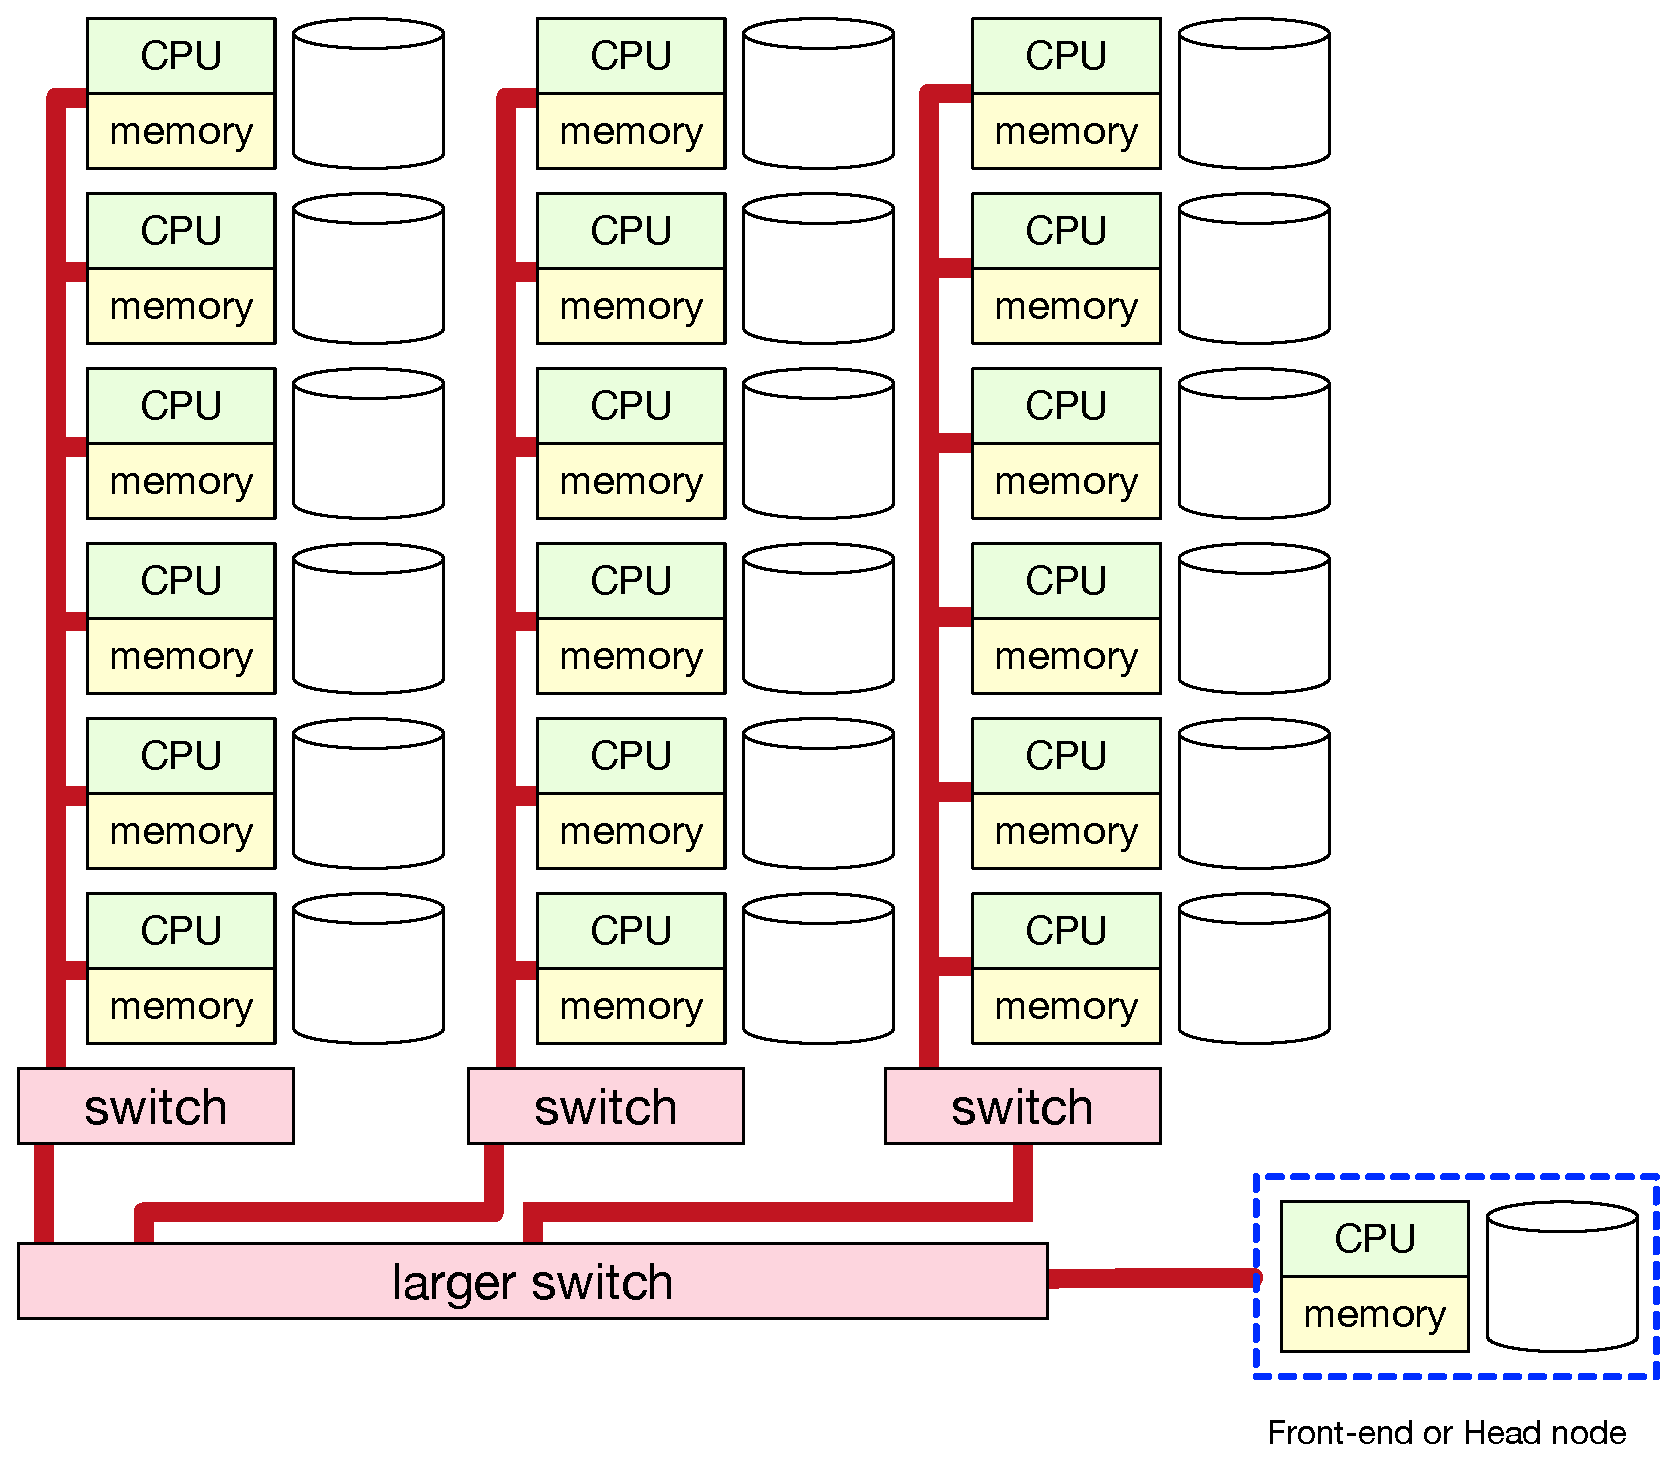
\includegraphics[width=0.75\textwidth]{figures/shared_nothing.eps}
\end{center}
\end{frame}

\begin{frame}{Why is Shared Nothing so Popular?}

Shared nothing architectures are made up of \alert{inexpensive} computing nodes, each with its own disk and memory (typically about \$1000 per node).

Shared nothing is ideal for \alert{scaling \textbf{out}} (instead of up): if you need more computing power, buy a few more computing nodes and hook them to the existing cluster.

\vskip1em

Shared nothing is great for \textbf{\alert{embarrassingly parallel}} workloads: spread the data among the nodes and run the same query (e.g., finding pages with links to \lstinline!ualberta.ca!) on every node at the same time.

\end{frame}

\begin{frame}{Virtualization and cloud computing}

Computing clouds are clusters of (shared-nothing) nodes that host a large number of virtual machines (VMs), each with their own OS.
\begin{itemize}[-]
\item Multiple VMs run simultaneously on the same physical node.
\item VMs can migrate across nodes (like processes migrate across processors).
\end{itemize}

\vskip1em


\end{frame}

\begin{frame}{Cloud Computing can Save (a lot!)}

Running an enterprise-scale datacenter incurs many costs:
\begin{itemize}[-,noitemsep]
\item Infrastructure: building maintenance, electricity, cooling, ...
\item Expertise: good IT staff costs a lot!
\end{itemize}

If the organization \textbf{under}-provisions (i.e., the IT infrastructure is too small), then it loses customers until it grows.

If the organization \textbf{over}-provisions (i.e., the IT infrastructure is too big), then it wastes money in maintenance cost.

\vskip1em

\begin{block}{Clouds $\approx$ Outsourced Infrastructure}
\alert{Main advantage}: let experts run the IT infrastructure and pay only for what you need (or what you use).
\end{block}
\end{frame}

\begin{frame}{Clouds continued}

\alert{Infrastructure as a Service} (IaaS):
\begin{itemize}[-,noitemsep,topsep=-10pt]
\item The cloud hosts ``bare bones'' VMs and the user installs their own OS and software stack
\end{itemize}

\alert{Platform as a Service}:
\begin{itemize}[-,noitemsep,topsep=-10pt]
\item The cloud offers self-managing VMs that implement a specific service
\begin{itemize}[-,noitemsep,topsep=-5pt]
\item email, word processing, other office applications
\item database services: MySQL, PostgreSQL, ...
\item document storage: MongoDB, CouchDB, ...
\item key/value ``data stores'': Bigtable, Cassandra, HBase, ...
\end{itemize}
\end{itemize}

\vskip1em

Google: {\footnotesize\url{https://cloud.google.com/products/\#databases}}

Amazon: {\footnotesize\url{https://aws.amazon.com/products/databases/}}
\end{frame}

\begin{frame}{Clouds bring economies of scale}

\begin{columns}[onlytextwidth]
\begin{column}{0.5\textwidth}
\begin{block}{\alert{Elasticity}}
Increasing/decreasing the number of VMs providing any service in response to changes in demand.
\end{block}

\begin{block}{Scaling \alert{Out}}
Growth by adding new physical nodes to cope with demand.
\end{block}
\end{column}
\qquad
\begin{column}{0.5\textwidth}
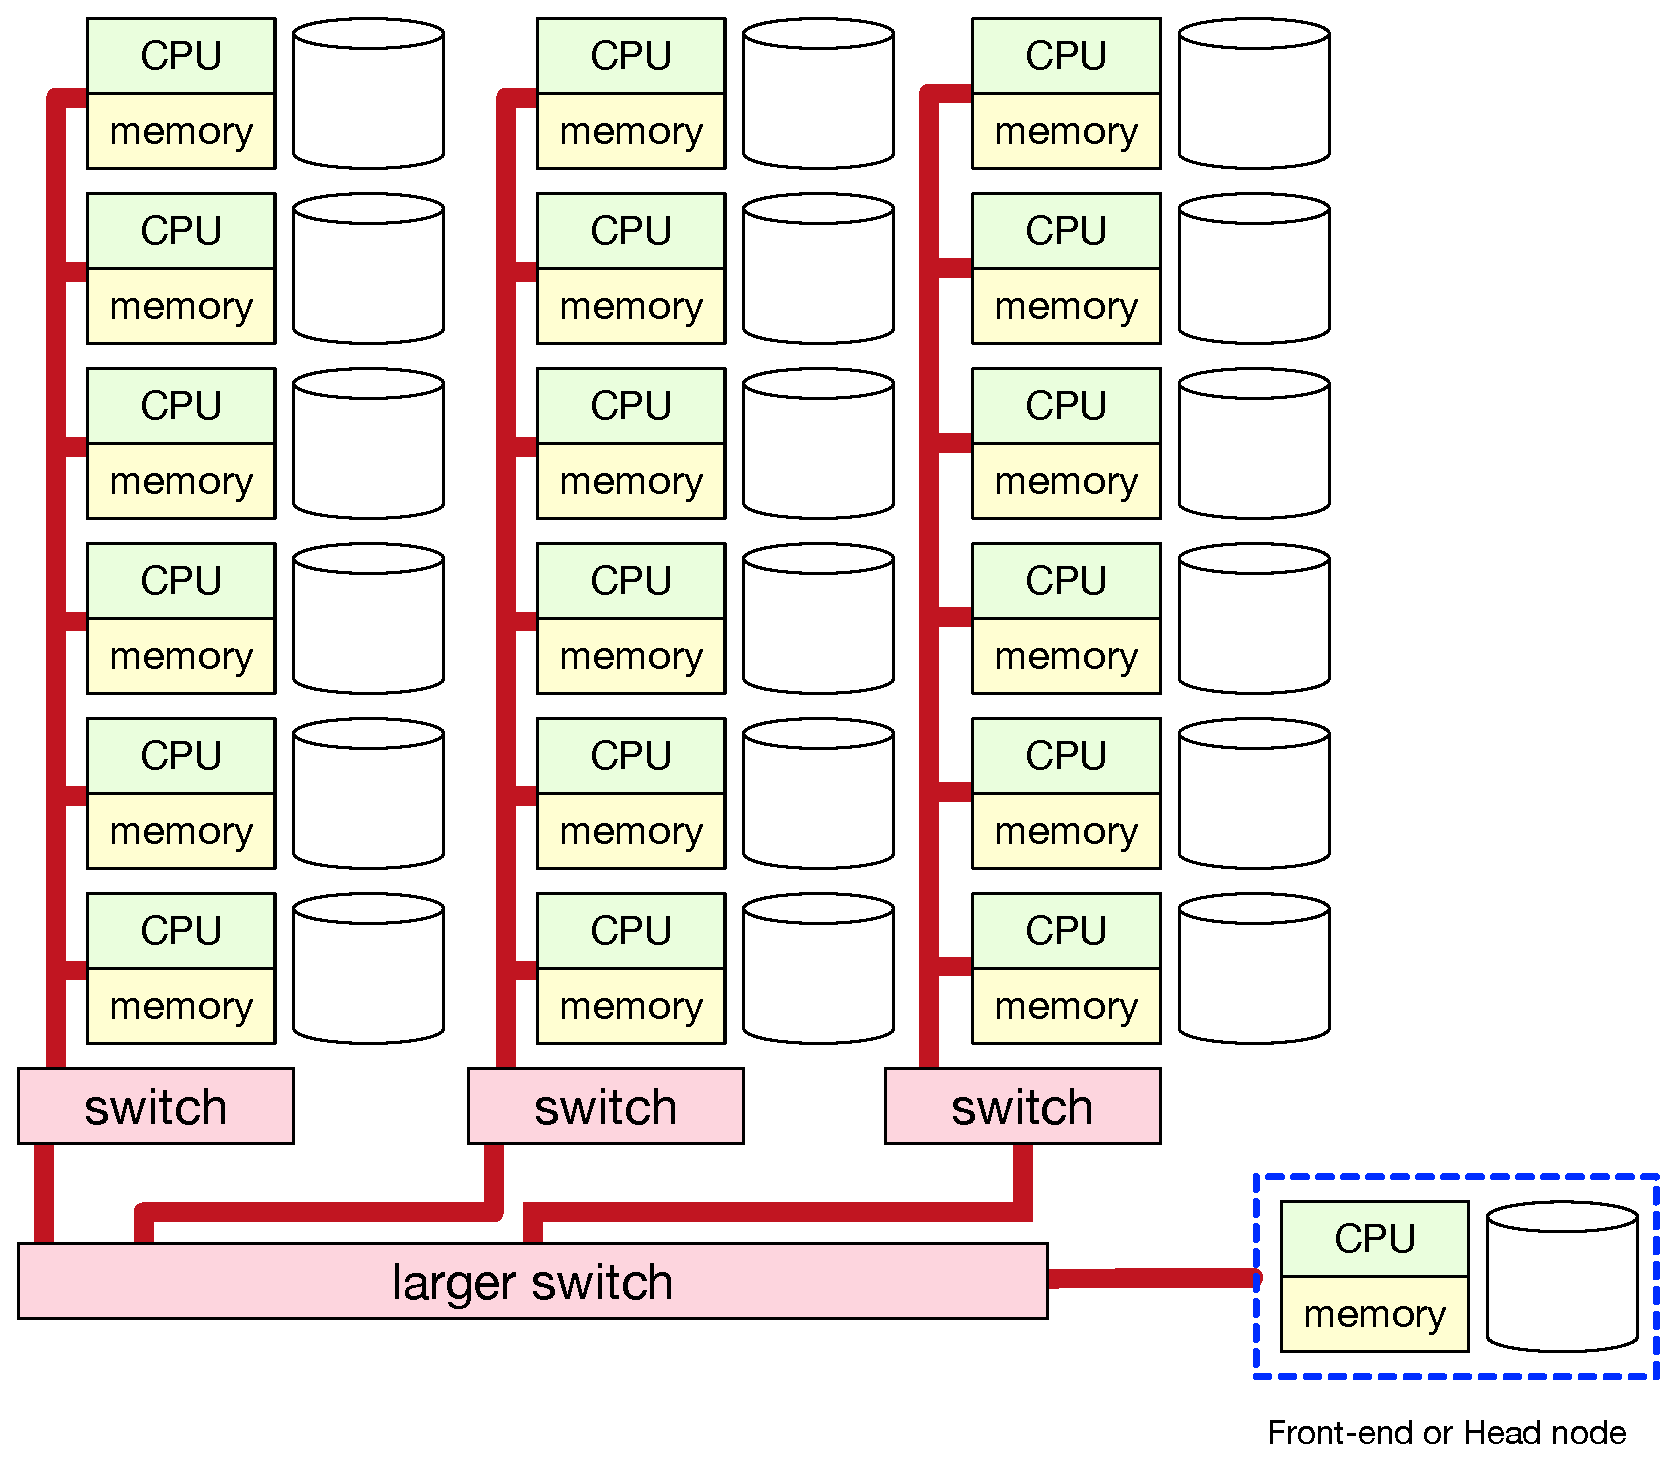
\includegraphics[width=0.9\textwidth]{figures/shared_nothing.eps}
\end{column}
\end{columns}

\vskip1em

\begin{block}{\alert{Multi-tenancy}}
Different clients have their VMs (or database services) running simultaneously on the same physical cluster.
\end{block}
\end{frame}


\begin{frame}{Redundancy is essential}
\begin{itemize}[-]
\item The cluster components (compute nodes and network connections) are inexpensive and will break at some point
\begin{itemize}[-,noitemsep]
\item Most clusters use commodity hardware; 
\item Google, Amazon and other massive IT companies have started to design their own custom compute nodes 
\end{itemize}
\item A data center with thousands of nodes will experience several node failures every day
\item \alert{Challenge \#1}: restarting the computation after each failure is not an option.... the computation model has to be \alert{\textbf{fault tolerant}}
\end{itemize}

\begin{block}{}
\alert{Redundancy} is one way of being fault tolerant: store the same on different compute nodes, across different cluster racks.
\end{block}
\end{frame}


\begin{frame}{Speedup and Scaleup}

\vskip1em

\begin{columns}[onlytextwidth]
\begin{column}{0.5\textwidth}
\centering
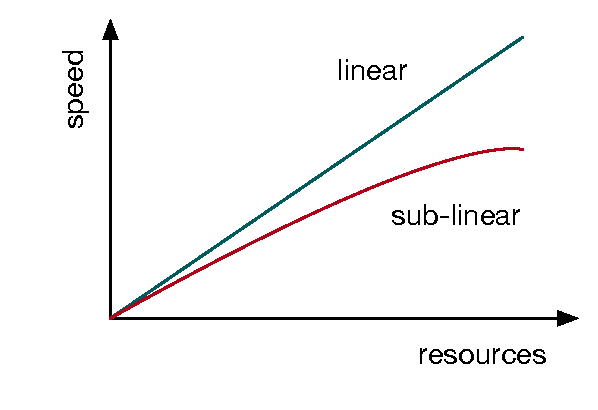
\includegraphics[width=\textwidth]{figures/speedup.eps}

Speedup
\end{column}
\begin{column}{0.5\textwidth}
\centering
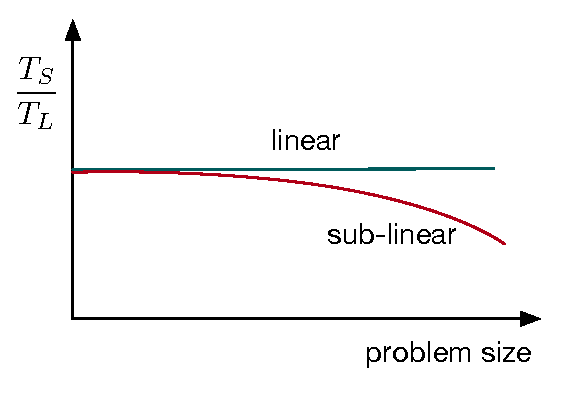
\includegraphics[width=\textwidth]{figures/scaleup.eps}

Scaleup
\end{column}
\end{columns}

\alert{\textbf{Speedup}} measures how much faster the system accomplishes a task as more computing resources are added.

\alert{\textbf{Scaleup}} takes into account the growth of the database. $T_S$ is the time it takes to complete the task on the ``small'' computer, while $T_L$ is the time on the ``large'' computer.

\end{frame}

\begin{frame}{HPC trade-offs}

A \alert{perfect high performance computer} (parallel or distributed) would have \textbf{linear speedup and scaleup}.

In practice this does not happen. The more components in a system, the more time is needed for them to coordinate amongst themselves.

\begin{block}{Example}
\begin{itemize}[-,noitemsep]
\item A DBMS log writer process responds faster to a server-side transaction process running on the same CUP instead of a process running on a different CPU or a different computer.
\end{itemize}
\end{block}

\textbf{Synchronizing independent processes takes time} proportional to the complexity of the computer. Also, we have to account for failures and build redundant checks (which also take time).
\end{frame}


\begin{frame}{Synchronization in DBMS workloads}

\textbf{Fact}: synchronization time grows with system complexity.

\alert{\textbf{Corollary}}: tasks that do not require synchronization show better speedup and scaleup.

\vskip1em


\begin{block}{\alert{\textbf{ACID transactions}} require a lot of synchronization}
\begin{itemize}[-,noitemsep,topsep=-10pt]
\item Atomicity requires logging.
\item Isolation requires transaction monitoring, locking, etc. which \underline{must be performed} by a single DBMS process.
\end{itemize}
\end{block}

A defining ``feature'' of many NoSQL systems that scale well is to not provide ACID transactions.

\end{frame}



\begin{frame}{Parallel vs Distributed Database}

In a single-node parallel database all the data and all DBMS processes reside in the same HPC computer, independently of architecture:

\vskip1em

\begin{columns}[onlytextwidth]
\begin{column}{0.3\textwidth}
\centering 
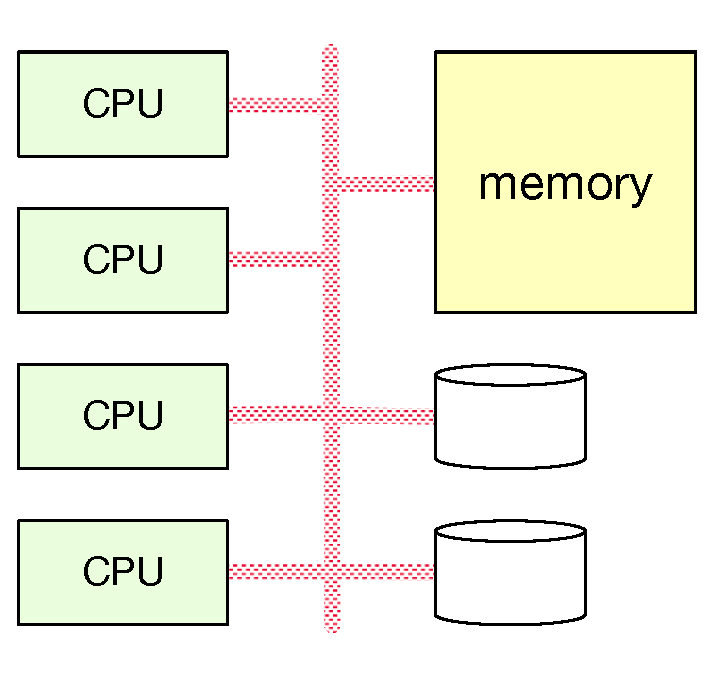
\includegraphics[width=0.75\textwidth]{figures/shared_memory_simplified.eps}

\footnotesize shared memory
\end{column}

\qquad \begin{column}{0.3\textwidth}
\centering 
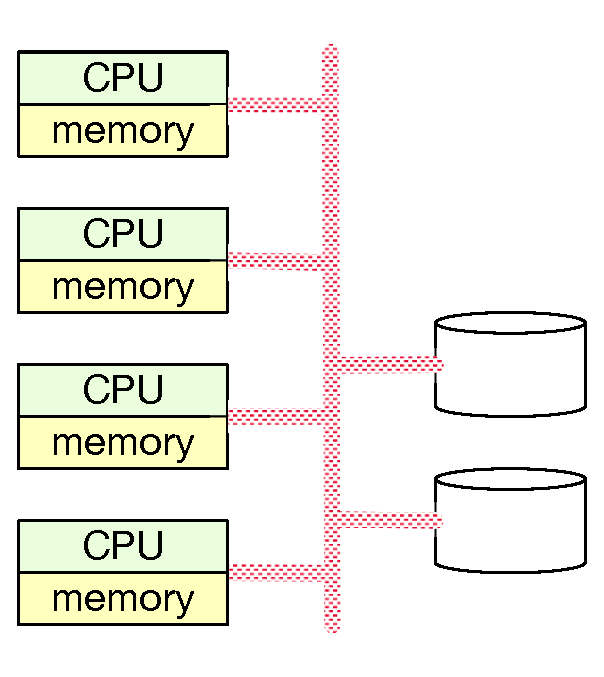
\includegraphics[width=0.75\textwidth]{figures/shared_disk_simplified.eps}

\footnotesize shared disk
\end{column}

\qquad \begin{column}{0.3\textwidth}
\centering 
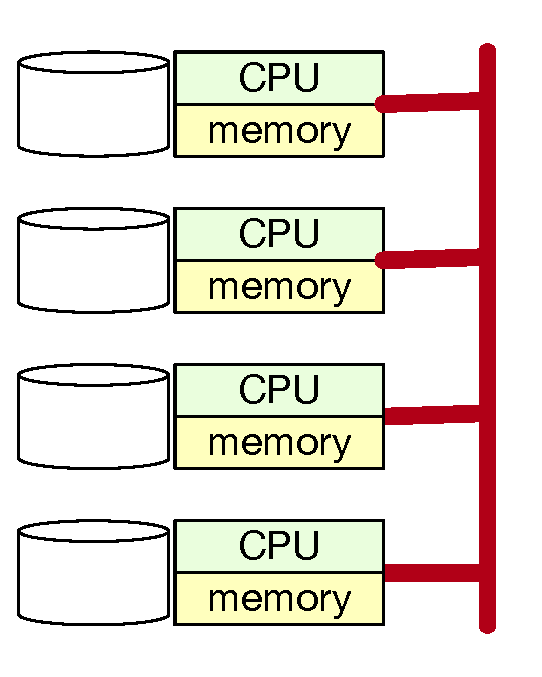
\includegraphics[width=0.75\textwidth]{figures/shared_nothing_simplified.eps}

\footnotesize shared nothing
\end{column}
\end{columns}

\vskip1em

A distributed database is one made of autonomous ``single-node'' databases. Typically, each database is located on a different data center (i.e., the nodes are geographically dispersed).

\end{frame}

\begin{frame}

We fill focus on shared-nothing clusters, as they are becoming the most popular (due to the cost benefits of cloud computing).

\vskip1em

Main questions about HPC NoSQL in the remaining of the notes:
\begin{itemize}[-]
\item What data management problems are shared nothing architectures best for?

\item What compromises do we make to handle more data or clients relative to what a single-node relational system offers?
\end{itemize}
\end{frame}

\section{Partitioned Table Stores}
%!TEX root = lec08_nosql.tex


%
%--------------------------------------------------------------------------------------------------------------
%

\begin{frame}{Data Partitioning}

\begin{columns}[onlytextwidth]
\begin{column}{0.5\textwidth}
Partitioning a table $R(a, b, c, d)$ within a cluster, can help \emph{balance} the storage and query/update workload across nodes.
\end{column}
\begin{column}{0.5\textwidth}
\begin{center}
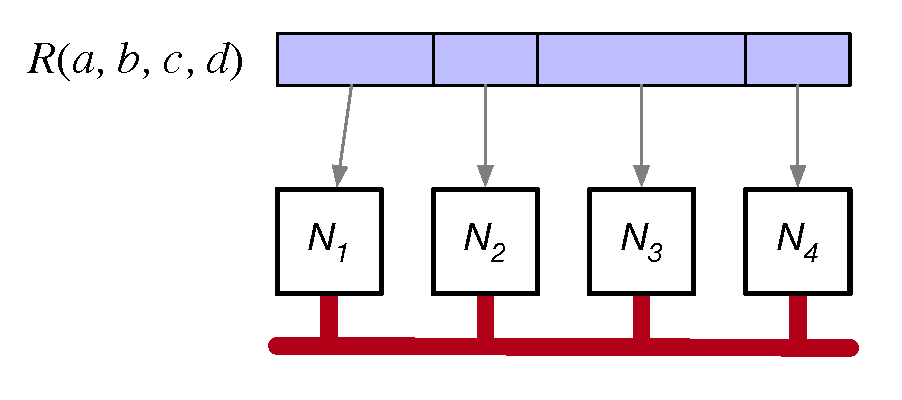
\includegraphics[width=\textwidth]{figures/table_partition_shared_nothing.eps}
\end{center}
\end{column}
\end{columns}

\vskip2em

\begin{itemize}[-,topsep=-10pt]
\item Based on \alert{ranges} of one or more partition attributes.\\
 Example, partition on $R(a)$: 
\(
\texttt{node}(t) = \left\{\begin{array}{cc}
                N_1 & t.a < k_1\\
                N_2 & k_1 \leq t.a < k_2\\
                ... & 
        \end{array}\right.
\)

\item Based on \alert{hashing} of one or more partition attributes.\\
 \(
 \texttt{node}(t) =  h(t.a) \bmod 4
 \)

\item In a round-robin fashion (i.e., tuples go to nodes based on the order they are inserted).
\end{itemize}
\end{frame}

%
%--------------------------------------------------------------------------------------------------------------
%

\begin{frame}{Cost of Finding a Tuple}

\begin{columns}[onlytextwidth]
\begin{column}{0.7\textwidth}
Recall that \blue{the costs of querying, deleting and updating a tuple all depended on the cost of finding a tuple} in t{e first place.}
\end{column}
\begin{column}{0.4\textwidth}
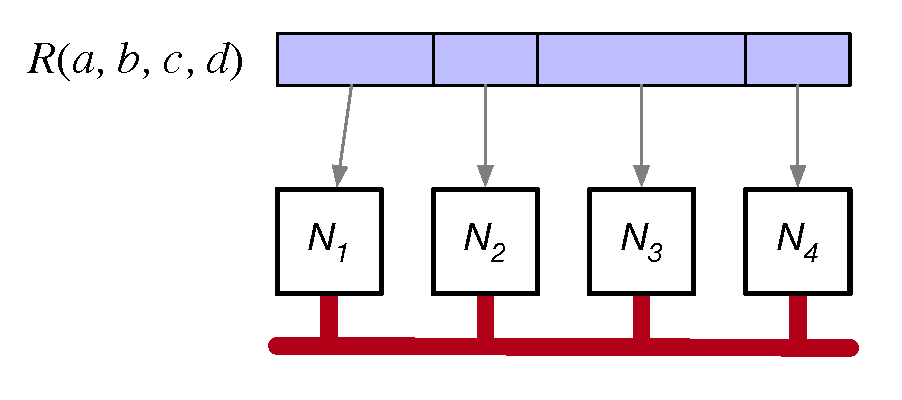
\includegraphics[width=0.75\textwidth]{figures/table_partition_shared_nothing.eps}
\end{column}
\end{columns}

\vskip1em

\alert{Cost of search based on $R(a) = v_1$}.
\begin{enumerate}[(1)]
\item Finding the node with the tuple:
\begin{itemize}[-,topsep=-10pt,noitemsep]
\item If $a$ is the partition attribute (range partition or hashing), we can quickly find the single node where the tuple is.
\item With round-robin partition \textbf{or} if $a$ is not the partition attribute, we need to search for the tuple in every node.
\end{itemize}
\item Performing the search in each node: $O(|R|)$ or $O(\log_k |R|)$ depending on whether there is an index on $a$.
\end{enumerate}

\end{frame}


%
%--------------------------------------------------------------------------------------------------------------
%

\begin{frame}{Data Distribution}

How many tuples will there be in each partition of $R$ into $R_1\cup R_2 \cdots\cup R_n$

\begin{itemize}[-,topsep=-0.5em]
\item With \textbf{round-robin}: \(T(R_i) = \dfrac{1}{N}\).
\item With \textbf{range partitioning} and with \textbf{hash partitioning}, it depends on how the distribution of the values of the partition attribute(s).
\begin{itemize}[-]
\item If the values of $R(a)$ are \blue{uniformly distributed} and $V(R,a) > N$, then \(T(R_i) = \dfrac{1}{N}\).
\item But what if they are not?
\end{itemize}
\end{itemize}
\end{frame}

%
%--------------------------------------------------------------------------------------------------------------
%

\begin{frame}

If the values of $R(a)$ are \alert{not uniformly distributed} then hashing and range partitioning will assign (possibly a lot) more tuples to a few nodes, causing the load in the cluster to be \textbf{unbalanced}.

\textbf{Ex:} suppose we partition \lstinline!Movie(title, year, imdb, director)! by year (left) or imdb score (right):

\vskip1em

\begin{columns}[onlytextwidth]
\begin{column}{0.5\textwidth}
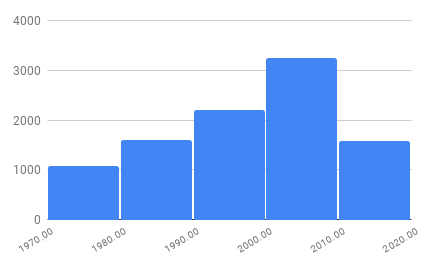
\includegraphics[width=\textwidth]{figures/histogram_year_skew.png}
\end{column}
\begin{column}{0.5\textwidth}
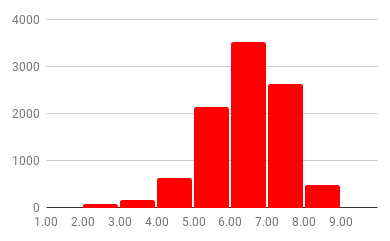
\includegraphics[width=\textwidth]{figures/histogram_imdb_skew.png}
\end{column}
\end{columns}

\begin{block}{\alert{Load imbalance is a problem}}
Nodes with more data perform \textbf{a lot more} work over time.
\end{block}
\end{frame}

%
%--------------------------------------------------------------------------------------------------------------
%

\begin{frame}{Virtual nodes}

One way to combat load imbalance is to add a level of indirection by using more \emph{virtual nodes} than real nodes:
\begin{itemize}[-,noitemsep,topsep=-9pt]
\item Use any partition scheme to assign tuples to virtual nodes.
\item Assign virtual nodes to real nodes in a round-robin fashion\footnote{The other two techniques would work as well.}.
\end{itemize}

\vskip2.5em

\begin{columns}[onlytextwidth]
\begin{column}{0.5\textwidth}
In effect, using \emph{virtual} nodes is the same as increasing the granularity of the data partitioning strategy. 
\vskip0.5em

Randomizing the assignment of virtual nodes to physical nodes 
\end{column}
\begin{column}{0.5\textwidth}
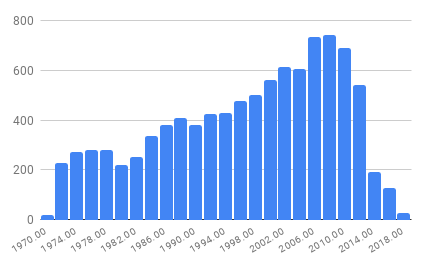
\includegraphics[width=\textwidth]{figures/histogram_year_skew_fine.png}
\end{column}
\end{columns}
\vspace*{-5pt}
\noindent balances out the workload of the physical nodes.

~
\end{frame}


%
%--------------------------------------------------------------------------------------------------------------
%

\begin{frame}
\vskip2em

\begin{columns}[onlytextwidth]
\begin{column}{0.5\textwidth}
Each virtual node corresponds to a narrower slice of the data.

\vskip1em

Each physical node is assigned multiple slices, in a way that the total load in each physical node is as egalitarian as possible.

\vskip1em

Ideally, each physical node should have

\[T(R)/N \text{ tuples.}\]
\end{column}

\qquad \begin{column}{0.5\textwidth}
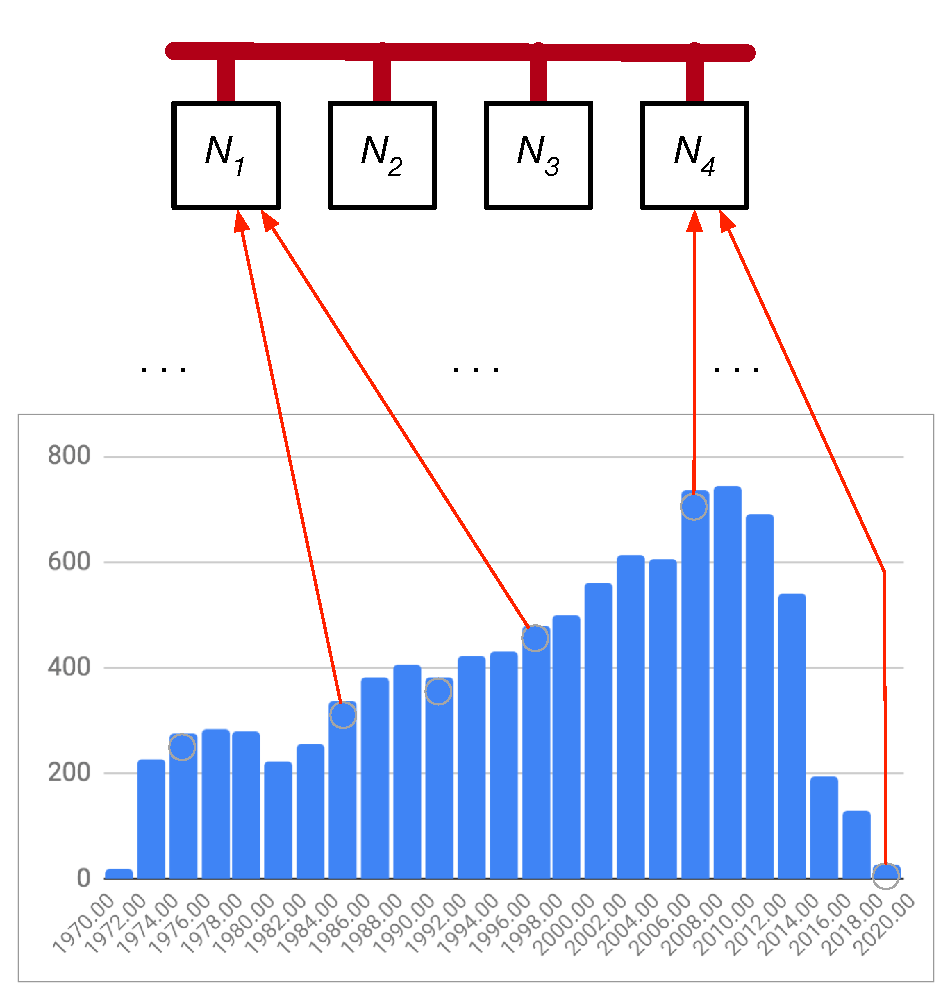
\includegraphics[width=\textwidth]{figures/virtual_node_rebalance.eps}
\end{column}
\end{columns}
\end{frame}

%
%--------------------------------------------------------------------------------------------------------------
%

\begin{frame}{Elasticity}

The use of virtual nodes to partition the data is consistent with the ``elastic nature'' of cloud computing:
\begin{itemize}[-]
\item When the cluster grows (i.e., new physical nodes are added), existing virtual nodes can be re-assigned and migrated.
\item Also, each ``slice'' of the data can be further divided into even narrower slices to help re-balance the load among physical nodes.
\end{itemize}
\end{frame}

%
%--------------------------------------------------------------------------------------------------------------
%

\begin{frame}{Replication, Redundancy and Availability}

Nodes in a cluster are \alert{expected to fail} often and without warning. 

A good way to \textbf{avoid data loss} is to keep multiple copies of the data, so that even the failure of a few nodes does not mean the entire table is lost.

\begin{center}
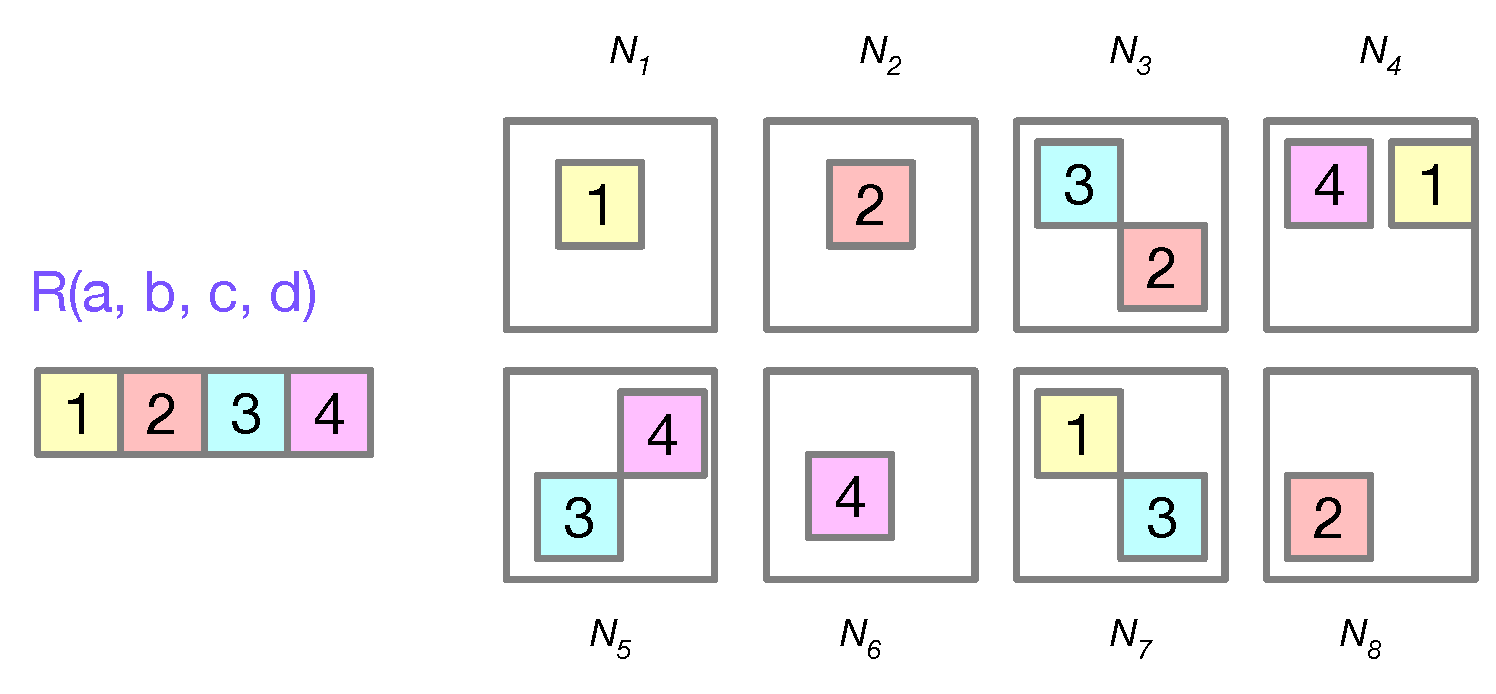
\includegraphics[width=0.75\textwidth]{figures/partitioned_table_redundancy.eps}
\end{center}

This also helps with query answering: always send request to read data to the nodes with least load.

\end{frame}


%
%--------------------------------------------------------------------------------------------------------------
%

\begin{frame}{Prototypical ``Table Store''}


The table is partitioned into \alert{tablets}, distributed and replicated across tablet servers. A \alert{directory} process, running in the \textbf{primary node} of the cluster, keeps a mapping between tablets to nodes. 

To increase availability and redundancy, directory process is replicated in multiple nodes, each running a \alert{data router} process.

\vskip1.5em

\begin{center}
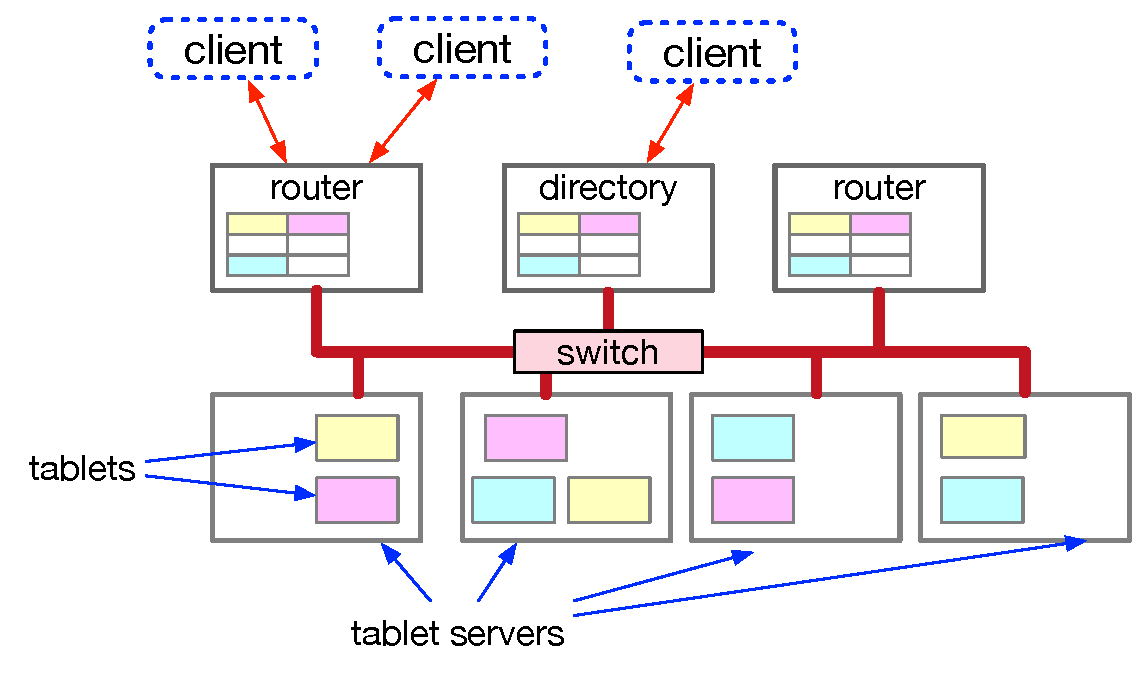
\includegraphics[width=0.75\textwidth]{figures/table_store_architecture.eps}
\end{center}

\end{frame}

%
%--------------------------------------------------------------------------------------------------------------
%

\begin{frame}

\begin{center}
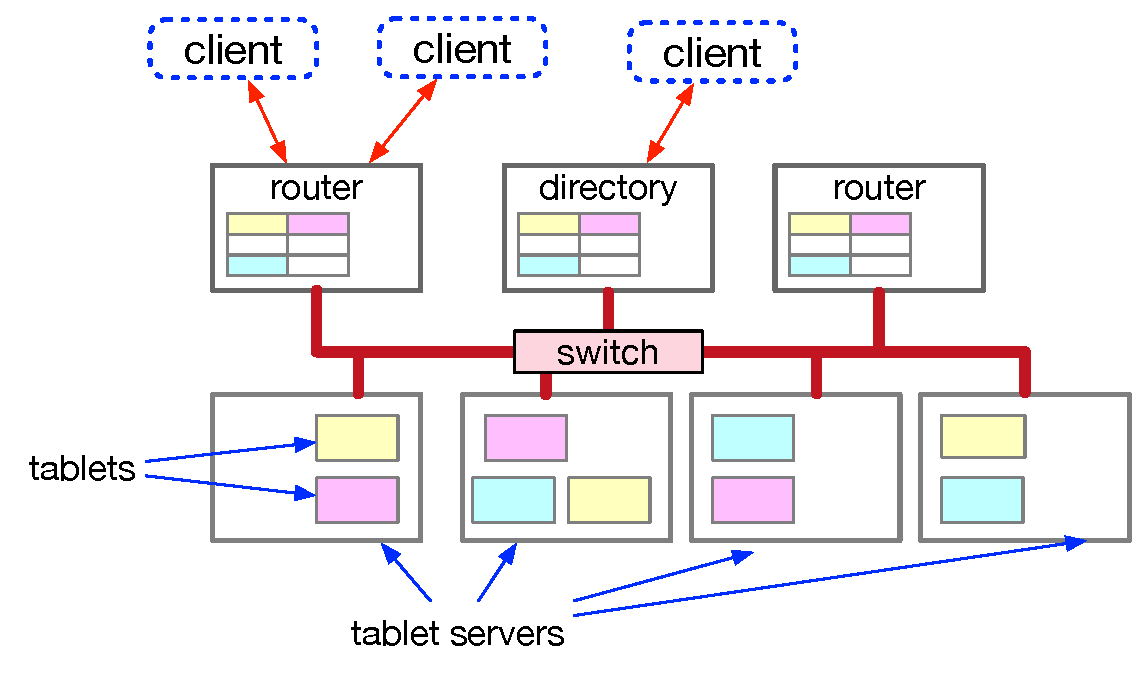
\includegraphics[width=0.75\textwidth]{figures/table_store_architecture.eps}
\end{center}

Small deployments will typically have a small number of physical nodes, each running multiple processes.

\begin{itemize}[-,noitemsep,topsep=-10pt]
\item Routing process: redirect requests based on partition attribute.
\item Data storage process: read/write operations on tuples.
\item Load re-balancing process.
\item Query/transaction execution process!
\end{itemize}
\end{frame}

%
%--------------------------------------------------------------------------------------------------------------
%

\begin{frame}{Updating the data}

Inserting new tuples requires choosing a primary tablet to hold the tuple and updating the directory accordingly.

To delete a tuple or to modify a non-partition attribute of a tuple, we:

\begin{enumerate}[(1),noitemsep,topsep=-5pt]
 \item Find the tablet with the \textbf{primary} copy of the tuple.
 \item Perform the update/deletion.
 \item Synchronize \alert{all replicas} of that partition.
 \end{enumerate} 

\vskip1em

Updating the partition attribute(s) is often implemented as deleting the tuple followed by an insertion of the ``modified'' one.
\end{frame}


%
%--------------------------------------------------------------------------------------------------------------
%
\begin{frame}{Synchronization}

Recall that in these systems data loss is prevented by having each tuple stored in multiple places. 

Which means we need to replicate every insertion and every update in the primary tablet to its replicas.

\vskip1em

\begin{block}{How do we ensure the replicas are \blue{synchronized}?}
\begin{itemize}[-,noitemsep]
\item \alert{Two-phase Commit (2PC) protocol}\footnotemark ensures synchronous and atomic updates across replicas.
\item Persistent-messaging implements a more relaxed, \textbf{eventual}, consistency model.
\end{itemize}
\end{block}

% \vskip1em

\footnotetext{\url{https://en.wikipedia.org/wiki/Two-phase_commit_protocol}}

\end{frame}

%
%--------------------------------------------------------------------------------------------------------------
%

\begin{frame}{Why do we need synchronization again?}

Synchronization is necessary (in single-node or multi-node systems) to ensure that transactions are atomic and durable and to ensure that the transaction schedule is conflict-serializable.

\vskip1em

In other words, \alert{synchronization is needed if we want ACID transactions}.

\vskip1em

\begin{block}{Not all applications need synchronization though...}

As we will discuss (soon) some applications can tolerate data inconsistencies as long as they can be (eventually) detected and corrected.

\vskip1em

\alert{\textbf{Trade-off:}} give up consistency to gain in speed.
\end{block}

\end{frame}



\section{Consistency and Transaction Processing}
%!TEX root = lec08_nosql.tex

%
%--------------------------------------------------------------------------------------------------------------
%

\begin{frame}{Distributed Transactions}

Nodes in the cluster execute two kinds of transactions:

\begin{itemize}[-,noitemsep,topsep=-10pt]
\item \textbf{\alert{Local transactions}} only read/write data on the node running the transaction.
\item \textbf{\alert{Global transactions}} read/write data on multiple nodes.
\end{itemize}

\vskip2em

\begin{columns}[onlytextwidth]
\begin{column}{0.55\textwidth}
The \textbf{transaction coordinator} synchronizes the individual (local) transactions running on different nodes via the network.
\end{column}
\begin{column}{0.45\textwidth}
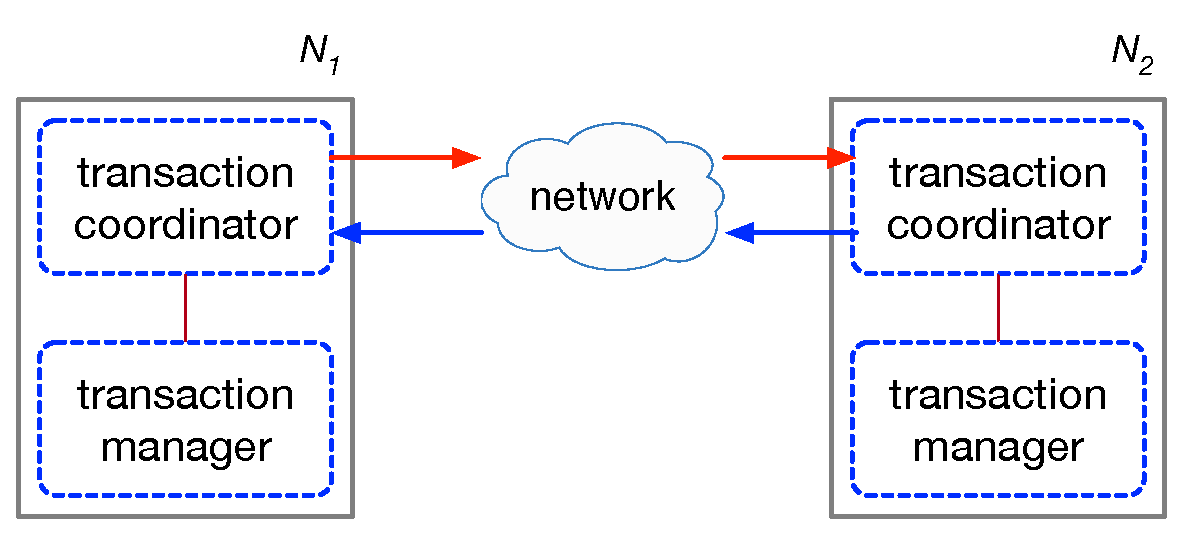
\includegraphics[width=1\textwidth]{figures/transaction_coordination.eps}
\end{column}
\end{columns}

\vskip1em

The \textbf{transaction manager} is responsible for logging and concurrency control \alert{only within the node where it runs}.

\end{frame}

%
%--------------------------------------------------------------------------------------------------------------
%

\begin{frame}{Two-Phase Commit Protocol (2PC) without failures}

2PC ensures transactions commit \textbf{if and only} all replicas are consistent. Assume node $N_1$ (with transaction coordinator $\mathit{TC}_1$) starts transaction $T_x$.

\begin{enumerate}[(1),noitemsep,topsep=-10pt]
\item $\mathit{TC}_1$ periodically sends messages to all other $\mathit{TC}_i$ that are affected by the transaction, e.g., so that they write the new values to their logs, etc.

\item \textbf{\alert{Phase 1}}: starts when the transaction is ready to commit; $\mathit{TC}_1$ writes \lstinline[style=cmput391]!<prepare Tx>! to its log, flushes its log, and sends a \textbf{prepare} message to all other $\mathit{TC}_i$ involved.\\
~~ All replicas write \lstinline[style=cmput391]!<ready Tx>! to their log and respond to $\mathit{TC}_1$ that they are ready.

\item \textbf{\alert{Phase 2}}: starts when $\mathit{TC}_1$ gets the ok from \underline{all replicas}, it writes \lstinline[style=cmput391]!<commit Tx>! to its log, flushes its log, and sends a commit message to all other $\mathit{TC}_i$.
\end{enumerate}
\end{frame}


%
%--------------------------------------------------------------------------------------------------------------
%

\begin{frame}{2PC timeline}
\begin{center}
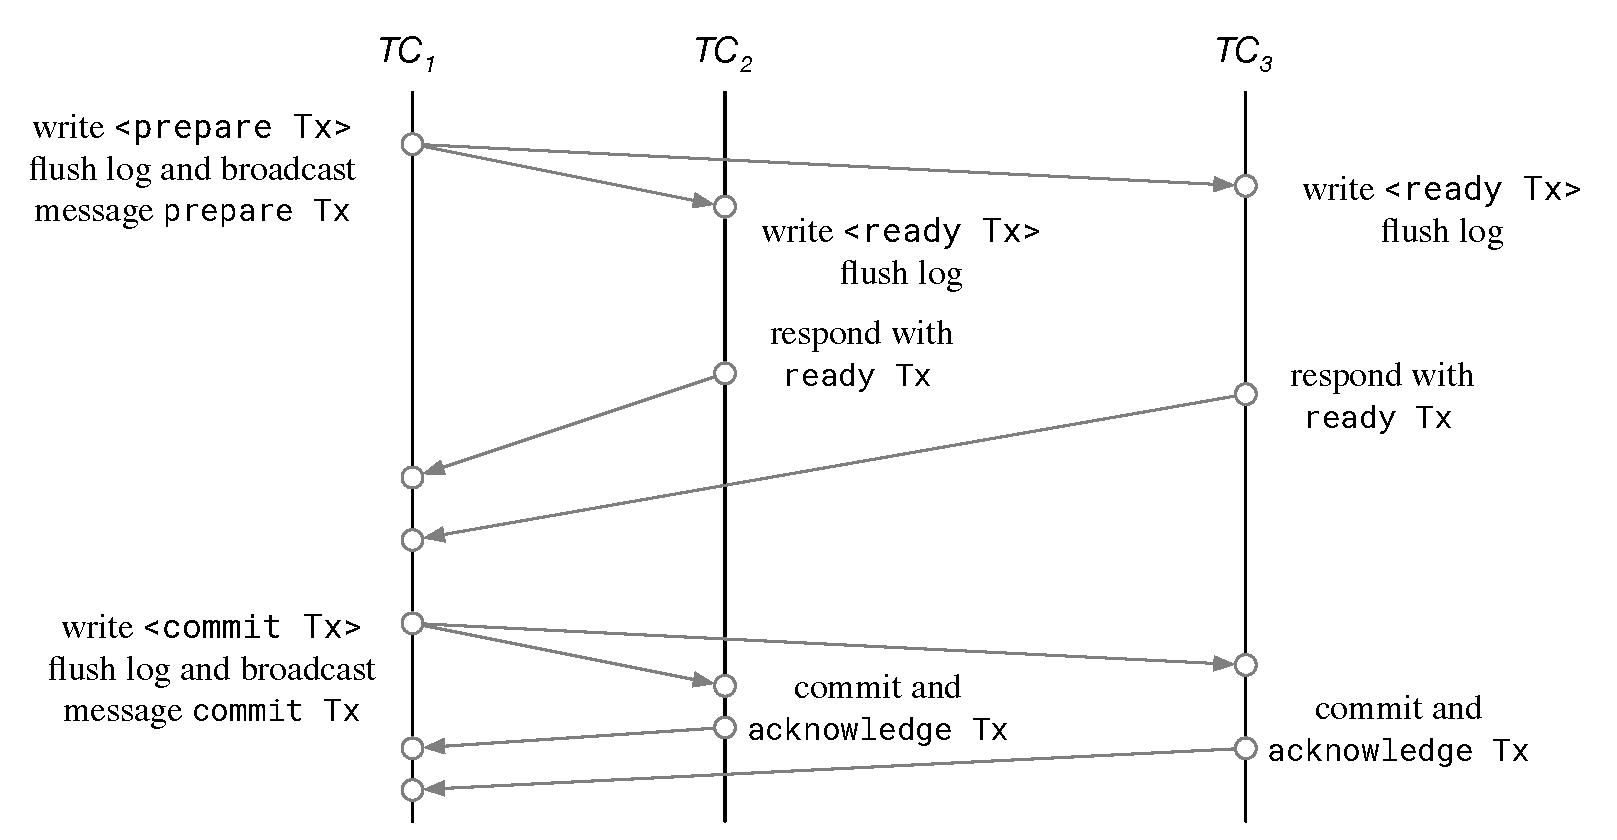
\includegraphics[width=\textwidth]{figures/2PC_example.eps}
\end{center}

$\mathit{TC}_2$ and $\mathit{TC}_3$ are the replicas of $\mathit{TC}_1$
\end{frame}

%
%--------------------------------------------------------------------------------------------------------------
%

\begin{frame}{2PC: correctness}
Rule \#1: $\mathit{TC}_1$ will only start the attempt to commit if all replicas respond with a \lstinline[style=cmput391]!<ready Tx>! message.

 If a replica cannot commit or does not respond after some time limit, the transaction is aborted and all replicas are notified to abort.

\vskip1.5em

Rule \#2: $\mathit{TC}_1$ knows all replicas are synchronized once they all respond with a \lstinline[style=cmput391]!<acknowledge Tx>! message.

\vskip1.5em

The protocol deals with different kinds of failures both in the coordinator node or in the replica node.
\end{frame}


%
%--------------------------------------------------------------------------------------------------------------
%

\begin{frame}{2PC: replica failure}

If the coordinator $\mathit{TC}_1$ detects that replica node $N_j$ failed \textbf{before} responding with \lstinline[style=cmput391]!<ready Tx>!, it assumes the replica is not ready and aborts the transaction everywhere, and no inconsistencies arise.

\vskip2em

If the coordinator $\mathit{TC}_1$ detects that replica node $N_j$ failed \textbf{after} responding with \lstinline[style=cmput391]!<ready Tx>!, it continues with the protocol with the other replicas, ignoring the node failure.

Once the failed replica $N_j$ is back up, it performs a crash recovery algorithm (next slide).
\end{frame}

%
%--------------------------------------------------------------------------------------------------------------
%

\begin{frame}{2PC: crash recovery --- replica}

Upon restart, replica $N_j$ checks its log to undo/redo transactions almost as in the single-node case (recall undo/redo logging from before). For each transaction $T_x$ in the log:

\begin{itemize}[-,noitemsep,topsep=-5pt]
\item If \lstinline[style=cmput391]!<commit Tx>! is found in the log, \textbf{redo} $T_x$.
\item If \lstinline[style=cmput391]!<abort Tx>! is found in the log, \textbf{undo} $T_x$.
\item If only \lstinline[style=cmput391]!<ready Tx>! is found in the log, then the replica must \alert{consult the transaction coordinator} $\mathit{TC}_1$ to figure out the if the transaction committed or aborted.
\begin{itemize}[-,topsep=-10pt]
\item If the coordinator is unreachable, $N_j$ queries all other replicas to check the status of the transaction.
\item Until then, $N_j$ \textbf{neither} commits nor aborts.
\end{itemize}
\item If not even \lstinline[style=cmput391]!<ready Tx>! is in the log, the replica did not respond (and the transaction has been aborted by the coordinator), so the replica aborts the transaction.
\end{itemize}
\end{frame}

%
%--------------------------------------------------------------------------------------------------------------
%

\begin{frame}{2PC: coordinator failure}

If the coordinator fails or becomes unavailable during the execution of the transaction, the replicas continue executing the transaction to the extent possible:
\begin{itemize}[-,noitemsep,topsep=-5pt]
\item If at least one replica wrote \lstinline[style=cmput391]!<commit Tx>! to its log, then all active replicas proceed to commit the transaction.
\item If an active replica wrote \lstinline[style=cmput391]!<abort Tx>!, then all active replicas must abort.
\item If at least one replica \alert{does not} have \lstinline[style=cmput391]!<ready Tx>! in its log, the coordinator cannot have started the commit phase. In this case, the replicas assume the coordinator decided to abort (based on timeout) and they all abort.
\item If all replicas have only the \lstinline[style=cmput391]!<ready Tx>! in their log, then the replicas must \alert{wait for the transaction coordinator} $\mathit{TC}_1$ to figure out the if the transaction committed or aborted.
\end{itemize}
\end{frame}

%
%--------------------------------------------------------------------------------------------------------------
%

\begin{frame}{2PC: crash recovery --- coordinator}

The crash recovery for the coordinator is identical to that of a replica $N_j$:

\begin{itemize}[-,noitemsep,topsep=-5pt]
\item Redo and commit transactions marked \lstinline[style=cmput391]!<commit Tx>! the log.
\item Undo and abort transactions marked \lstinline[style=cmput391]!<abort Tx>! in the log.
\item Consult the replicas about transactions marked \lstinline[style=cmput391]!<ready Tx>! in the log.
\item If not even \lstinline[style=cmput391]!<ready Tx>! is in the log, the replicas did not respond before the crash, and everyone decided to abort the transaction.
\end{itemize}
\end{frame}


%
%--------------------------------------------------------------------------------------------------------------
%

\begin{frame}{Network partition and delayed transactions}

\vskip2em

\begin{columns}[onlytextwidth]
\begin{column}{0.55\textwidth}

A severe network failure might partition the system into two disconnected subsystems.

\vskip1em

The 2PC protocol dictates how the coordinator and the replicas behave if the failure happens during the execution of a transaction.
\end{column}
\qquad\begin{column}{0.45\textwidth}
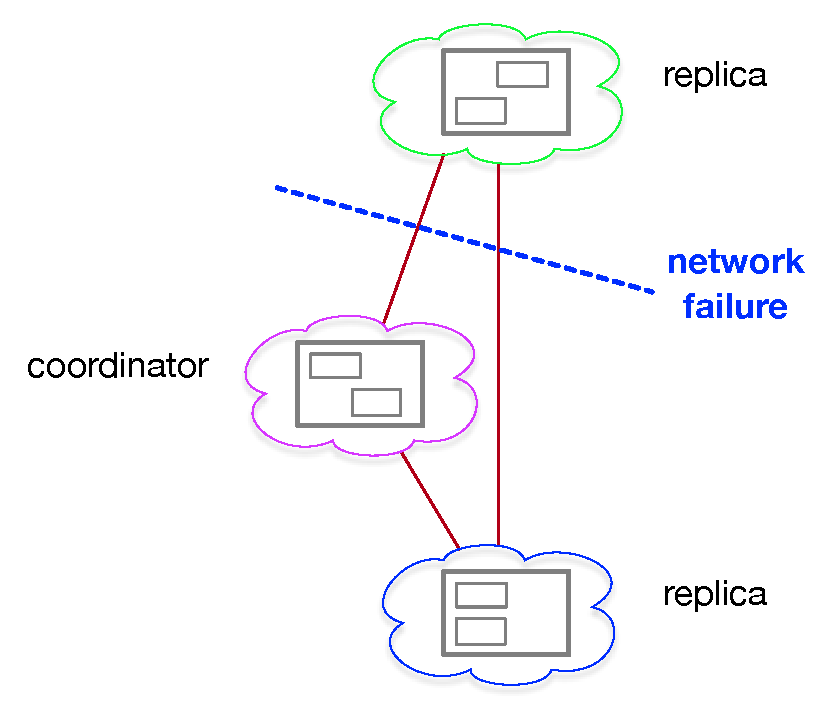
\includegraphics[width=1\textwidth]{figures/network_failure_partition.eps}
\end{column}
\end{columns}

\vskip1em

However, can the same query have a different answer depending on the node it is issued?

Also, should new transactions be accepted while the network is partitioned?

\end{frame}


%
%--------------------------------------------------------------------------------------------------------------
%

\begin{frame}

\vskip2em

\begin{columns}[onlytextwidth]
\begin{column}{0.55\textwidth}

Example: if the isolated replica could not decide whether or not to commit or abort a transaction $T_x$, it \textbf{cannot} accept new transactions that use data written by $T_x$!

\vskip1em

But what about the other nodes in the ``other half'' of the system?
\end{column}
\qquad\begin{column}{0.45\textwidth}
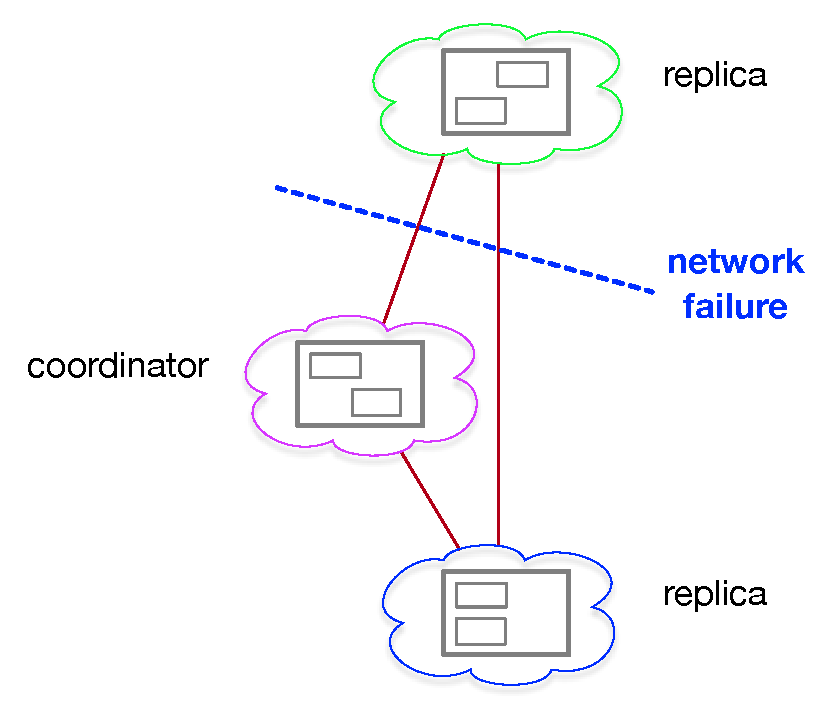
\includegraphics[width=1\textwidth]{figures/network_failure_partition.eps}
\end{column}
\end{columns}

\vskip1em

What if the network failure may last for a long time? 
\begin{itemize}[-,noitemsep]
\item Should the system stop accepting transactions? 
\item What about queries?
\end{itemize}
\end{frame}

%
%--------------------------------------------------------------------------------------------------------------
%

\begin{frame}{Accepting Transactions in a Partitioned System}


\begin{columns}[onlytextwidth]
\begin{column}{0.55\textwidth}

\begin{block}{The \alert{blocking} problem}
A node isolated from the rest of the network it may not know if a transaction committed or aborted, preventing it from accepting new transactions (e.g., to avoid uncommitted reads).
\end{block}

\end{column}
\qquad\begin{column}{0.45\textwidth}
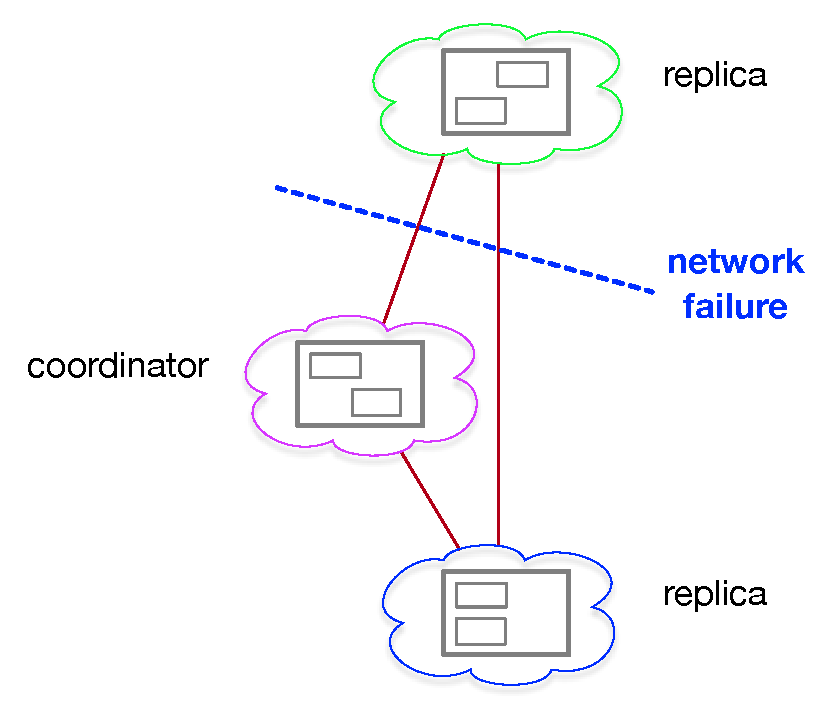
\includegraphics[width=1\textwidth]{figures/network_failure_partition.eps}
\end{column}
\end{columns}

\vskip0.75em

But distributing the data was meant to bring \textbf{\alert{high availability}}. Instead, the whole system becomes unavailable when there is a failure somewhere else.

\alert{High Availability} and \textcolor{blue}{Data Consistency} are conflicting goals...
\end{frame}


%
%--------------------------------------------------------------------------------------------------------------
%

\begin{frame}{Eventual Consistency With Majority Locking}

\vskip2em

\begin{columns}[onlytextwidth]
\begin{column}{0.65\textwidth}
One way to allow the system to tolerate node or network failures is to allow a transaction $T_1$ to write a database element \alert{A} if it can acquire locks on the (simple) majority of the nodes with copies of \alert{A}.

\vskip1em

\textbf{Timestamps} (agreed upon at locking time) are used to record the version of \alert{A} that is written.

\vskip1em

After the update commits the system becomes inconsistent: different nodes have different ``most recent'' values of the same element.
\end{column}
\begin{column}{0.3\textwidth}
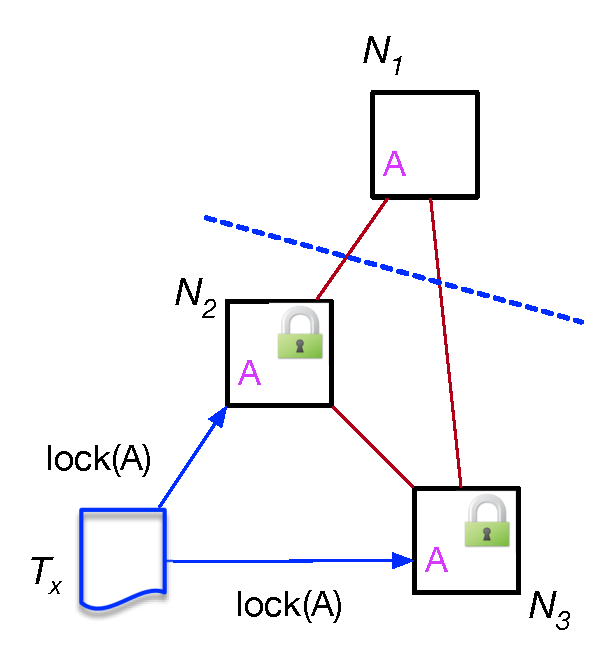
\includegraphics[width=\textwidth]{figures/majority_locking_A.eps}

\vskip1em

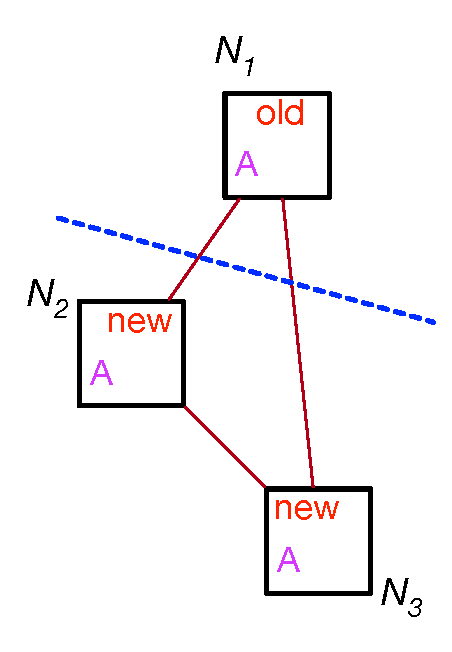
\includegraphics[width=0.75\textwidth]{figures/majority_inconsistent_A.eps}
\end{column}
\end{columns}
\end{frame}

%
%--------------------------------------------------------------------------------------------------------------
%

\begin{frame}

\begin{columns}[onlytextwidth]
\begin{column}{0.55\textwidth}
Inconsistent data can be detected in many ways:
\begin{itemize}[-,noitemsep,topsep=-5pt]
 \item A node with a copy of \alert{A} re-joins the network after a failure and asks its peers for missed transactions.
 \item Another node requests \alert{A} from all copies and gets inconsistent answers.
\end{itemize}
\end{column}
\begin{column}{0.4\textwidth}
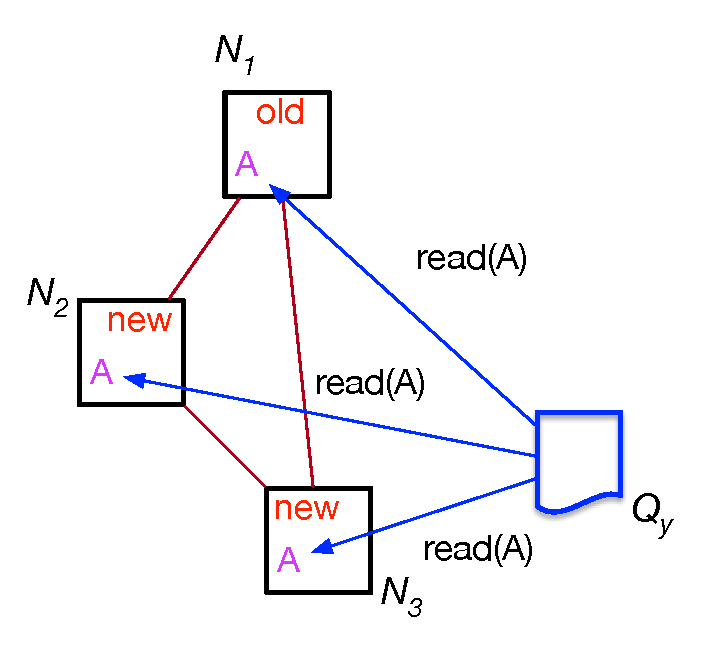
\includegraphics[width=1.1\textwidth]{figures/majority_read_all.eps}
\end{column}
\end{columns}

In summary, majority voting ensures the system remains available during the failure of a node, but incurs too many reads to work well.

\end{frame}

%
%--------------------------------------------------------------------------------------------------------------
%

\begin{frame}{The CAP ``Theorem''}

Although this is not a formal statement, it is generally accepted that no distributed database system that enforces \alert{ACID} transactions can achieve these three properties \textbf{simultaneously}:
\begin{itemize}[-,noitemsep,topsep=-10pt]
\item \alert{\textbf{C}}onsistency: all replicas have the same value.
\item \alert{\textbf{A}}vailability: the system accepts transactions at any time.
\item \alert{\textbf{P}}artition tolerance: the system operates normally even under a network partition failure.
\end{itemize}

\vskip1.5em

Instead of ACID, NoSQL systems are \textcolor{blue}{BASE}:
\begin{itemize}[-,noitemsep,topsep=-10pt]
\item \textcolor{blue}{\textbf{BA}}sically available: it works as long as the majority of the replicas are up.
\item \textcolor{blue}{\textbf{S}}oft state: inconsistencies are time-stamped.
\item \textcolor{blue}{\textbf{E}}ventually consistent: replicas do synchronize after a while.
\end{itemize}
\end{frame}

%
%--------------------------------------------------------------------------------------------------------------
%

\begin{frame}{Synchronization across data centers}

\vskip2em

\begin{columns}[onlytextwidth]
\begin{column}{0.6\textwidth}
Many applications require the data to be \alert{\textbf{distributed}} across geographically dispersed data centers to reduce the chance of critical data loss due to catastrophic failures in one location (e.g., fire in one data center).

\vskip0.75em

The 2PC protocol works on these systems as well, although network latency and connectivity can introduce significant delays in replica synchronization.

\end{column}
\qquad\begin{column}{0.4\textwidth}
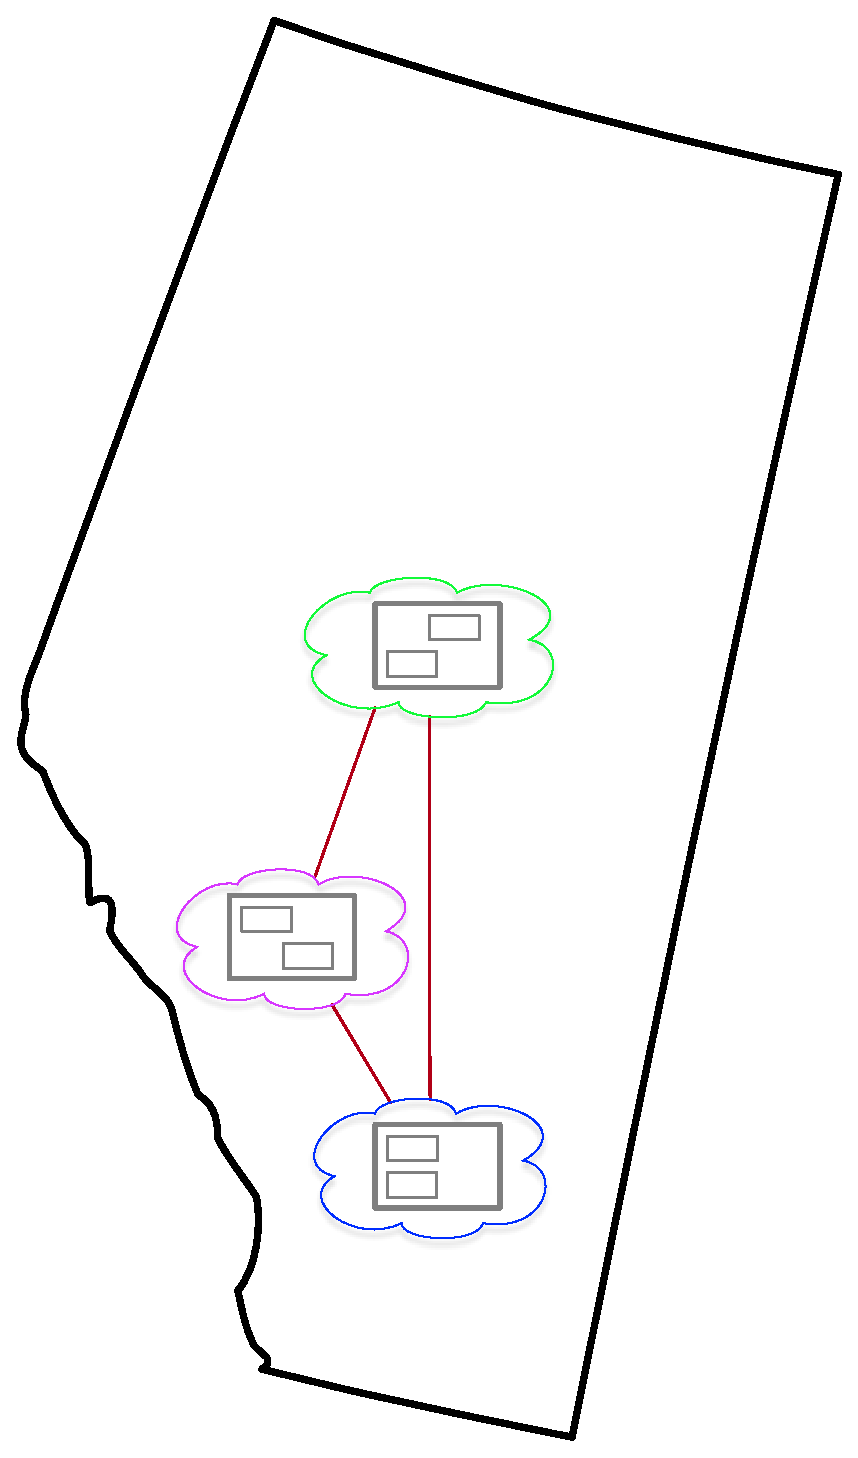
\includegraphics[width=0.75\textwidth]{figures/AB_distributed_table.eps}
\end{column}
\end{columns}

\vskip0.75em

It is up to the database administrator to evaluate the trade-offs between responsiveness and data consistency.
\end{frame}


%
%--------------------------------------------------------------------------------------------------------------
%

\begin{frame}{Moral of the story?}

If an application cannot tolerate inconsistent data (e.g., a banking application), then it will use the 2PC protocol and require all locks to be available before writing.

Most distributed applications (e.g., social networks) can tolerate inconsistent data. The worst that can happen is that users connected to different nodes (e.g., opposite coasts of Canada) of the system don't see each others posts for some time.

\end{frame}










\section{Key/Value Stores}
%!TEX root = lec08_nosql.tex

%
% ------------------------------------------------------------------------------------------------------------
%

\begin{frame}{Key/Value Stores}

Key/Value stores have become popular recently. Example systems include Apache HBASE, Amazon's DynamoDB and Google's BigTable.

\vskip1em

\begin{center}
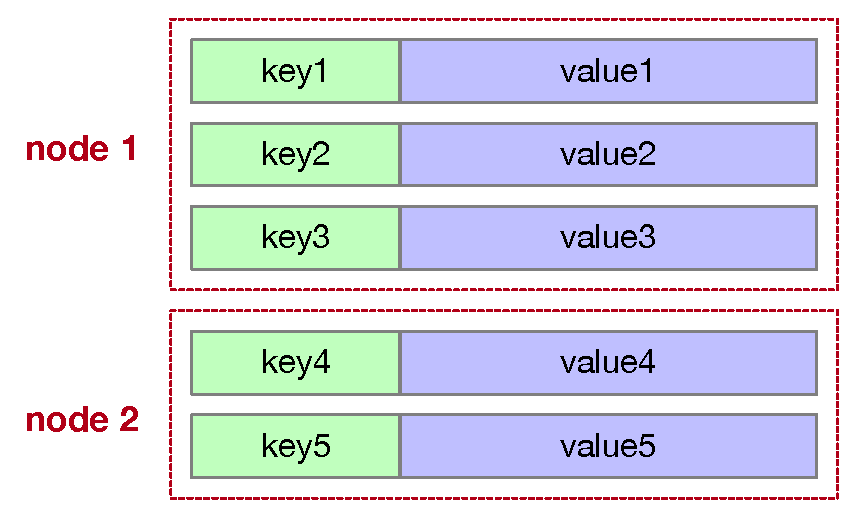
\includegraphics[width=0.5\textwidth]{figures/key_value_store.eps}
\end{center}

\vskip1em

Fundamentally, these systems implement \alert{partitioned tables} as discussed before with the added restriction that \alert{the partition is defined on a singleton key attribute}.
\end{frame}


%
% ------------------------------------------------------------------------------------------------------------
%

\begin{frame}{Why are Key/Value Stores So Popular?}

Except for the keys, each tuple can have its own ``schema'', with its own columns. Also, the ``columns'' can store non-1NF data, like arrays and lists or other data structures.

In other words, these key/value stores are good for storing \textbf{semistructured data}!

\vskip1em
Example:

\begin{center}
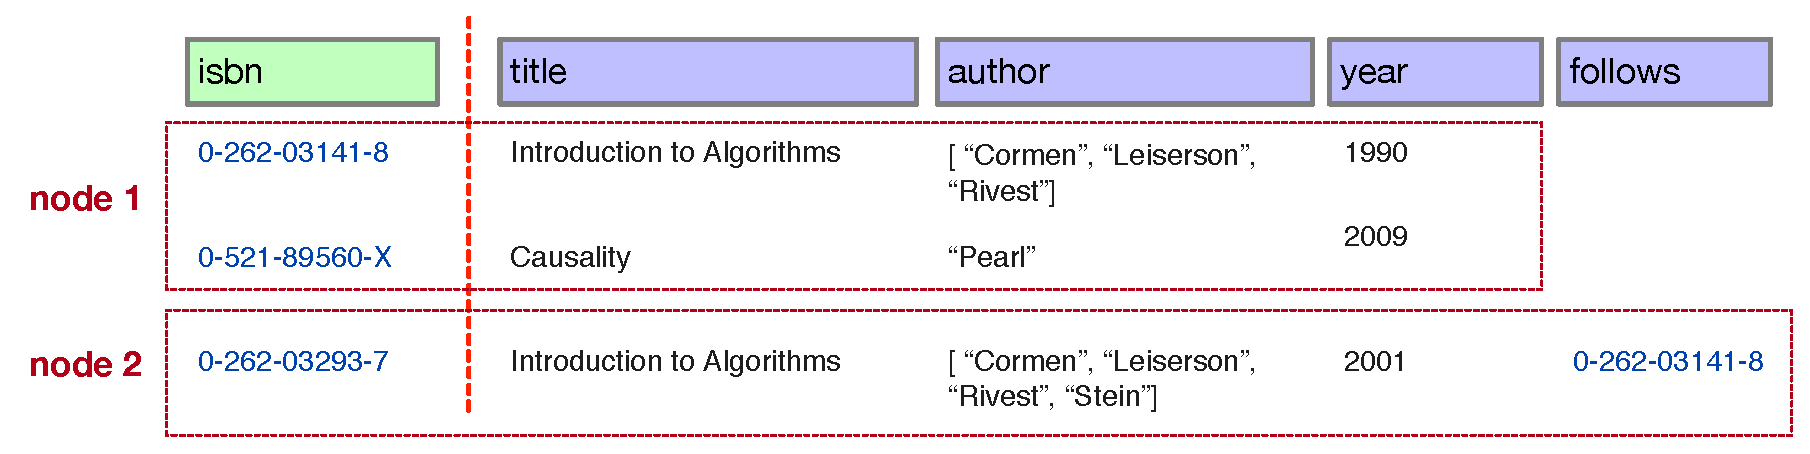
\includegraphics[width=1\textwidth]{figures/key_value_store_example.eps}
\end{center}
\end{frame}

%
% ------------------------------------------------------------------------------------------------------------
%

\begin{frame}

\begin{center}
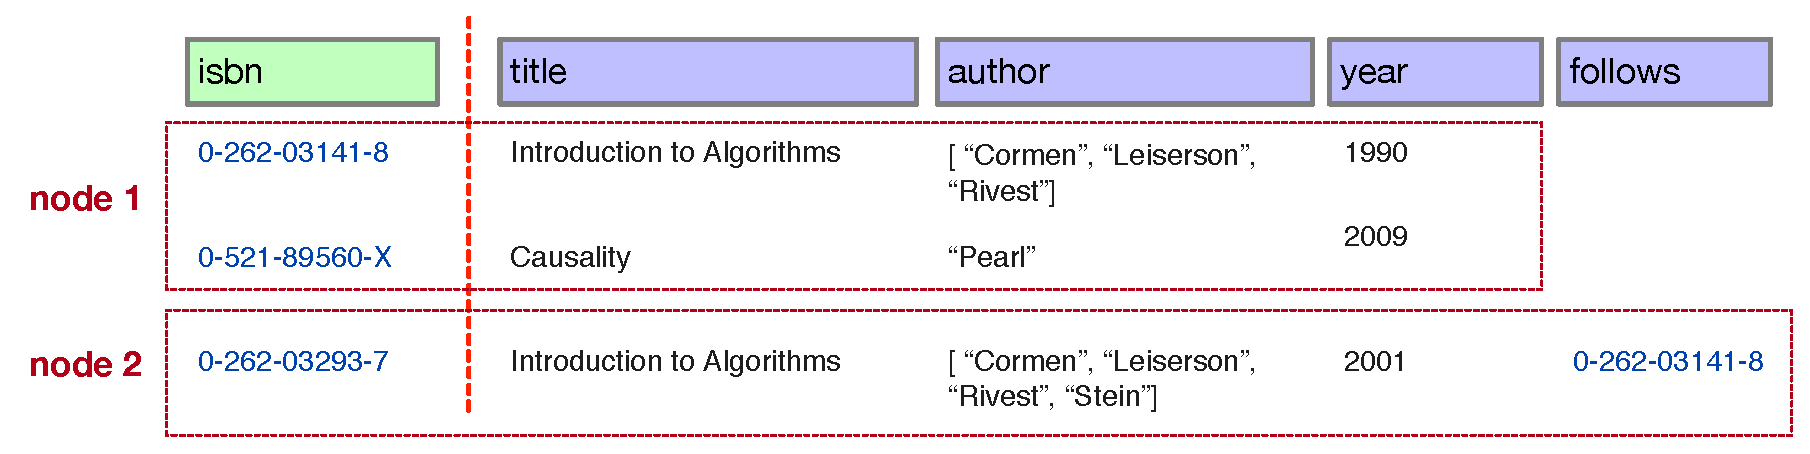
\includegraphics[width=1\textwidth]{figures/key_value_store_example.eps}
\end{center}

\vskip1em

\alert{\textbf{Support for application-level constraints}}?
\begin{itemize}[-,topsep=-5pt]
\item ex: every ISBN in a ``follows'' attribute must match an ISBN of some other ``row'' in the table.
\end{itemize}
 
\vskip1em

The programmer is on their own here... in general, key/value stores \textbf{do not support} constraints like foreign keys. In fact, they don't even support triggers easily.
\end{frame}


%
% ------------------------------------------------------------------------------------------------------------
%

\begin{frame}

Many ``document stores'' are just key-value stores under the hood, where the \textbf{\alert{keys are system-generated}} at insertion time.

These systems allow programs to \textcolor{blue}{C}reate, \textcolor{blue}{R}ead, \textcolor{blue}{U}pdate, or \textcolor{blue}{D}elete objects (\textcolor{blue}{CRUD}).

\vskip2em

\begin{columns}[onlytextwidth]
\begin{column}{0.75\textwidth}
Systems like Elasticsearch also automatically populate indexes as documents are loaded to the ``table''. For example, Elasticsearch indexes allow it to very quickly find documents that match phrases or keywords provided by the user or an application, even for very large collections.
\end{column}
\qquad\begin{column}{0.25\textwidth}

\includegraphics[width=1\textwidth]{figures/elastic.png}
\end{column}
\end{columns}

\vskip1em

CMPUT361 covers those kinds of indexes and a lot more about document processing.
\end{frame}

%
% ------------------------------------------------------------------------------------------------------------
%

\begin{frame}[fragile]

\vskip1em

Example: storing document into an Elasticsearch ``table'' \lstinline!books!:

\vskip1em

\bgroup
\lstset{basicstyle=\ttfamily\scriptsize}

\begin{lstlisting}
POST books/_doc/
{
    "isbn" : "0-262-03141-8",
    "title" : "Introduction to Algorithms",
    "year" : 1990, 
    "authors" :  [ "Cormen", "Leiserson", "Rivest"]
}
\end{lstlisting}
 
Sample output:

\begin{lstlisting}
{
    "_shards" : { "total" : 2, "failed" : 0, "successful" : 2 },
    "_index" : "books",
    "_type" : "_doc",
    -:"_id" : "W0tpsmIBdwcYyG50zbta":-,
    "_version" : 1,
    "_seq_no" : 0,
    "_primary_term" : 1,
    "result": "created"
}\end{lstlisting}

\egroup
\end{frame}

%
% ------------------------------------------------------------------------------------------------------------
%

\begin{frame}{Consistent Hashing}

Consistent hashing is a key ingredient in distributed key/value stores that allows for load balancing even when nodes join or leave the system.

\vskip1em

\begin{columns}[onlytextwidth]
\begin{column}{0.6\textwidth}
Nodes (A, B, C, and D) and objects (1, 2, 3, ...) are hashed to the same circular space (e.g., 32bit hash values with wraparound).

\vskip1em

Objects are assigned to the \textbf{closest} available node in the system.
\end{column}
\begin{column}{0.35\textwidth}
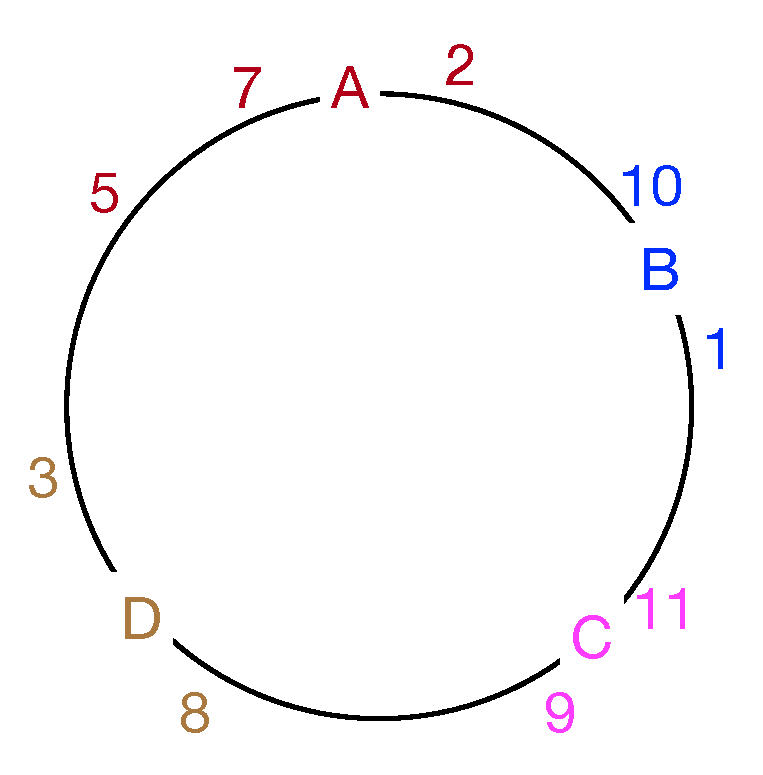
\includegraphics[width=\textwidth]{figures/consistent_hashing_1.eps}
\end{column}
\end{columns}

\end{frame}


%
% ------------------------------------------------------------------------------------------------------------
%

\begin{frame}
\vskip1em

\begin{columns}[onlytextwidth]
\begin{column}{0.6\textwidth}
When a new node joins the cluster, it broadcasts its hash value to other nodes, who respond with a list of documents that are closest to the newcomer.

\vskip1em

Ex: D will take on documents 3 and 5.
\end{column}
\begin{column}{0.35\textwidth}
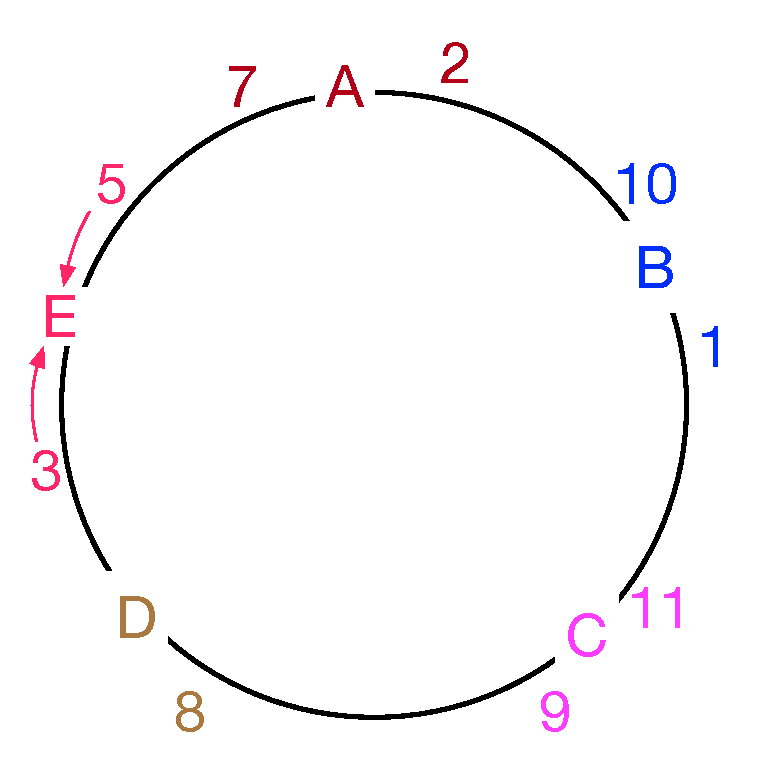
\includegraphics[width=\textwidth]{figures/consistent_hashing_2.eps}
\end{column}
\end{columns}

Documents migrate over time. 

If a request for a document that has not migrated yet arrives, the new node can relay that to the old node that still has the data.

\end{frame}


%
% ------------------------------------------------------------------------------------------------------------
%

\begin{frame}
\vskip1em

\begin{columns}[onlytextwidth]
\begin{column}{0.6\textwidth}
When a node announces it intends to leave the cluster, it sends lists of documents that are to be migrated to its closest neighbors.

\vskip1em

Again, documents migrate gracefully and over time.
\end{column}
\begin{column}{0.35\textwidth}
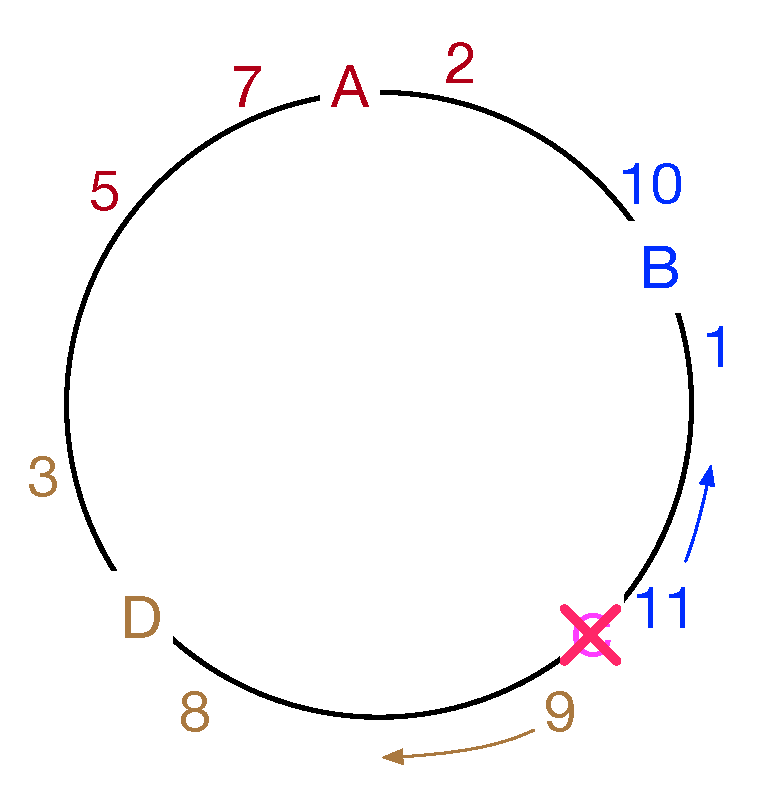
\includegraphics[width=\textwidth]{figures/consistent_hashing_3.eps}
\end{column}
\end{columns}

If a node fails, its neighbors consult all replicas of that node, to take over the documents that are now (temporarily) unavailable.

\end{frame}

\section{Distributed File Systems and Map/Reduce}
%!TEX root = lec08_nosql.tex

\lstset{
    style=cmput391,
	emph=[3]{map,reduce,includes,keys,values,emit},
	emphstyle=[3]\ttfamily\bfseries\color{accent},
	emph=[4]{function,if,else,return,for,in,var},
	emphstyle=[4]\ttfamily\bfseries\color{blue}
}


\def\myblue#1{\textcolor{blue}{#1}\xspace}
\def\myred#1{\textcolor{red}{#1}\xspace}

%
% ----------------------------------------------------------------------------------------------------
%


\begin{frame}{Data Processing with Map/Reduce}

\begin{center}
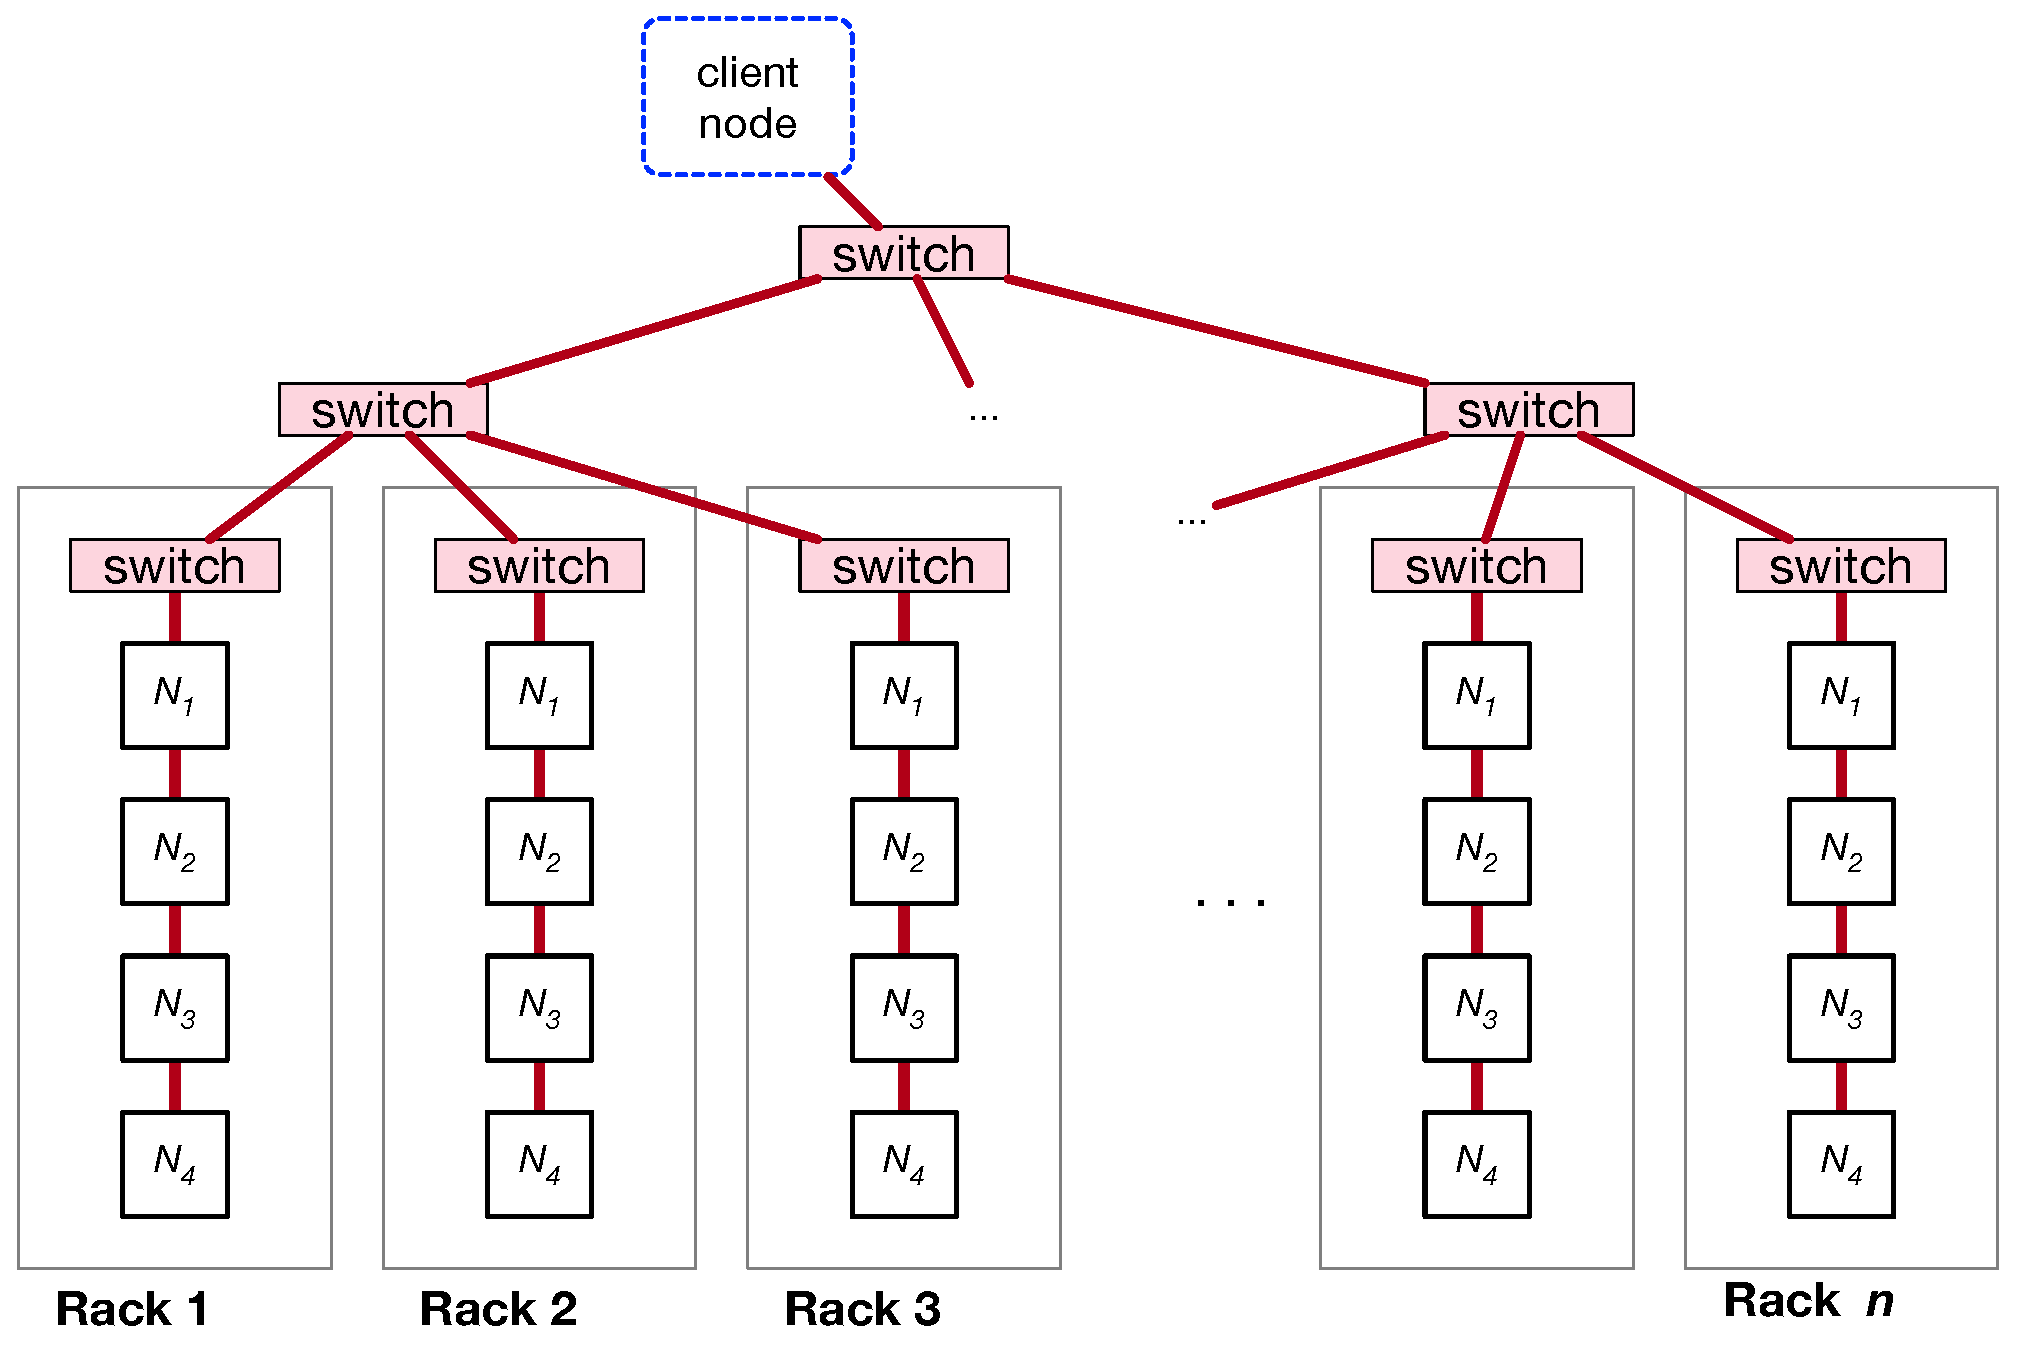
\includegraphics[width=0.75\textwidth]{figures/map_reduce_racks.eps}
\end{center}

We now look into using a shared-nothing cluster as a parallel computer for data processing.
\end{frame}

%
% ----------------------------------------------------------------------------------------------------
%


\begin{frame}

Map/Reduce is a functional programming paradigm that can be easily parallelized.

Very popular inside Google from 2004:
{\footnotesize\url{https://research.google.com/archive/mapreduce-osdi04-slides/index.html}}

Facebook and Yahoo both invested in the open source Apache Hadoop project\\
{\footnotesize{\url{https://wiki.apache.org/hadoop/PoweredBy\#F}}}\\
{\footnotesize{\url{https://wiki.apache.org/hadoop/PoweredBy\#Y}}}\\

\end{frame}


%
% ----------------------------------------------------------------------------------------------------
%


\begin{frame}{HDFS: Redundancy and Load Balancing}

Each blocks of a file is replicated (usually twice) across nodes and across racks (to account for network component failures).

The ``directory'' is kept by a ``name node'' (in Hadoop terminology), which tells the client which nodes have the data.

Any node with the data can process it.

\begin{center}
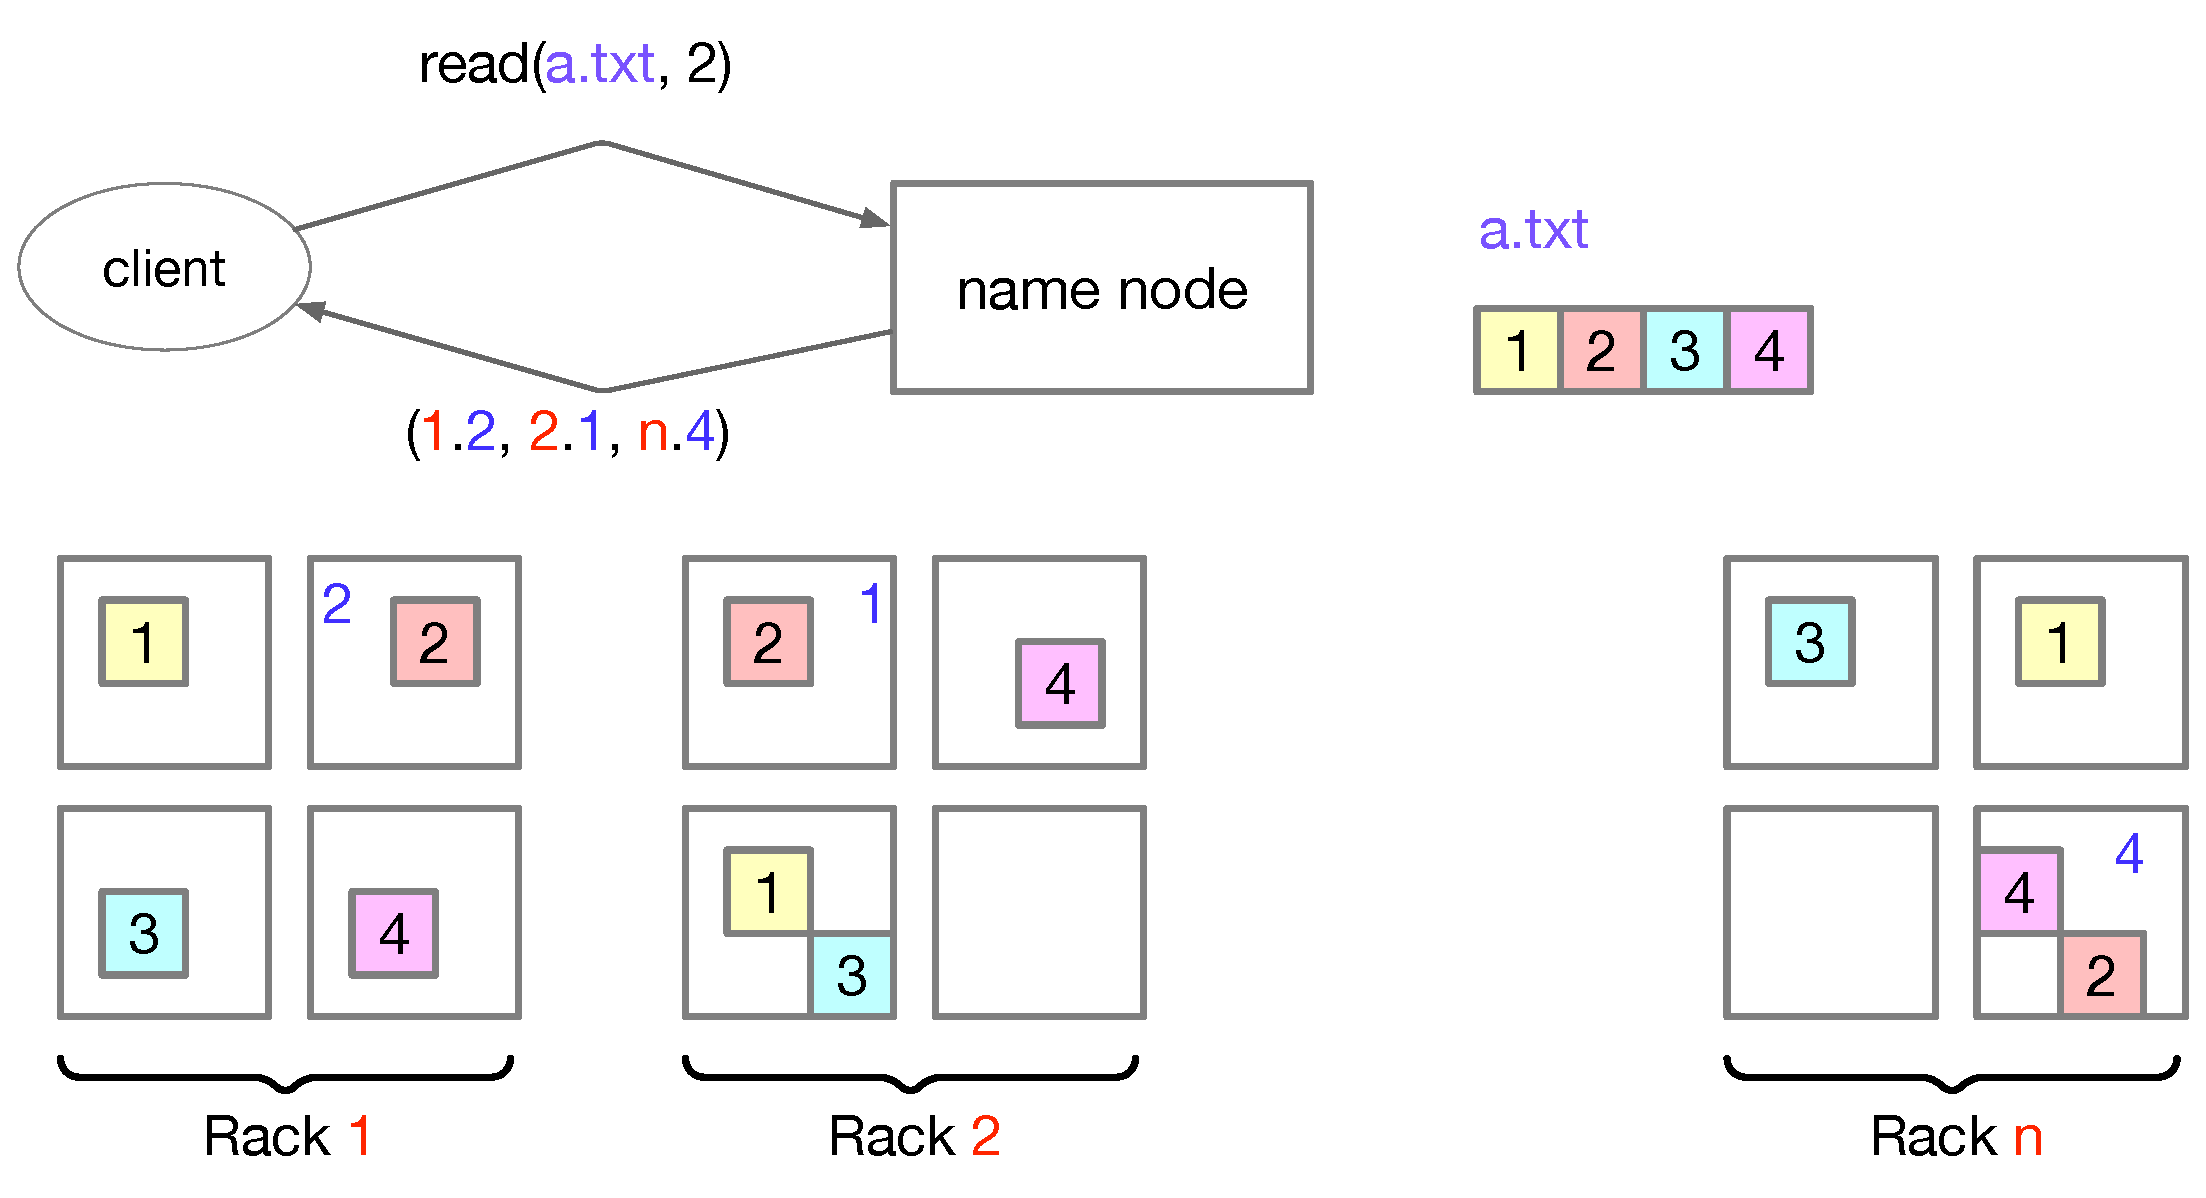
\includegraphics[width=0.75\textwidth]{figures/hdfs_blocks.eps}
\end{center}

\end{frame}

%
% ----------------------------------------------------------------------------------------------------
%


\begin{frame}{Programming Parallel Computers is Hard}

\blue{\textbf{Challenge \#1}}: it is hard to design the control flow when multiple computations happen \emph{at the same time} and in different computing nodes...
\begin{itemize}[-]
\item It is \textbf{very hard} to debug such designs.
\end{itemize}

\blue{\textbf{Challenge \#2}}: giving the programmers a  \alert{programming paradigm} simple enough so that we can easily express computations, yet \textbf{powerful enough} to be practical.

\vskip1em

\begin{block}{}
\alert{MapReduce} is a simple functional and powerful programming paradigm. Computations in MapRedure are:
\begin{itemize}[-,noitemsep]
\item easy to understand by humans
\item can be executed in parallel in massive clusters
\end{itemize}
\end{block}

\end{frame}

%
% ----------------------------------------------------------------------------------------------------
%


\begin{frame}{Data locality is important}

The goal of using a cluster was to avoid the communication cost of moving all the data around.
\begin{itemize}[-]
\item Some communication is unavoidable, however.
\end{itemize}

Parallel programs often alternate between:
\begin{itemize}[-,noitemsep]
\item Computing with \emph{local data} (no communication).
\item Exchanging results of local computation with other nodes.
\end{itemize}


\blue{\textbf{Challenge \#3}}: avoiding ``all-to-all'' communication model where every node exchanges data with every other node

\begin{block}{}
\alert{MapReduce computations work in stages}: map operations work on local data, reduce operations aggregate results. Communications are directed.
\end{block}
\end{frame}

%
% ----------------------------------------------------------------------------------------------------
%


\begin{frame}

\vskip2em

\begin{block}{Stages of MapReduce computations}
\begin{itemize}[-,noitemsep]
\item map operations work on local data, and produce \alert{$\textit{key},\textit{value}$} tuples
\item tuples are grouped together by key
\item all tuples with \alert{the same key} are sent to the same reduce task
\end{itemize}
\end{block}

\vskip1em 

\begin{center}
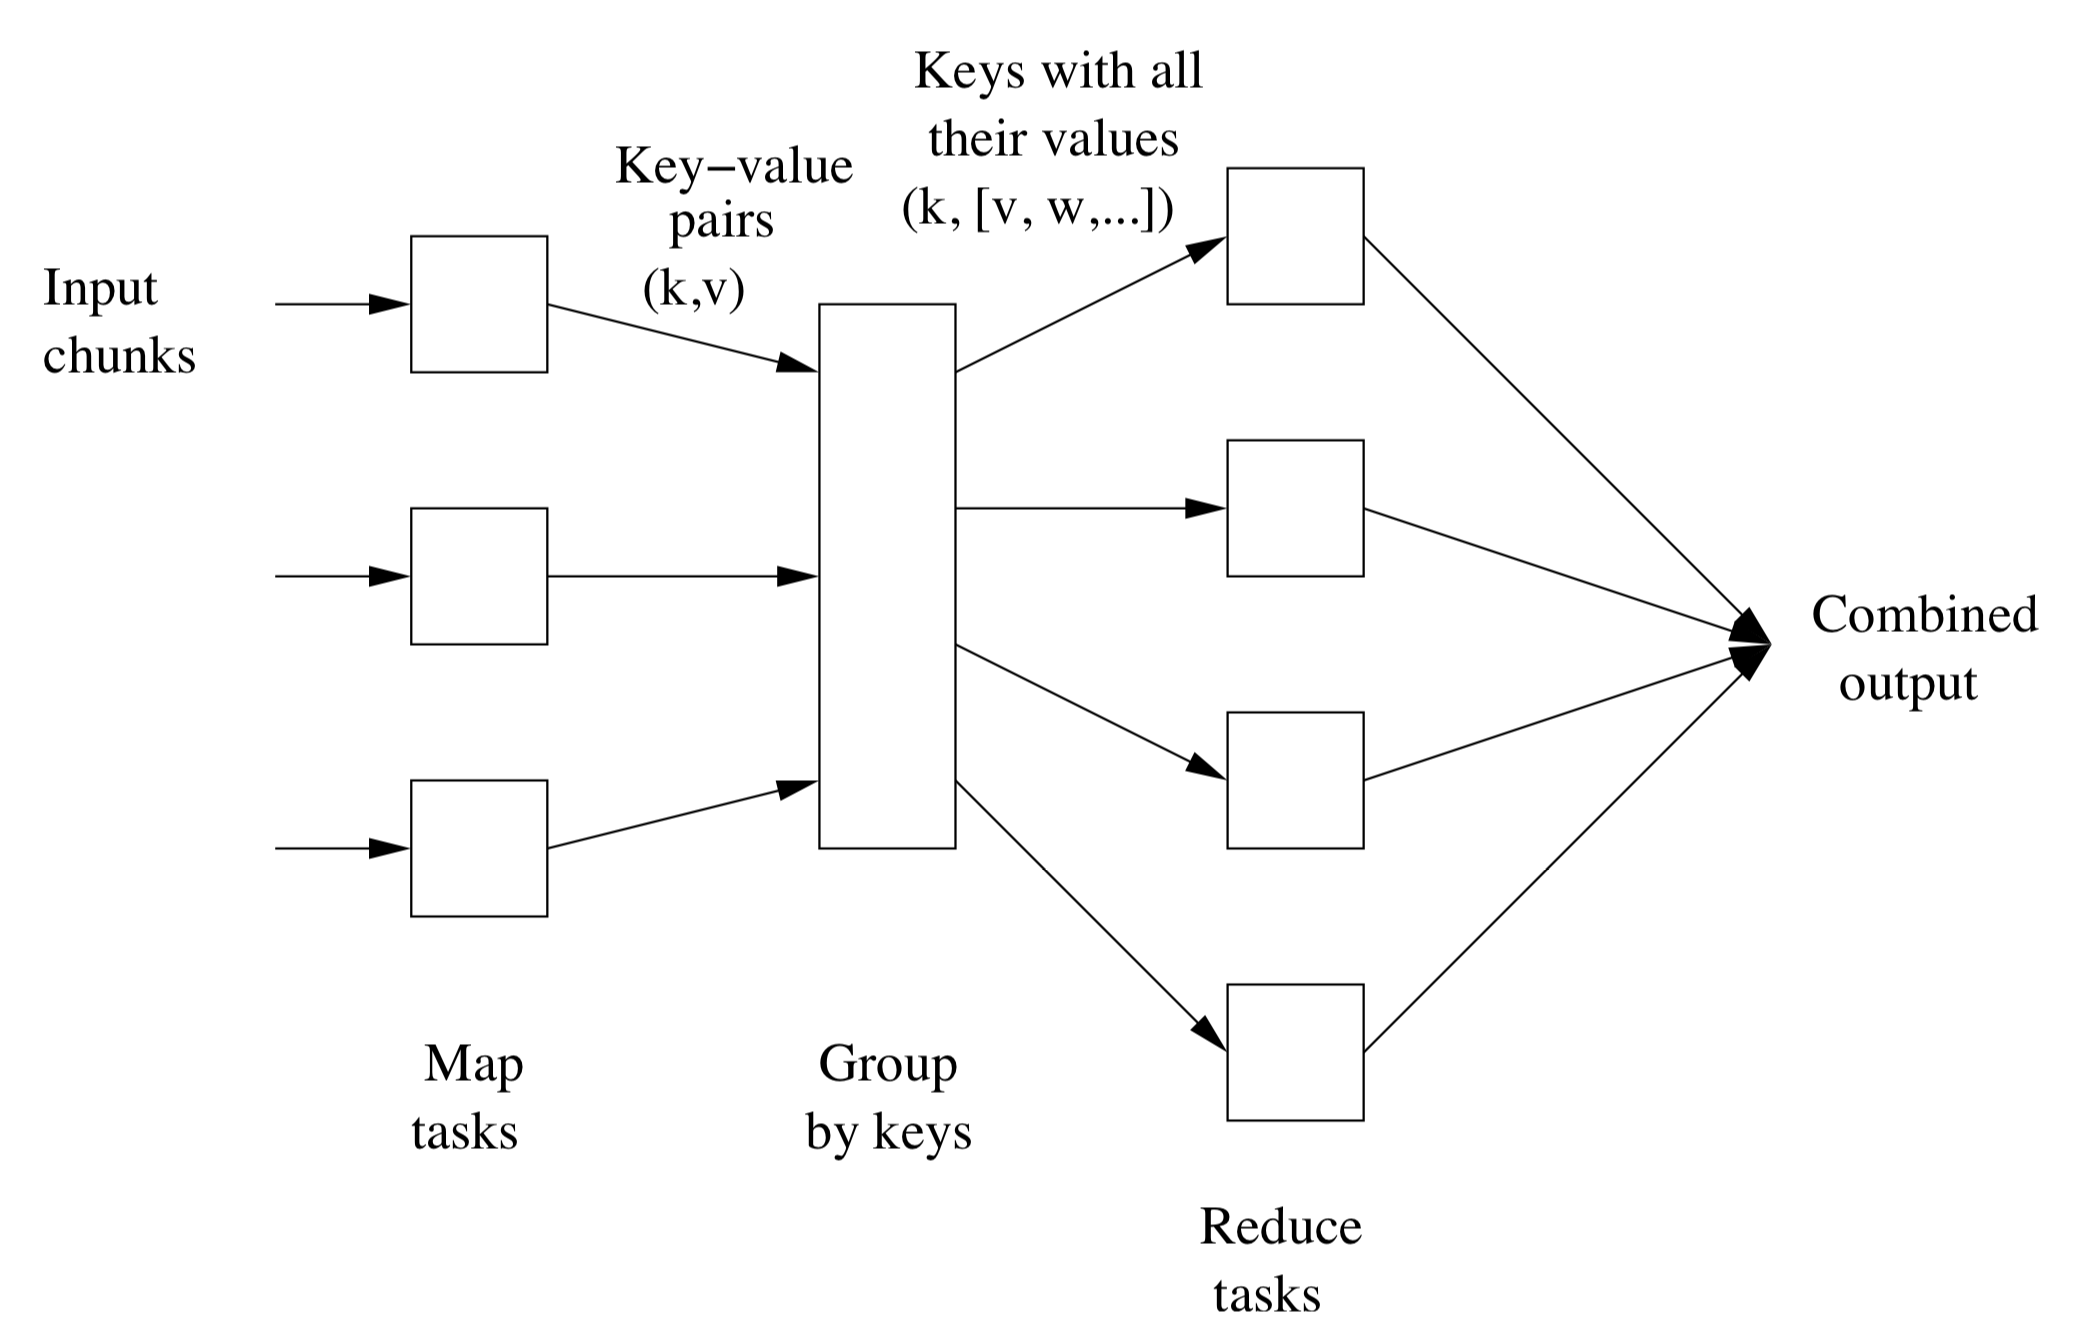
\includegraphics[width=0.75\textwidth]{figures/mapreduce_workflow.png}
\end{center}
\end{frame}


%
% ----------------------------------------------------------------------------------------------------
%

\begin{frame}{Execution of a MapReduce job}
\begin{center}
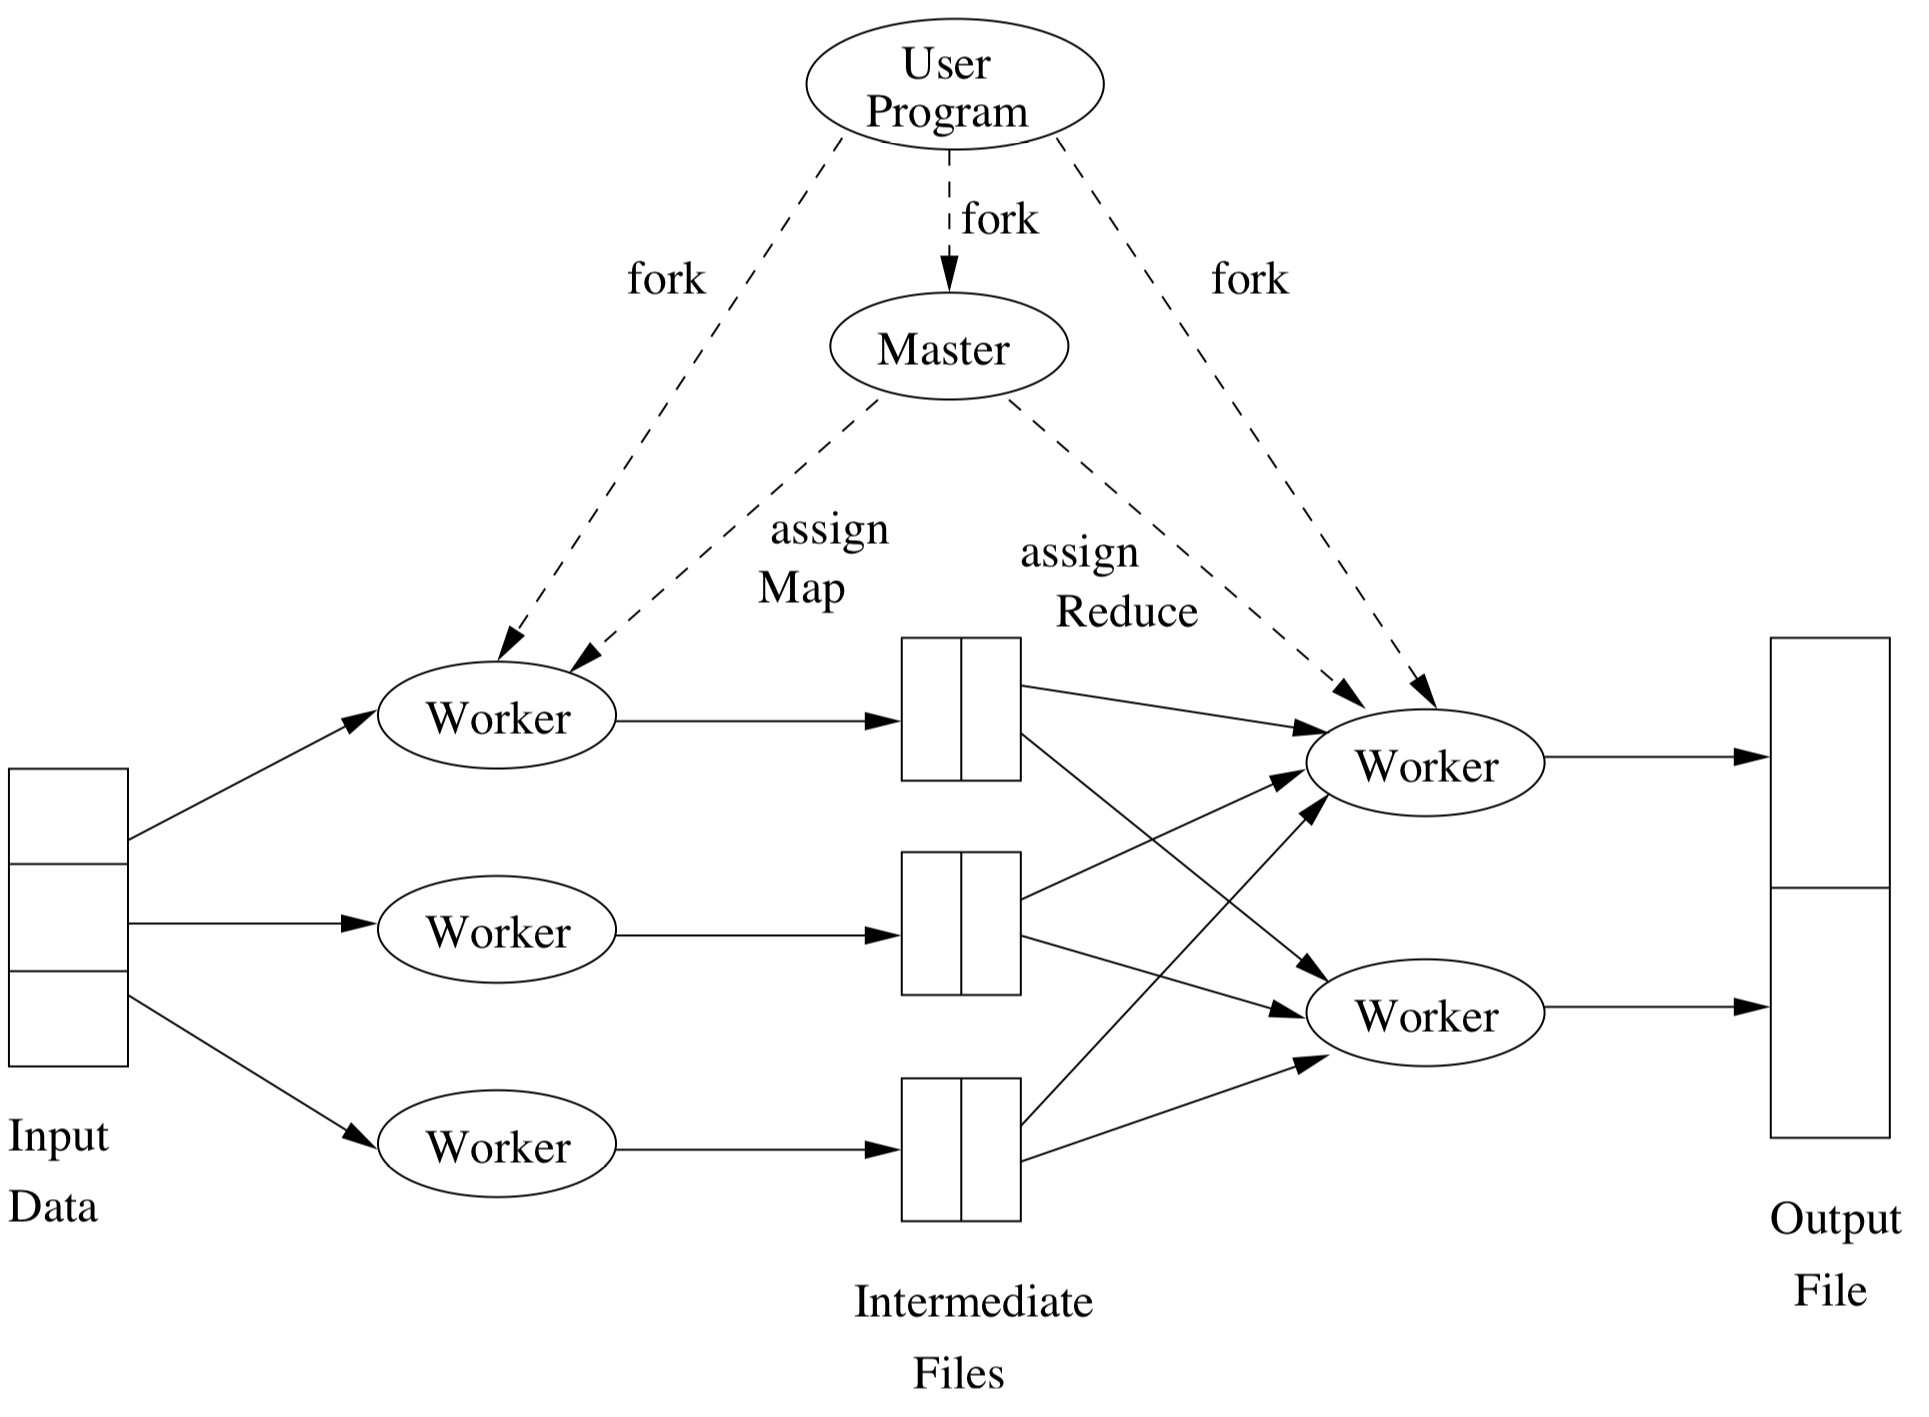
\includegraphics[width=0.65\textwidth]{figures/mapreduce_forking.png}
\end{center}

\vspace*{-1em}

The program specifies the \lstinline{map()} and \lstinline{reduce()} functions 

The \myblue{Master} process starts ``worker'' processes to complete all \lstinline{map()} tasks; once they are done, the \myblue{Master} starts ``workers'' for the \lstinline{reduce()} tasks.

\end{frame}


%
% ----------------------------------------------------------------------------------------------------
%


\begin{frame}[fragile]{Word count with MapReduce}

Suppose we want to \alert{count the number of times each word appears} in a large corpus of texts (e.g., millions of documents).
\begin{itemize}[-,noitemsep]
\item Each compute node has many documents in its local storage
\item No compute node has all occurrences of any single word
\end{itemize}

\vskip2em

General idea:
\begin{enumerate}[(1),noitemsep]
\item \alert{Map}: emit tuples \myblue{$(w,1)$} for every occurrence of a word in a document
\item \alert{Group} all streams of tuples with the same word
\item \alert{Reduce}: return tuple \myblue{$(w, l)$} where \myblue{$l$} is the number of tuples for word \myblue{$w$}
\end{enumerate}

\end{frame}

%
% ----------------------------------------------------------------------------------------------------
%


\begin{frame}[fragile]

\begin{block}{Map operation}
For every file \myred{\emph{f}} stored locally, do:
\begin{itemize}[-]
\item normalize and tokenize \myred{\emph{f}} into a list of words \lstinline[mathescape]![w$_1$, w$_2$, $\ldots$, w$_n$]!
\item for every word \myred{\emph{w}} in \lstinline[mathescape]![ w$_1$, w$_2$, $\ldots$, w$_n$]!
\begin{itemize}[$\rightarrow$]
\item \alert{emit} tuple \lstinline[mathescape]!(w, 1)!
\end{itemize}
\end{itemize}
\end{block}

\vskip1em

\begin{block}{Reduce operation}
\textbf{Input}: stream of tuples $t_1=(w_j, 1), t_2=(w_j,1),\ldots, t_k=(w_j,1)$\\
\textbf{Output}: \alert{$k$}
\end{block}

\vskip1em

Where does the output go?

The reduce operation can write data to a file. So, each compute node could open a file for each word it received...
\end{frame}


%
% ----------------------------------------------------------------------------------------------------
%


\begin{frame}{Execution of a MapReduce job}
\begin{center}
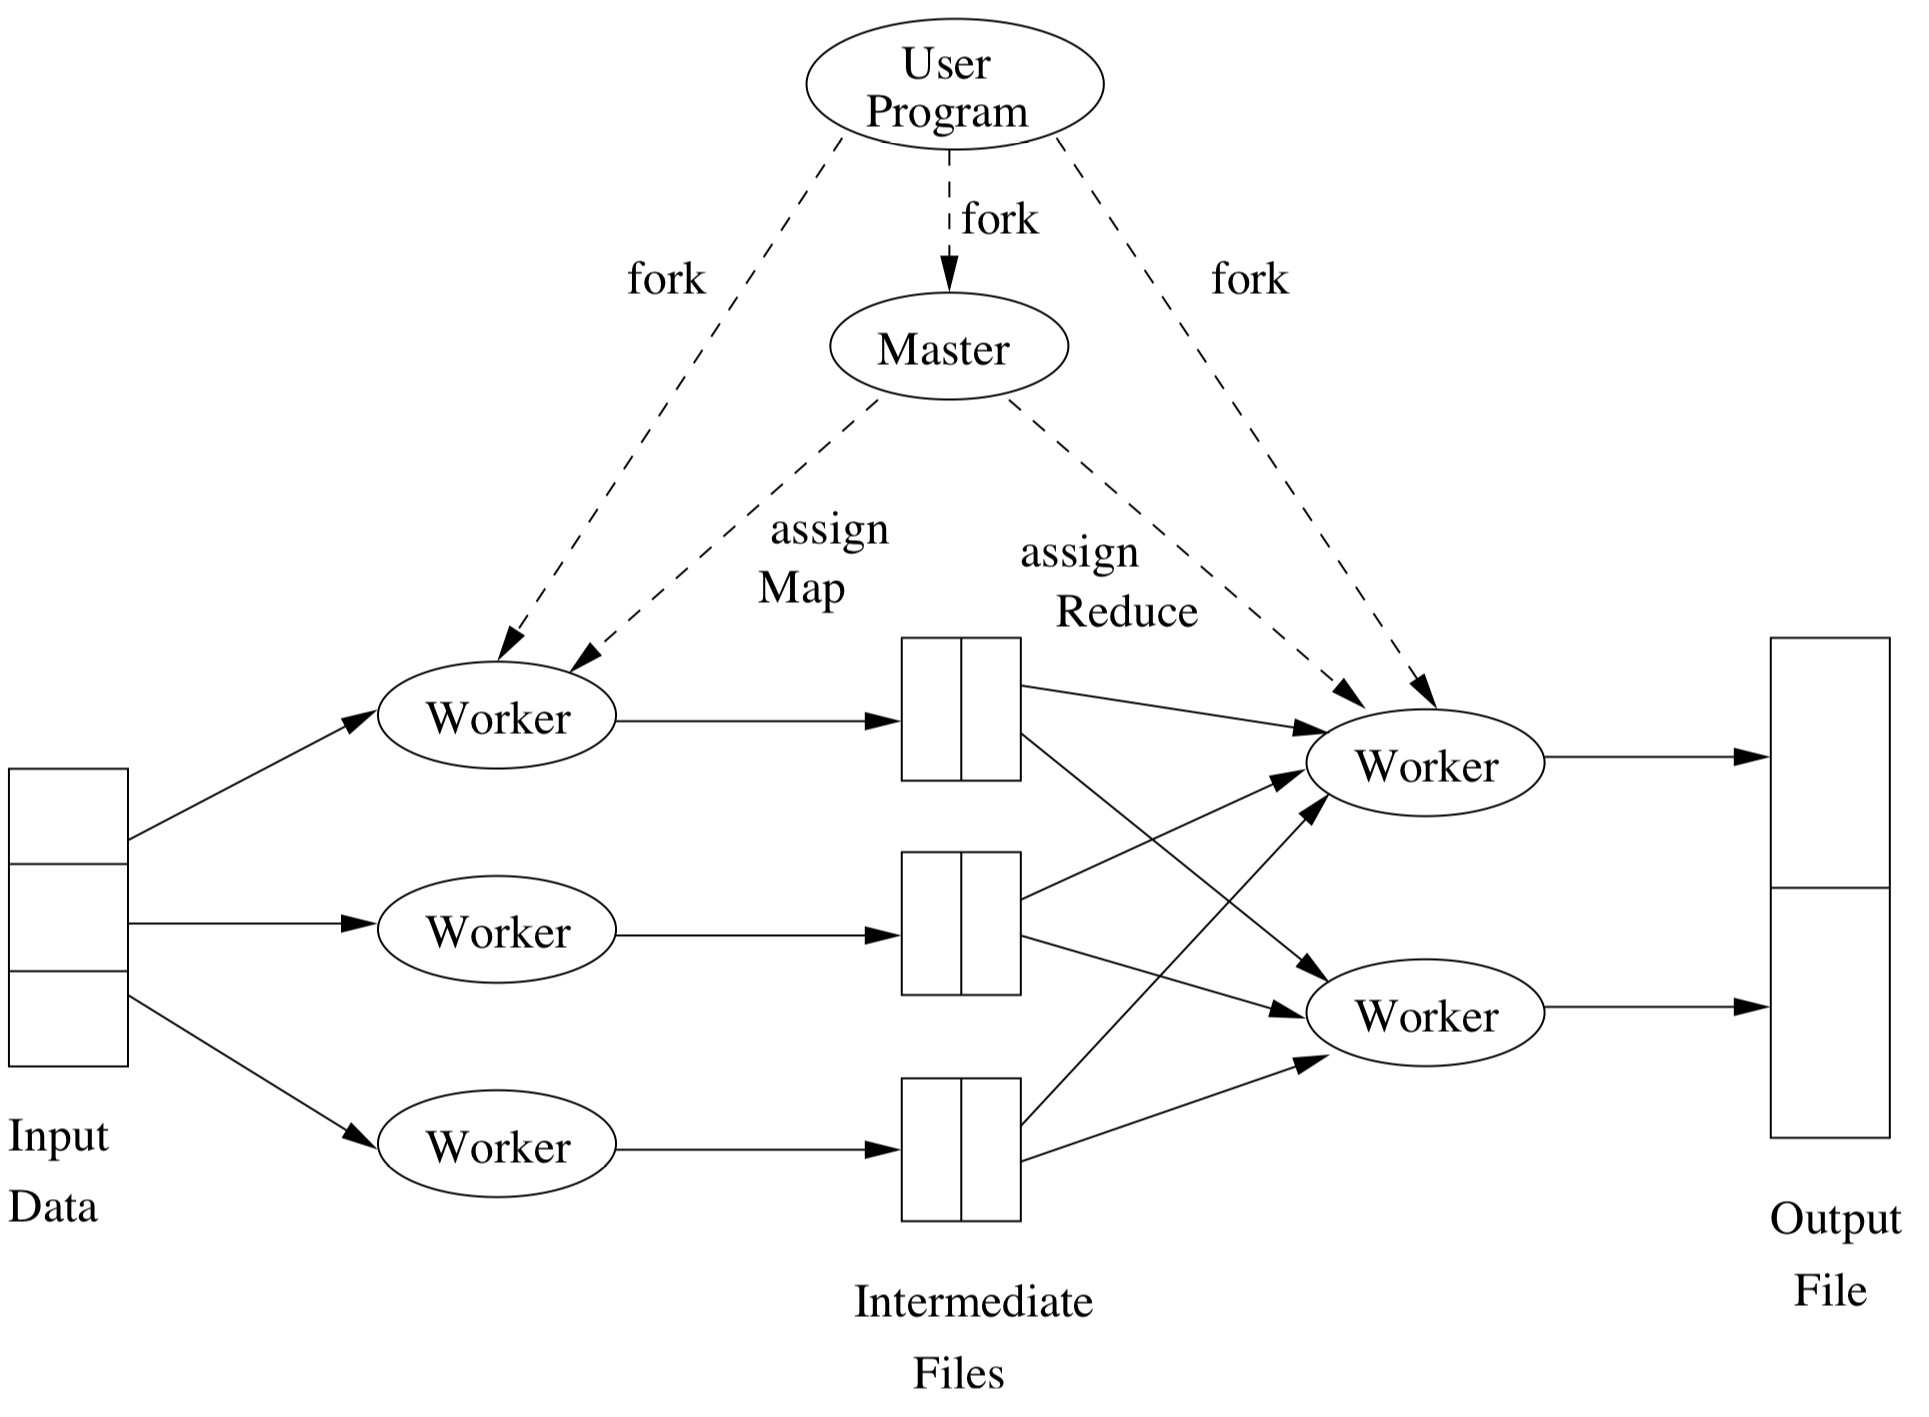
\includegraphics[width=0.65\textwidth]{figures/mapreduce_forking.png}
\end{center}

\vspace*{-1em}

The program specifies the \lstinline{map()} and \lstinline{reduce()} functions 

The \myblue{Master} process starts ``worker'' processes to complete all \lstinline{map()} tasks; once they are done, the \myblue{Master} starts ``workers'' for the \lstinline{reduce()} tasks.

\end{frame}


%
% ----------------------------------------------------------------------------------------------------
%


\begin{frame}
\centering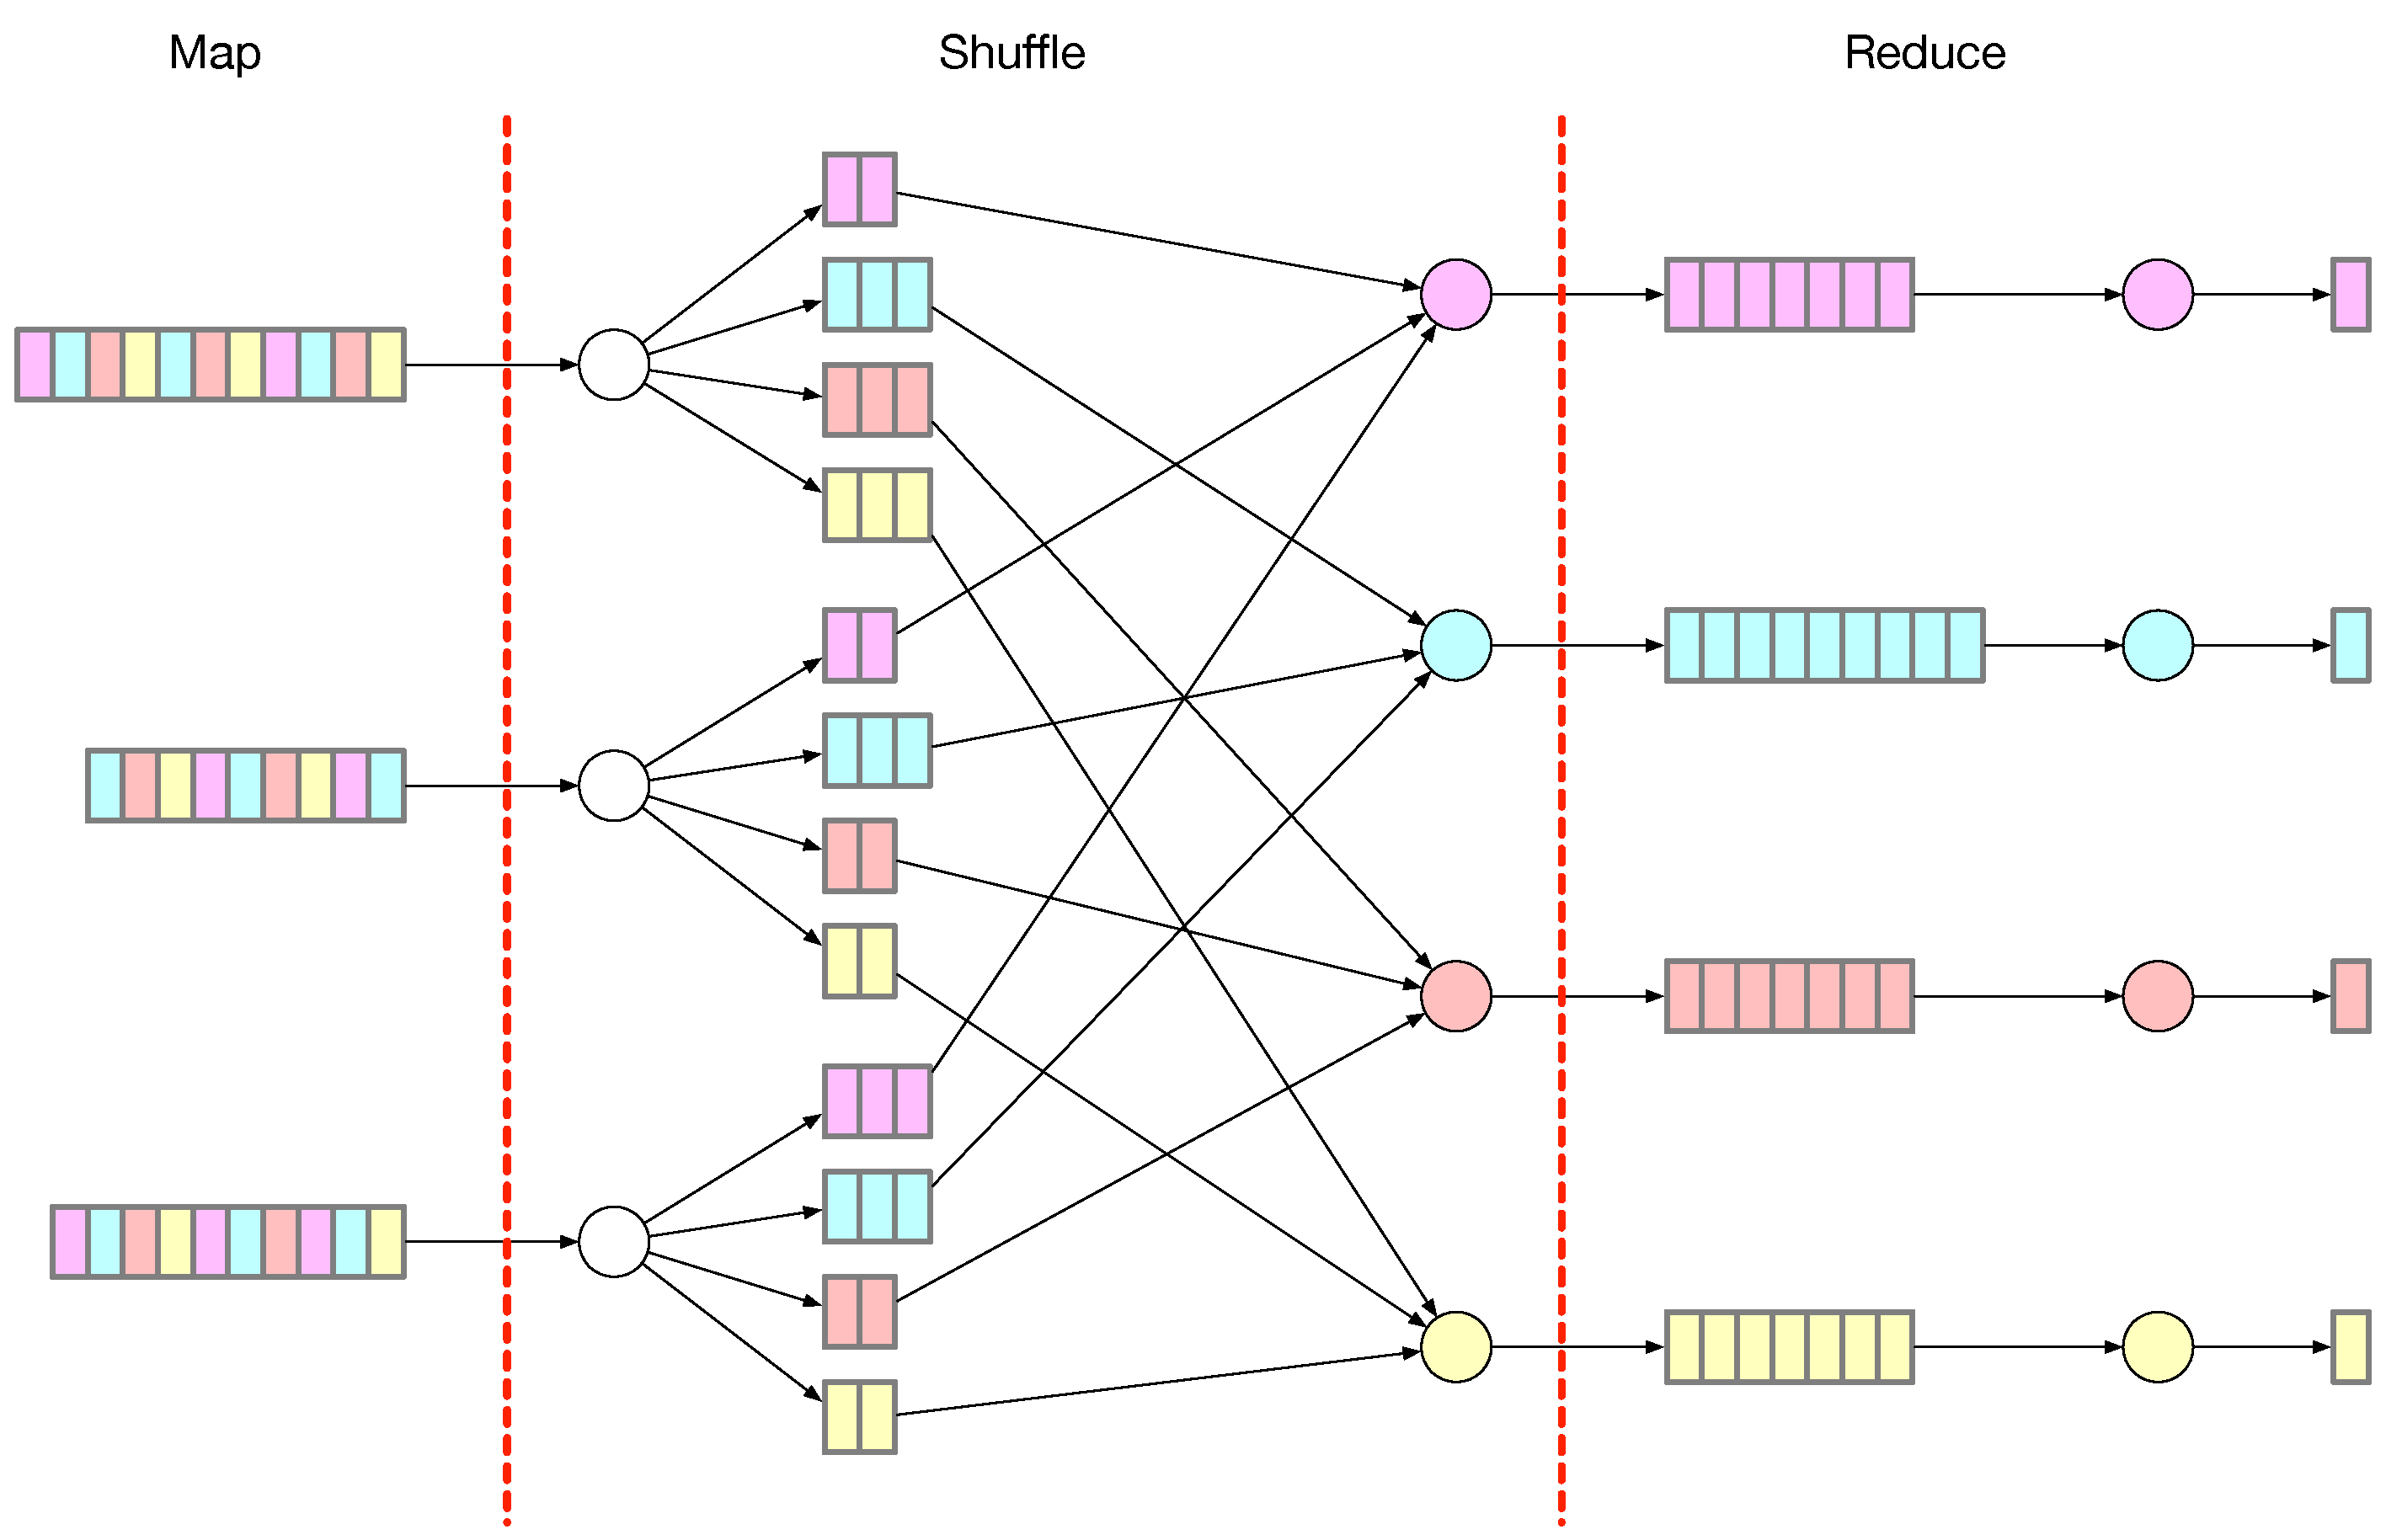
\includegraphics[width=\textwidth]{figures/map_reduce_shuffle.eps}
\end{frame}


%
% ----------------------------------------------------------------------------------------------------
%


\begin{frame}{Networking Cost}

\begin{center}
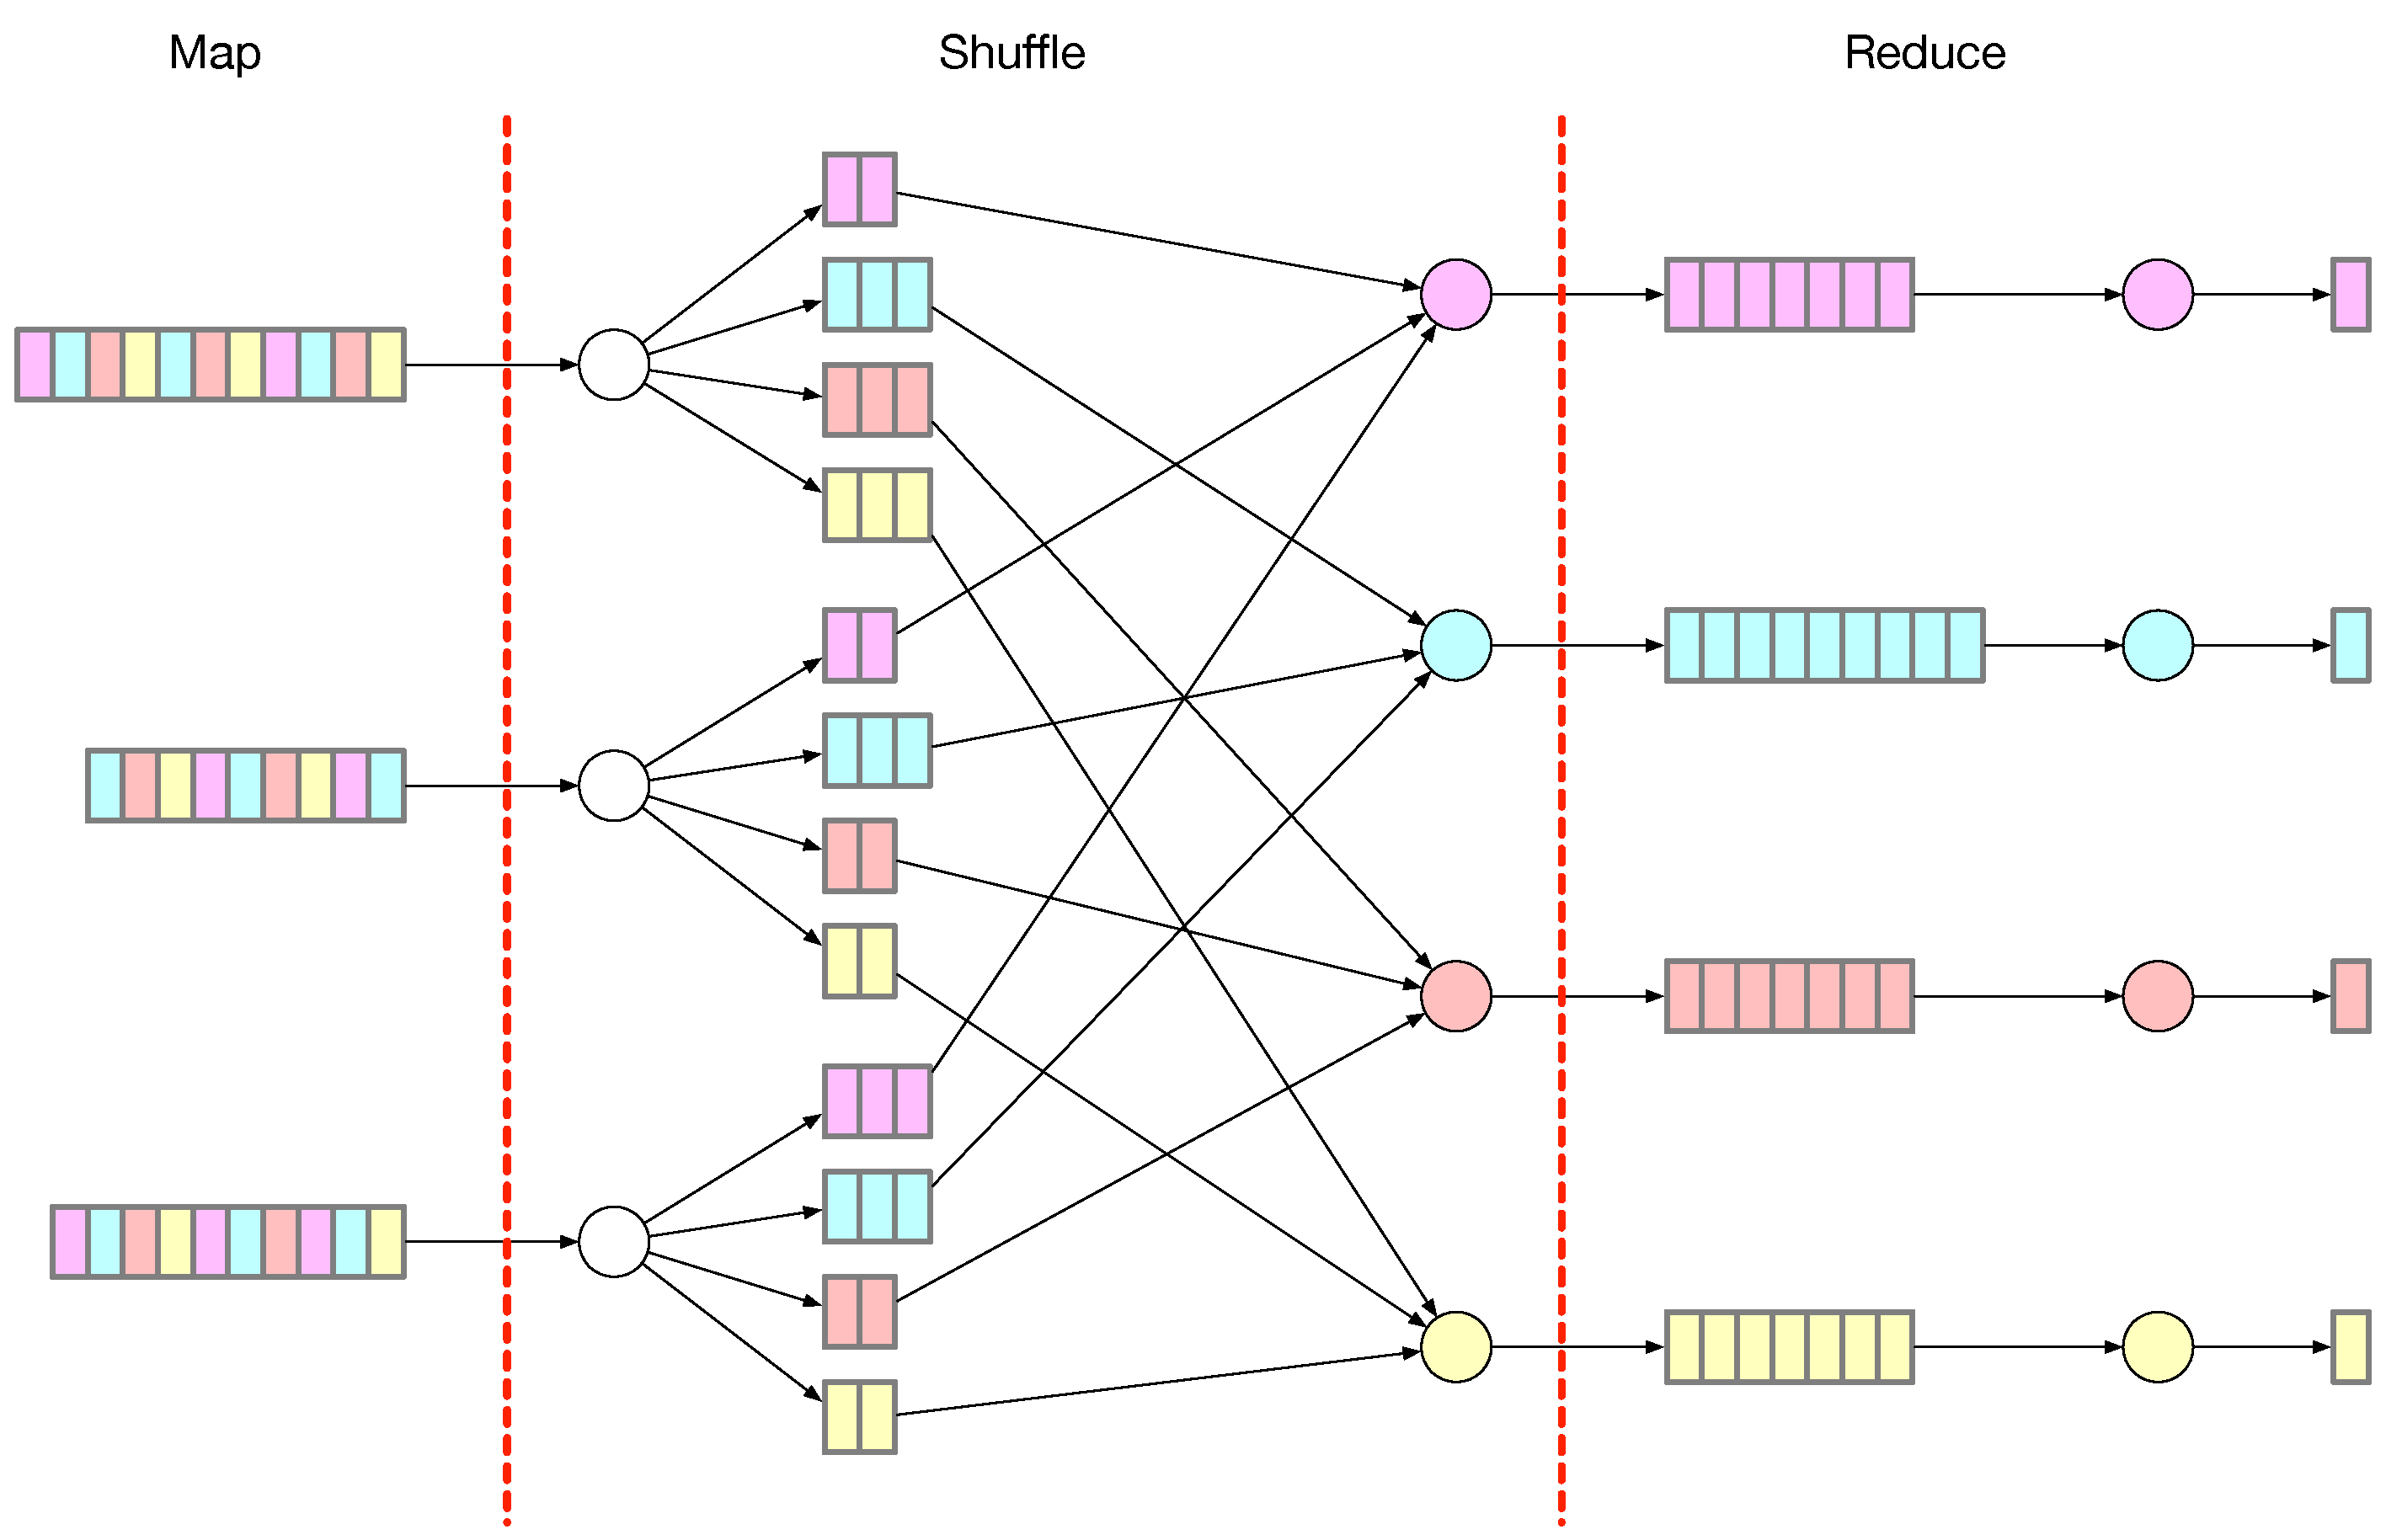
\includegraphics[width=0.5\textwidth]{figures/map_reduce_shuffle.eps}
\end{center}

The master assigns keys to nodes, deciding which nodes will perform which \lstinline{reduce()} operations.

Then, the nodes ``shuffle'' the stream of tuples, sending each tuple to the right \lstinline{reduce()} node.

\alert{\textbf{NOTE THAT} each node keeps at least one list of tuples though!}
\end{frame}


%
% ----------------------------------------------------------------------------------------------------
%


\begin{frame}{Obvious optimization}

The example so far is the ``textbook'' word count, where each tuple has count 1 for every word. 

An obvious optimization would be for the \lstinline!map()! operation to emit \alert{one tuple per word} among all documents it reads. This is possible, of course, only if the computing node has enough RAM to keep that map in memory.

\vskip1em

But even if the node does not have a lot of memory, it can keep accumulating word counts until all RAM is used up. At that point, the node can emit all tuples and start counting again.

\end{frame}

%
% ----------------------------------------------------------------------------------------------------
%


\begin{frame}{Multi-stage computations}

It is possible to have more complex computations involving several MapReduce phases. Below is one example MapReduce computation following finding individual word counts. 

Note that each node is left with a list of tuples, each with the count of an individual word, and that no two nodes have the count of the same word.

\vskip1em

\alert{Finding total number of words:}

\begin{block}{\lstinline{map()}}
Go over all words in the node and \alert{emit} a single tuple (\emph{\myblue{k}},\myred{\emph{total}}) where total is the sum of individual word counts in the node.
\end{block}

\begin{block}{\lstinline{reduce()} -- note that all tuples have the same key \myblue{\emph{k}}}
Sum up the values in the incoming tuples.
\end{block}
\end{frame}


%
% ----------------------------------------------------------------------------------------------------
%


\begin{frame}

\alert{Finding word(s) with highest frequency:}

\begin{block}{\lstinline{map()}}
Go over all word counts in the node; \alert{emit} a single tuple \lstinline[mathescape]!($k$,($c$,(w$_1$, w$_2$, $\ldots$, w$_n$)))! where:
\begin{itemize}[-,noitemsep]
\item $k$ is any constant
\item $c$ is the highest word frequency among all words in the node
\item \lstinline[mathescape]!w$_1$, w$_2$, $\ldots$, w$_n$! are all the words with count $c$
\end{itemize}
\end{block}

\begin{block}{\lstinline{reduce()} -- note that all tuples have the same key \myblue{\emph{k}}}
Go over the stream of tuples; find the highest count; return all words with that count.
\end{block}

Note that the highest count can be found in multiple nodes... so the reducer may have to merge word lists coming from different mappers.
\end{frame}

%
% ----------------------------------------------------------------------------------------------------
%


\begin{frame}{Matrix Operations in Map/Reduce}

Google's PageRank algorithm can be elegantly stated and efficiently computed as a series of matrix multiplications, which they implemented using Map Reduce for scalability reasons.

In fact, Google was probably among the first company to build a fortune on linear algebra.

Let $A$ be a $m\times n$ matrix (e.g., the adjacency matrix of the Web graph), and $\vec{v}$ be an $n$-dimensional vector.

\begin{block}{Vector-matrix product $x_i=\displaystyle\sum_{j=1}^{n}a_{ij}v_j$}
\begin{itemize}[-,noitemsep]
\item \lstinline{map()}: taking the entire $\vec{v}$ as input, compute $a_{ij}v_j$ for all cells of the matrix stored at the node; emit tuple $(i, m_{ij}v_j)$.
\item \lstinline{reduce()}: sum all partial values of $a_{ij}v_j$ for each key $i_x$, and write $i_x$ and the sum to the output.
\end{itemize}
\end{block}
\end{frame}

%
% ----------------------------------------------------------------------------------------------------
%


\begin{frame}

Let $A$ be a $m\times p$ matrix $B$ be an $p\times n$ matrix. 

The \alert{product} $AB$ is the $m \times n$ matrix $C$, in which element $c_{ij} = \displaystyle\sum_{k} a_{ik}b_{kj}$ and 

One way to compute $C$ is through two map/reduce stages:



\begin{block}{Matrix Multiplication Stage 1}
\begin{itemize}[-,noitemsep]
\item \lstinline{map()}: emit each matrix element for whatever matrix data is in the node. That is, emit all $(k,(A, i, a_{ik}))$ and $(k,(B, j, b_{kj}))$.
\item \lstinline{reduce()}: for each pair $(A, i, a_{ik})$ and $(B, j, b_{kj})$ that agree on the same $k$, write the tuple $(k,i,j,a_{ik}b_{kj})$.
\end{itemize}
\end{block}

At the end Stage 1, we can build a separate list for each value of $k$: $(i_1, j_1, v_1), (i_2, j_2, v_2), \ldots, ((i_p, j_p), v_p)$ with all combinations of $i,j$ and factors whose sum that will go into cell $c_{ij}$.
\end{frame}

%
% ----------------------------------------------------------------------------------------------------
%


\begin{frame}

The first stage computes, effectively lists of the form

\[(k, [(i_1, j_1, v_1), (i_2, j_2, v_2), \ldots, ((i_p, j_p), v_p)] \]

In this stage we compute an \emph{aggregate} (the sum) of these lists.

\vskip1em

\begin{block}{Matrix Multiplication Stage 2}
\begin{itemize}[-,noitemsep]
\item \lstinline{map()}: go through the tuples from the previous stage and emit $((i_1,j_1), v_1), ((i_1, j_1), v_2), \ldots ((i_p, j_p), v_p)$.
\item \lstinline{reduce()}: sum up all values with the same $(i,j)$, and write $((i,j) \displaystyle\sum_{p}v_p)$ to the final output.
\end{itemize}
\end{block}
\end{frame}

\def\MRclusterExample{
\draw (0,2) rectangle (1.5,3.5);
\node (n1t1) at (0,3.5) [anchor=north west] {\lstinline!R(1,2)!};
\node (n1t2) [below=0em of n1t1] {\lstinline!R(2,1)!};
\node (n1t3) [below=0em of n1t2] {\lstinline!S(1,2)!};
\node [left=0.0125cm of n1t1] {\small $N_1$};

\draw (0,0) rectangle (1.5,1.5);
\node (n2t1) at (0,1.5) [anchor=north west] {\lstinline!R(4,2)!};
\node (n2t2) [below=0em of n2t1] {\lstinline!R(5,2)!};
\node (n2t3) [below=0em of n2t2] {\lstinline!S(3,2)!};
\node [left=0.0125cm of n2t1] {\small $N_2$};

\draw (2.5,2) rectangle (4,3.5);
\node (n3t1) at (2.5,3.5) [anchor=north west] {\lstinline!R(3,1)!};
\node (n3t2) [below=0em of n3t1] {\lstinline!S(2,1)!};
\node [left=0.0125cm of n3t1] {\small $N_3$};

\draw (2.5,0) rectangle (4,1.5);
\node (n4t1) at (2.5,1.5) [anchor=north west] {\lstinline!S(3,3)!};
\node [left=0.0125cm of n4t1] {\small $N_4$};
}

\newsavebox{\MRdataset}
\savebox{\MRdataset}{\begin{tikzpicture}
\MRclusterExample
\end{tikzpicture}}

\section{Relational Operators with Map/Reduce}

%
% ----------------------------------------------------------------------------------------------------
%


\begin{frame}{Relational Operators with Map Reduce}

All basic relational operators can be easily implemented with Map/Reduce reading from a relational store in each cluster node\footnote{Apache's Pig \url{https://pig.apache.org} is a fairly powerful SQL-on-map-reduce.}.

Example dataset, with schema $R(a,b),\ \ S(c,d)$.

\vskip1em

\begin{center}
\usebox{\MRdataset}
\end{center}

\vskip1em
~
\end{frame}

%
% ----------------------------------------------------------------------------------------------------
%


\begin{frame}

\vskip2em

\begin{block}{Selection \alert{$\sigma_C R$} with a single reducer.}
\begin{itemize}[-,noitemsep,topsep=-10pt]
\item \lstinline!map()!: go through every tuple in the node, emit each tuple satisfying the selection with reduce key $k$.
\item \lstinline!reduce()!: collect all tuples.
\end{itemize}
\end{block}

Example: $\sigma_{b=1} R$

\begin{center}
\scalebox{0.75}{
\begin{tikzpicture}
\MRclusterExample
\node (reduce) at (8,2) [blue,cloud, draw,cloud puffs=10,cloud puff arc=120, aspect=2.5, inner sep=2pt] {reduce};
\draw [draw=red,->,>=stealth] (1,3.5) to[out=35,in=145] node[above]{\footnotesize  $(k, (2,1))$} (reduce);
\draw [draw=red,->,>=stealth] (4,2.5) to node[above]{\footnotesize  $(k, (3,1))$} (reduce);
\node (answer) [below right= 1cm and 0.125cm of reduce] {\footnotesize $[(2,1),(3,1)]$};
\draw[blue,->,>=stealth] (reduce) -- (answer);
\end{tikzpicture}}
\end{center}
\end{frame}


%
% ----------------------------------------------------------------------------------------------------
%


\begin{frame}
\vskip2em

\begin{block}{Projection \alert{$\pi_{a_i,\ldots, a_j} R$} with a single reducer.}
\begin{itemize}[-,noitemsep,topsep=-10pt]
\item \lstinline!map()!: go through every tuple in the node; collect all projected tuples; emit tuple $(k, [(v_1), (v_2), \ldots, (v_x)])$  with unique projected tuples.
\item \lstinline!reduce()!: gather all tuple streams!.
\end{itemize}
\end{block}

\begin{columns}[onlytextwidth]
\begin{column}{0.25\textwidth}
Example: $\pi_{b} R$
\end{column}
\begin{column}{0.8\textwidth}
\scalebox{0.75}{
\begin{tikzpicture}
\MRclusterExample
\node (reduce) at (8,2) [blue,cloud, draw,cloud puffs=10,cloud puff arc=120, aspect=2.5, inner sep=2pt] {reduce};
\draw [draw=red,->,>=stealth] (1,3.5) to[out=35,in=145] node[above]{\footnotesize  $(k, [(2),(1)])$} (reduce);
\draw [draw=red,->,>=stealth] (4,2.5) to node[above]{\footnotesize  $(k, [(1)])$} (reduce);
\draw [draw=red,->,>=stealth] (1,0) to[out=345,in=225] node[below]{\footnotesize  $(k, [(2)])$} (reduce);
\node (answer) [below right= 1cm and 0.125cm of reduce] {\footnotesize $[(1),(1),(2),(2)]$\footnotemark};
\draw[blue,->,>=stealth] (reduce) -- (answer);
\end{tikzpicture}}
\end{column}
\end{columns}


\footnotetext{Recall that the SQL version of project does not remove duplicates.}
\end{frame}

%
% ----------------------------------------------------------------------------------------------------
%


\begin{frame}{Set Operations}

General idea: every mapper emits each original tuple as the (reduce) key and the relation name as the value.

\vskip1em
\begin{columns}[onlytextwidth]
\begin{column}{0.33\textwidth}
In our example, this would produce the streams to the right.
\vskip1em
The reducer implements the set operator.
\end{column}
\begin{column}{0.65\textwidth}
\scalebox{0.75}{
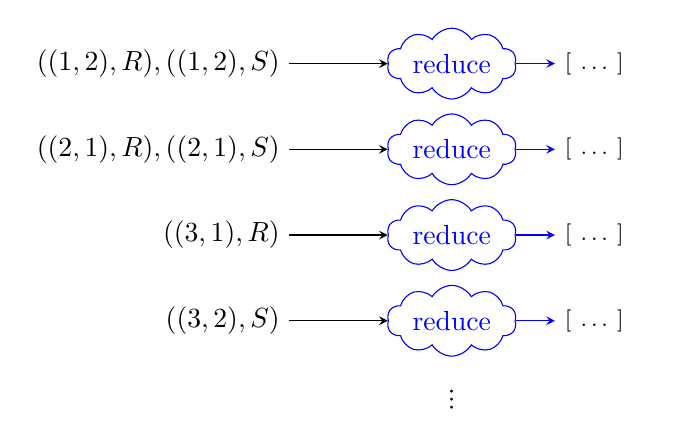
\begin{tikzpicture}
\node (reduce1) at (0,0) [blue,cloud, draw,cloud puffs=10,cloud puff arc=120, aspect=2.5, inner sep=2pt] {reduce};
\node (input1) [left=1.25cm of reduce1] {$((1,2), R), ((1,2), S)$};
\node (answer1) [right= 0.5cm of reduce1,text width=1cm] {\footnotesize $[\ \ldots\ ]$};
\draw[->,>=stealth] (input1) -- (reduce1);
\draw[blue,->,>=stealth] (reduce1) -- (answer1);

\node (reduce2) [below=5pt of reduce1] [blue,cloud, draw,cloud puffs=10,cloud puff arc=120, aspect=2.5, inner sep=2pt] {reduce};
\node (input2) [left=1.25cm of reduce2] {$((2,1), R), ((2,1), S)$};
\node (answer2) [right= 0.5cm of reduce2,text width=1cm] {\footnotesize $[\ \ldots\ ]$};
\draw[->,>=stealth] (input2) -- (reduce2);
\draw[blue,->,>=stealth] (reduce2) -- (answer2);

\node (reduce3) [below=5pt of reduce2] [blue,cloud, draw,cloud puffs=10,cloud puff arc=120, aspect=2.5, inner sep=2pt] {reduce};
\node (input3) [left=1.25cm of reduce3] {$((3,1), R)$};
\node (answer3) [right= 0.5cm of reduce3,text width=1cm] {\footnotesize $[\ \ldots\ ]$};
\draw[->,>=stealth] (input3) -- (reduce3);
\draw[blue,->,>=stealth] (reduce3) -- (answer3);

\node (reduce4) [below=5pt of reduce3] [blue,cloud, draw,cloud puffs=10,cloud puff arc=120, aspect=2.5, inner sep=2pt] {reduce};
\node (input4) [left=1.25cm of reduce4] {$((3,2), S)$};
\node (answer4) [right= 0.5cm of reduce4,text width=1cm] {\footnotesize $[\ \ldots\ ]$};
\draw[->,>=stealth] (input4) -- (reduce4);
\draw[blue,->,>=stealth] (reduce4) -- (answer4);

\node [below of=reduce4, rotate=90] {...};
\end{tikzpicture}}
\end{column}
\end{columns}

\begin{itemize}[-,noitemsep]
\item \alert{$R\cap S$}: reducer keeps keys with both values.
\item \alert{$R\cup S$}: reducer keeps all unique keys.
\item \alert{$R-S$}: reducer keeps keys with value $R$ but not $S$.
\end{itemize}
\end{frame}

%
% ----------------------------------------------------------------------------------------------------
%


\begin{frame}
\vskip2em

\begin{block}{Join \alert{$R \Join_{x=y} S$}}
\begin{itemize}[-,noitemsep,topsep=-10pt]
\item \lstinline!map()!: emit tuples from $R$ with attribute $R.x$ as key, and tuples from $S$ with $S.y$ as key.
\item \lstinline!reduce()!: iterate through the incoming lists with matching values!
\end{itemize}
\end{block}

Example: $R \Join_{b=c} S$

\begin{center}
\scalebox{0.75}{
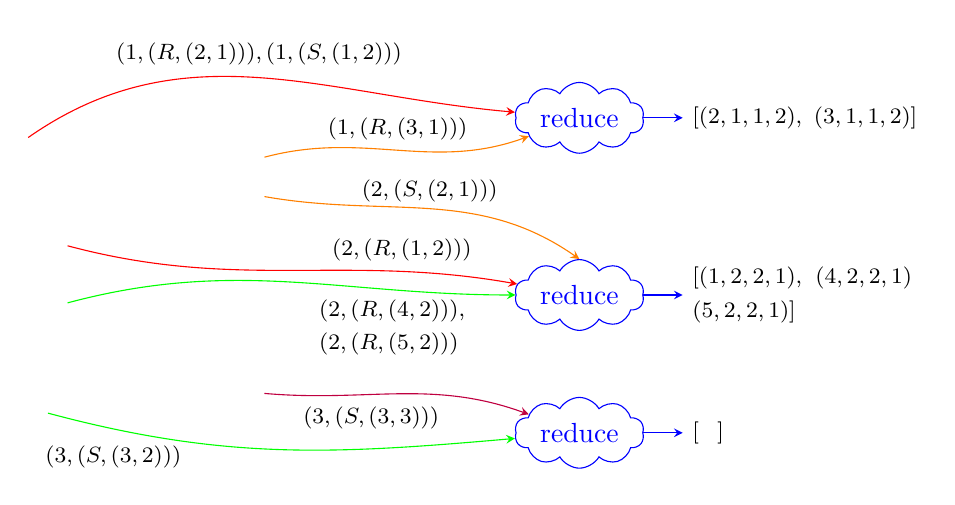
\begin{tikzpicture}
\MRclusterExample
\node (reduce1) at (8,3.75) [blue,cloud, draw,cloud puffs=10,cloud puff arc=120, aspect=2.5, inner sep=2pt] {reduce};
\draw [draw=red,->,>=stealth] (1,3.5) to[out=35,in=175] node[above,yshift=1pt]{\footnotesize $(1, (R, (2,1))), (1, (S, (1,2)))$} (reduce1);
\draw [draw=orange,->,>=stealth] (4,3.25) to[out=15,in=200] node[above]{\footnotesize $(1, (R, (3,1)))$} (reduce1);
\node (answer1) [right= 0.5cm of reduce1] {\footnotesize $[(2,1,1,2),\ (3,1,1,2)]$};
\draw[blue,->,>=stealth] (reduce1) -- (answer1);

\node (reduce2) at (8,1.5) [blue,cloud, draw,cloud puffs=10,cloud puff arc=120, aspect=2.5, inner sep=2pt] {reduce};
\draw [draw=red,->,>=stealth] (1.5,2.125) to[out=345,in=170] node[above,xshift=40pt]{\footnotesize $(2, (R, (1,2)))$} (reduce2);
\draw [draw=orange,->,>=stealth] (4,2.75) to[out=350,in=145] node[above,yshift=-1pt]{\footnotesize $(2, (S, (2,1)))$} (reduce2.north);
\draw [draw=green,->,>=stealth] (1.5,1.4) to[out=15,in=180] node[below,yshift=-3pt,xshift=25pt,text width=1cm]{\footnotesize $(2, (R, (4,2))),$ $(2, (R, (5,2)))$} (reduce2);
\node (answer2) [right= 0.5cm of reduce2,text width=1cm] {\footnotesize $[(1,2,2,1),\ (4,2,2,1)$ $(5,2,2,1)]$};
\draw[blue,->,>=stealth] (reduce2) -- (answer2);


\node (reduce3) at (8,-0.25) [blue,cloud, draw,cloud puffs=10,cloud puff arc=120, aspect=2.5, inner sep=2pt] {reduce};
\draw [draw=green,->,>=stealth] (1.25,0) to[out=345,in=185] node[below,xshift=-60pt,yshift=5pt]{\footnotesize $(3, (S, (3,2)))$} (reduce3);
\draw [draw=purple,->,>=stealth] (4,0.25) to[out=355,in=160] node[below,xshift=-10pt,yshift=-1pt]{\footnotesize $(3, (S, (3,3)))$} (reduce3);
\node (answer3) [right= 0.5cm of reduce3,text width=1cm] {\footnotesize $[\ \ ]$};
\draw[blue,->,>=stealth] (reduce3) -- (answer3);
\end{tikzpicture}}
\end{center}
\end{frame}

%
% ----------------------------------------------------------------------------------------------------
%


\begin{frame}{SQL in Map/Reduce}

Except for fixpoint-semantics recursion, pretty much all of SQL can be easily computed with Map/Reduce:
\begin{itemize}[-]

\item The ``bag'' versions of the set operations is also easily done in Map/Reduce: all that is needed is to count the number of (reduce) keys with value $R$ or $S$ in each stream.

\item Aggregations (\lstinline[style=SQL]!GROUP BY!) and set functions are also easily computable with Map/Reduce.

\item Duplicate elimination is also trivial when the reduce key is a tuple.
\end{itemize}
\end{frame}


\newsavebox{\mapreduceStepI}
\begin{lrbox}{\mapreduceStepI}
\begin{tikzpicture}
\MRclusterExample
%
\node (n4t2) [below=0em of n4t1] {\alert{\lstinline[style=cmput391]!-:t(2,1):-!}};
\node (n4t3) [below=0em of n4t2] {\alert{\lstinline[style=cmput391]!-:t(3,1):-!}};
%
\node (reduce) at (6.5,2) [blue,cloud, draw,cloud puffs=10,cloud puff arc=120, aspect=2.5, inner sep=2pt] {reduce};
\draw [draw=red,->,>=stealth] (1,3.5) to[out=45,in=135] node[above]{\footnotesize  $(k, (2,1))$} (reduce);
\draw [draw=red,->,>=stealth] (4,2.5) to node[above]{\footnotesize  $(k, (3,1))$} (reduce);
\draw[densely dotted,purple,->,>=stealth] (reduce) to[out=250, in=10] (4,0.5);
\end{tikzpicture}
\end{lrbox}

\newsavebox{\mapreduceStepII}
\begin{lrbox}{\mapreduceStepII}
\begin{tikzpicture}
\MRclusterExample
%
\node (n4t2) [below=0em of n4t1] {\alert{\lstinline[style=cmput391]!-:t(2,1):-!}};
\node (n4t3) [below=0em of n4t2] {\alert{\lstinline[style=cmput391]!-:t(3,1):-!}};
%
\node (reduce) at (6.5,2) [blue,cloud, draw,cloud puffs=10,cloud puff arc=120, aspect=2.5, inner sep=2pt] {reduce};
\draw [draw=red,->,>=stealth] (4,1) node[below right]{\footnotesize $(k, [(2),(3)])$} -- (reduce);
\node (answer) [below right= 1cm and 0.125cm of reduce] {\footnotesize $[(2),(3)]$};
\draw[blue,->,>=stealth] (reduce) -- (answer);
\end{tikzpicture}
\end{lrbox}



%
% ----------------------------------------------------------------------------------------------------
%


\begin{frame}{Multi-operator Queries}

We answer a query like $\pi_{a_1,\ldots,a_n}(\sigma_C(R))$ in two map/reduce processes:
\begin{enumerate}[(1),noitemsep]
\item Materialize $\text{\lstinline!t!} \leftarrow\sigma_C(R)$ in a temporary table.
\item Compute $\pi_{a_1,\ldots,a_n}(\text{\lstinline!t!})$ over the temporary table.
\end{enumerate}

\begin{center}
\scalebox{0.6}{
\begin{tikzpicture}
\node at (0,5.25) [blue] {step 1};
\node at (0,0) [anchor=south] {\usebox{\mapreduceStepI}};
\node at (9.5,5.25) [blue] {step 2};
\node at (9.5,0) [anchor=south] {\usebox{\mapreduceStepII}};
\end{tikzpicture}}
\end{center}

\end{frame}


%
% ----------------------------------------------------------------------------------------------------
%


\begin{frame}{How many reducers to use?}

Recall that in every map/reduce computation:
\begin{itemize}[-,noitemsep]
\item The number of \lstinline!map()! tasks is the same as the number of computing nodes.
\item The number of \lstinline!reduce()! tasks is the same \textbf{as the number} of reduce keys!
\end{itemize}

\vskip1em

\begin{block}{Why does this matter?}
If the first step uses a single reducer:
\begin{itemize}[-,noitemsep]
 \item A single node will store all tuples from the first step\footnotemark.
 \item Only one \lstinline!map()! task will run in the second step.
\end{itemize}
\end{block}
\footnotetext{Of course, the cluster may be setup to replicate the data across multiple nodes, alleviating the problem.}
\end{frame}


%
% ----------------------------------------------------------------------------------------------------
%


\begin{frame}

\vskip2em

\begin{block}{Selection \alert{$\sigma_C R$} with \textbf{multiple} reducers.}
\begin{itemize}[-,noitemsep,topsep=-10pt]
\item \lstinline!map()!: go through every tuple in the node, emit each tuple satisfying the selection using the tuple itself\footnotemark as key.
\item \lstinline!reduce()!: collect all copies of each tuple.
\end{itemize}
\end{block}

Example: $\sigma_{b=1} R$

\begin{center}
\scalebox{0.75}{
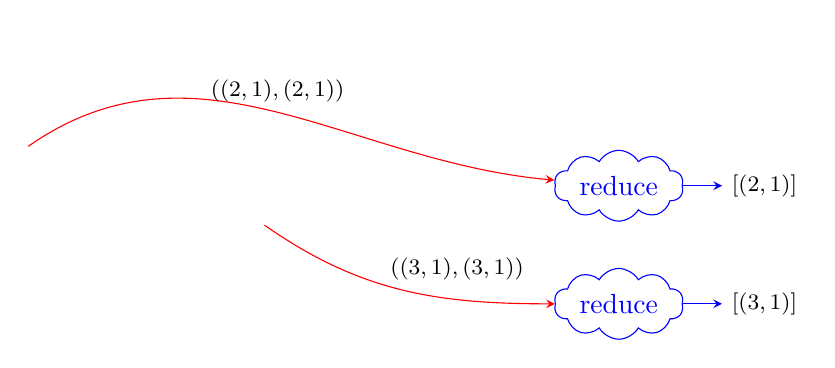
\begin{tikzpicture}
\MRclusterExample
\node (reduceA) at (8.5,3) [blue,cloud, draw,cloud puffs=10,cloud puff arc=120, aspect=2.5, inner sep=2pt] {reduce};
\node (reduceB) at (8.5,1.5) [blue,cloud, draw,cloud puffs=10,cloud puff arc=120, aspect=2.5, inner sep=2pt] {reduce};
\draw [draw=red,->,>=stealth] (1,3.5) to[out=35,in=175] node[above]{\footnotesize  $((2,1), (2,1))$} (reduceA);
\draw [draw=red,->,>=stealth] (4,2.5) to[out=325,in=180] node[above,xshift=20pt]{\footnotesize  $((3,1), (3,1))$} (reduceB);
\node (answerA) [right= 0.5cm of reduceA] {\footnotesize $[(2,1)]$};
\node (answerB) [right= 0.5cm of reduceB] {\footnotesize $[(3,1)]$};
\draw[blue,->,>=stealth] (reduceA) -- (answerA);
\draw[blue,->,>=stealth] (reduceB) -- (answerB);
\end{tikzpicture}}
\end{center}

\vskip1em 

\footnotetext{A hash of the tuple would also work, and save on communication costs.}

\end{frame}


%
% ----------------------------------------------------------------------------------------------------
%


\begin{frame}
How many reducers should one use?
\begin{itemize}[-]
\item A single reducer can intuitively act as the ``server-side'' transaction process for each request by a connected user/application.
\item With multiple reducers (which run as independent processes), one can spread the tuples in the ``temporary table'' across more nodes, increasing the number of \lstinline!map()! tasks that \textbf{run in parallel} in subsequent steps.
\item Thus, multiple reducers seem better for intermediate query operations, while the single reducer approach seems better for the root node of the query.
\end{itemize}
\end{frame}


%
% ----------------------------------------------------------------------------------------------------
%


\begin{frame}[fragile]{Map/Reduce in NoSQL systems}

Some document stores like CouchDB use Map/Reduce for parallel query processing~\footnote{\url{https://docs.couchdb.org/en/stable/ddocs/views/intro.html}}. 

For example, one can use \lstinline!map()! functions to select multiple (fragments) of JSON documents in the cluster that satisfy a predicate, querying all documents in the cluster simultaneously, and the \lstinline!reduce()! function to compute an aggregate answer.

\begin{columns}[onlytextwidth]
\begin{column}{0.5\textwidth}
\begin{lstlisting}[basicstyle=\ttfamily\scriptsize]
function map(doc) {
  if(doc.author.includes("Manning")) {
      emit(doc.publisher,
       doc.title);
  }
}
\end{lstlisting}
\end{column}
\quad\begin{column}{0.45\textwidth}
\begin{lstlisting}[basicstyle=\ttfamily\scriptsize]
function reduce(key, values) {
  var cnt = 0;
    for(var idx in values) {
      cnt = cnt + 1;
  }
  return (key, cnt);
}\end{lstlisting}
\end{column}
\end{columns}
\end{frame}



\section{Parting Thoughts}

\begin{frame}

High Performance Computing architectures, in particular, shared-nothing clusters of computers organized into a ``cloud'', are becoming the norm in supporting database applications.

Two key advantages of this approach are distributing the data across nodes to reduce the risk of data loss and increase availability of the data.

The compromise is that updates to the data require a lot more effort: multiple nodes need to coordinate via the network, which is much slower.

As a result, most NoSQL systems do not support complex constraints and do not offer full SQL support.
\end{frame}
\end{document}